\documentclass[12pt,a4paper]{article}
\usepackage[fontsize=13pt]{scrextend}
\usepackage[left=3cm,right=1.5cm,top=2cm,bottom=2cm,headheight=14pt,headsep=0.35cm,footskip=0.9cm]{geometry}
\usepackage{fontspec}
\setmainfont{Tinos}
\usepackage{graphicx}
\usepackage{float}
\usepackage{xcolor}
\usepackage{array,tabularx,longtable}
\usepackage{booktabs}
\newcolumntype{L}[1]{>{\raggedright\arraybackslash}p{#1}}
\usepackage{chngcntr}
\counterwithin{figure}{section}
\counterwithin{table}{section}
\renewcommand{\figurename}{Hình}
\renewcommand{\tablename}{Bảng}
\usepackage{fancyhdr}
\usepackage{setspace}
\usepackage{enumitem}
\usepackage{ragged2e}
\usepackage{calc}
\usepackage{hyperref}
\hypersetup{colorlinks=false,pdfborder={0 0 0}}

\definecolor{headingblue}{RGB}{0,0,0}
\definecolor{placeholdergray}{RGB}{0,0,0}
\setstretch{1.5}
\setlength{\parindent}{0pt}
\setlength{\parskip}{3pt}
\setlist{nosep,leftmargin=*}

\pagestyle{fancy}
\fancyhf{}
\fancyhead[R]{\scriptsize\color{placeholdergray}Tiểu luận tốt nghiệp}
\fancyfoot[C]{\small\thepage}
\renewcommand{\headrulewidth}{0pt}
\renewcommand{\footrulewidth}{0pt}

\newcommand{\ph}[1]{{\itshape\color{placeholdergray}[#1]}}
\newcommand{\chap}[1]{\stepcounter{section}\phantomsection\addcontentsline{toc}{section}{#1}\vspace*{0.1cm}{\bfseries\color{headingblue}\large #1}\par\vspace{6pt}}
\newcommand{\secA}[1]{\phantomsection\addcontentsline{toc}{subsection}{#1}\vspace{5pt}{\bfseries\color{headingblue}#1}\par\vspace{2pt}}
\newcommand{\secB}[1]{\phantomsection\addcontentsline{toc}{subsubsection}{#1}\vspace{4pt}{\bfseries\color{headingblue}\small #1}\par\vspace{1pt}}

\makeatletter
\renewcommand\tableofcontents{%
    \begin{center}{\bfseries\Large MỤC LỤC}\end{center}%
    \vspace{0.45cm}%
    \@starttoc{toc}%
}
\makeatother

\begin{document}

% Trang bìa
\thispagestyle{empty}
\begin{center}
\vspace*{0.45cm}
{\bfseries\Large BỘ GIÁO DỤC VÀ ĐÀO TẠO\\[4pt]}
{\bfseries\Large TRƯỜNG ĐẠI HỌC TÂN TẠO\\[4pt]}
{\bfseries\Large KHOA CÔNG NGHỆ THÔNG TIN\\[1.0cm]}

\includegraphics[width=4.0cm]{image/Mau_Luan_Van_Tot_Nghiep_html_cf243cb600b36d28.png}\\[1.0cm]
{\bfseries\LARGE TIỂU LUẬN TỐT NGHIỆP ĐẠI HỌC\\[1.0cm]}
{\bfseries\LARGE XÂY DỰNG HỆ THỐNG PHÁT HIỆN TIN GIẢ TIẾNG VIỆT\\[10pt]}
{\itshape\Large (Hệ thống ShieldAI)}
\end{center}

\vspace{1.8cm}
\begin{center}
\begin{tabular}{ll}
\textbf{Ngành:} & Khoa Học Máy Tính\\[8pt]
\textbf{Mã số:} & 7480101\\[8pt]
\textbf{Khóa:} & 2022\\[20pt]
\textbf{Sinh viên thực hiện:} & Hà Minh Chiến\\[8pt]
\textbf{Mã số sinh viên:} & 2202095\\[8pt]
\textbf{Giảng viên hướng dẫn:} & Thầy Trần Ngọc Anh\\
\end{tabular}
\end{center}
\vfill
\begin{center}{\bfseries\Large TÂY NINH, THÁNG 06 NĂM 2026}\end{center}
\newpage
\setcounter{page}{2}

% Trang phê duyệt
\begin{center}\vspace*{2.2cm}{\bfseries\Large TRANG PHÊ DUYỆT}\end{center}
\vspace{0.7cm}
Tiểu luận đã được trình và bảo vệ trước Hội đồng chấm tiểu luận tốt nghiệp.

\vspace{0.4cm}
Ngày bảo vệ: 26/06/2026\\
Kết quả: 9.5/10 điểm (Tốt)

\vspace{1.2cm}
\begin{tabularx}{\textwidth}{>{\centering\arraybackslash}X>{\centering\arraybackslash}X}
\textbf{GIẢNG VIÊN HƯỚNG DẪN} & \textbf{GIẢNG VIÊN PHẢN BIỆN}\\
(Ký và ghi rõ họ tên) & (Ký và ghi rõ họ tên)\\[3.9cm]
\end{tabularx}
\vspace{0.6cm}
\begin{center}
\textbf{CHỦ TỊCH HỘI ĐỒNG}\\
(Ký và ghi rõ họ tên)
\end{center}
\newpage

\begin{center}\vspace*{2.4cm}{\bfseries\Large LỜI CẢM ƠN}\end{center}
\vspace{0.5cm}
Trong suốt thời gian thực hiện tiểu luận tốt nghiệp với đề tài \textbf{"Xây dựng hệ thống phát hiện tin giả tiếng Việt"}, em đã nhận được rất nhiều sự quan tâm, giúp đỡ và động viên từ Quý thầy cô, gia đình và bạn bè.

Trước tiên, em xin bày tỏ lòng biết ơn sâu sắc đến Thầy \textbf{Trần Ngọc Anh}, người đã tận tình hướng dẫn, định hướng khoa học và truyền đạt những kiến thức quý báu cho em trong suốt quá trình triển khai và hoàn thiện tiểu luận. Sự chỉ bảo tận tâm của Thầy không chỉ giúp em giải quyết các vấn đề kỹ thuật phức tạp mà còn rèn luyện cho em tư duy nghiên cứu độc lập.

Em cũng xin gửi lời cảm ơn chân thành đến Ban Giám hiệu, Quý thầy cô Khoa \textbf{Công nghệ Thông tin} trường \textbf{Đại học Tân Tạo (TTU)} đã tạo điều kiện học tập tốt nhất, cũng như trang bị cho em nền tảng kiến thức vững chắc trong suốt những năm tháng giảng đường.

Bên cạnh đó, em xin cảm ơn những người bạn đồng trang lứa đã cùng nhau chia sẻ tài liệu, thảo luận và đóng góp nhiều ý kiến hữu ích giúp em hoàn thiện hệ thống ShieldAI.

Cuối cùng, em xin gửi lời tri ân sâu sắc nhất đến gia đình, những người luôn là chỗ dựa tinh thần vững chắc, động viên và tạo mọi điều kiện thuận lợi nhất để em có thể tập trung học tập và hoàn thành chương trình đại học.

Mặc dù đã có nhiều cố gắng trong quá trình thực hiện, nhưng do hạn chế về mặt thời gian và kinh nghiệm thực tiễn, tiểu luận khó tránh khỏi những thiếu sót. Em rất mong nhận được sự góp ý và chỉ bảo thêm từ Quý thầy cô và Hội đồng bảo vệ để hệ thống được hoàn thiện hơn.

Một lần nữa, em xin chân thành cảm ơn!
\newpage

\begin{center}\vspace*{2.4cm}{\bfseries\Large TÓM TẮT TIỂU LUẬN}\end{center}
\vspace{0.5cm}
Sự bùng nổ của mạng xã hội và truyền thông số tại Việt Nam đã mang lại nhiều lợi ích to lớn, nhưng đồng thời cũng kéo theo hệ lụy nghiêm trọng từ việc lan truyền tin giả (Fake News). Tin giả không chỉ gây hoang mang dư luận mà còn ảnh hưởng tiêu cực đến an ninh, chính trị và nền kinh tế. Nhằm giải quyết vấn đề cấp thiết này, tiểu luận trình bày quá trình nghiên cứu và phát triển hệ thống ShieldAI – một ứng dụng Web tự động có khả năng tự động phát hiện và phân loại độ tin cậy của văn bản tiếng Việt.

Chính của hệ thống là mô hình học sâu \textbf{PhoBERT} được tinh chỉnh đầy đủ theo kiến trúc Phân loại Chuỗi (Fine-tuned Sequence Classification) trên tập dữ liệu tiếng Việt đa dạng. Một đặc điểm của hệ thống là tích hợp cơ chế giải thích dựa trên đặc trưng kinh nghiệm (Heuristics-based Explanation). Cơ chế này giúp khắc phục nhược điểm "hộp đen" của các mô hình học sâu bằng cách không chỉ cung cấp kết quả phân loại mà còn diễn giải nguyên nhân thông qua việc phân tích từ khóa, mật độ viết hoa, cảm xúc (sentiment) và tính chủ quan của văn bản.

Kết quả thực nghiệm cho thấy mô hình đạt độ chính xác (Accuracy) \textbf{96.32\%} và F1-Score \textbf{93.42\%}. Các chỉ số này được đánh giá nghiêm ngặt trên tập kiểm thử nội bộ (Test Set) chiếm 12\% (khoảng 2.716 mẫu). Tập dữ liệu được lấy mẫu phân tầng (Stratified Split) từ kho ngữ liệu tổng hợp hơn 22.000 bài báo đã qua bước làm sạch trùng lặp (Deduplication) để giảm thiểu hiện tượng rò rỉ dữ liệu (Data Leakage). Mặc dù cần thêm các phép thử ngoại lai (External Test) trong tương lai để kiểm chứng tính khái quát hóa, mức hiệu năng hiện tại đã cho thấy độ ổn định cao của kiến trúc đề xuất. Hơn thế nữa, hệ thống được triển khai với kiến trúc Client-Server, tích hợp giao diện dễ sử dụng, trực tiếp hỗ trợ người dùng trong việc xây dựng không gian thông tin số an toàn tại Việt Nam.

\vspace{0.65cm}
\textbf{Từ khóa:} Phát hiện tin giả, PhoBERT, Heuristics, Sequence Classification, NLP
\newpage

\begin{center}\vspace*{2.5cm}{\bfseries\Large ABSTRACT}\end{center}
\vspace{0.5cm}
The explosive growth of social media and digital communication in Vietnam has brought significant benefits but has also led to severe consequences due to the proliferation of Fake News. Fake news not only causes public confusion but also negatively impacts security, politics, and the economy. To address this urgent issue, this thesis presents the research and development process of ShieldAI – an intelligent Web application capable of automatically detecting and classifying the reliability of Vietnamese texts.

The core of the system is the \textbf{PhoBERT} deep learning model, which is fine-tuned end-to-end for Sequence Classification on a diverse Vietnamese dataset. A distinctive feature of ShieldAI is the integration of a Heuristics-based Explanation mechanism. This mechanism helps overcome the "black-box" limitations of traditional deep learning models by not only providing classification results but also explaining the reasoning through the analysis of keywords, capitalization density, sentiment, and text subjectivity.

Experimental results demonstrate that the model achieves an Accuracy of \textbf{96.32\%} and an F1-Score of \textbf{93.42\%}. These metrics were rigorously evaluated on a 12\% hold-out Test Set (2,716 samples), which was generated via Stratified Split from a combined dataset of over 22,000 articles perfectly deduplicated to prevent data leakage. Although future external out-of-distribution testing is required to fully eliminate the risk of source memorization, the current performance establishes a solid baseline for the proposed architecture. Furthermore, the application is deployed with a Client-Server architecture and a user-friendly interface, providing practical support for building a safe digital space in Vietnam.

\vspace{0.65cm}
\textbf{Keywords:} Fake News Detection, PhoBERT, Heuristics, Sequence Classification, NLP
\newpage

\tableofcontents
\newpage

\renewcommand{\listfigurename}{\begin{center}{\bfseries\Large DANH MỤC HÌNH ẢNH}\end{center}}
\listoffigures
\newpage

\renewcommand{\listtablename}{\begin{center}{\bfseries\Large DANH MỤC BẢNG BIỂU}\end{center}}
\listoftables
\newpage

\begin{center}{\bfseries\Large DANH MỤC TỪ VIẾT TẮT}\end{center}
\vspace{0.35cm}
\begingroup
\renewcommand{\theHtable}{frontabbr}
\begin{longtable}{L{0.20\textwidth}L{0.70\textwidth}}
\toprule
\textbf{Từ viết tắt} & \textbf{Giải thích}\\
\midrule
\endfirsthead
\toprule
\textbf{Từ viết tắt} & \textbf{Giải thích}\\
\midrule
\endhead
AI & Trí tuệ nhân tạo (Artificial Intelligence).\\
API & Giao diện lập trình ứng dụng (Application Programming Interface).\\
BERT & Mô hình biểu diễn ngôn ngữ hai chiều từ Transformer (Bidirectional Encoder Representations from Transformers).\\
CPU & Bộ vi xử lý trung tâm (Central Processing Unit).\\
DDoS & Tấn công từ chối dịch vụ phân tán (Distributed Denial of Service).\\
DL & Học sâu (Deep Learning).\\
DOM & Mô hình Đối tượng Tài liệu (Document Object Model).\\
EDA & Khai phá và Phân tích Dữ liệu (Exploratory Data Analysis).\\
ERD & Sơ đồ Thực thể - Mối quan hệ (Entity-Relationship Diagram).\\
GPU & Bộ xử lý đồ họa (Graphics Processing Unit).\\
HTML & Ngôn ngữ đánh dấu siêu văn bản (HyperText Markup Language).\\
JSON & Định dạng trao đổi dữ liệu (JavaScript Object Notation).\\
JWT & Mã thông báo Web JSON (JSON Web Token).\\
LSTM & Bộ nhớ ngắn hạn dài (Long Short-Term Memory).\\
ML & Học máy (Machine Learning).\\
MLOps & Vận hành Học máy (Machine Learning Operations).\\
NLP & Xử lý Ngôn ngữ Tự nhiên (Natural Language Processing).\\
ORM & Ánh xạ đối tượng - quan hệ (Object-Relational Mapping).\\
RAM & Bộ nhớ truy cập ngẫu nhiên (Random Access Memory).\\
RNN & Mạng nơ-ron hồi quy (Recurrent Neural Network).\\
SeqCls & Phân loại chuỗi (Sequence Classification).\\
SVM & Máy học véc-tơ hỗ trợ (Support Vector Machine).\\
TF-IDF & Tần suất xuất hiện của từ - Nghịch đảo tần suất văn bản (Term Frequency-Inverse Document Frequency).\\
UI/UX & Giao diện/Trải nghiệm người dùng (User Interface / User Experience).\\
URL & Định vị tài nguyên thống nhất (Uniform Resource Locator).\\
VRAM & Bộ nhớ truy cập ngẫu nhiên đồ họa (Video Random Access Memory).\\
XAI & Trí tuệ nhân tạo minh bạch (Explainable Artificial Intelligence).\\
\bottomrule
\end{longtable}
\endgroup
\newpage

\chap{CHƯƠNG 1: GIỚI THIỆU}
\secA{1.1. Đặt vấn đề}
Sự bùng nổ của mạng xã hội đã tạo điều kiện cho "tin giả" (Fake News) lan truyền, thao túng dư luận và gây rủi ro xã hội. Dù các mô hình Học sâu như Transformer và PhoBERT đã đạt nhiều tiến bộ trong việc phân tích văn bản, chúng vẫn bộc lộ hạn chế lớn là tính chất "hộp đen" và thiếu khả năng diễn giải kết quả cho người dùng cuối. Do đó, đề tài \textbf{"Xây dựng hệ thống phát hiện tin giả tiếng Việt (Hệ thống ShieldAI)"} được thực hiện nhằm giải quyết vấn đề này.

Đề tài tập trung nghiên cứu và xây dựng hệ thống phân loại tin giả dựa trên mô hình ngôn ngữ tiền huấn luyện PhoBERT kết hợp với mô hình phân loại chuỗi (Sequence Classification). Hệ thống này tập trung khai thác các đặc trưng ngữ nghĩa từ văn bản để đưa ra phán quyết chuẩn xác. Đặc biệt, nhằm tăng khả năng giải thích quyết định của hệ thống và cải thiện khả năng giải thích của mô hình, nghiên cứu đề xuất tích hợp một Động cơ giải thích (Explanation Engine) độc lập dựa trên luật và các đặc trưng kinh nghiệm (Heuristics) --- nhằm bóc tách các dấu hiệu thao túng cảm xúc, văn phong giật gân, sự lạm dụng dấu câu --- từ đó góp phần nâng cao khả năng giải thích cho quyết định phân loại của mô hình.

Để đánh giá tính khả thi của phương pháp đề xuất, mô hình được triển khai và kiểm thử trên bộ dữ liệu tin tức tiếng Việt đã được gán nhãn. Các chỉ số đánh giá chính như Accuracy, Precision, Recall và F1-Score được sử dụng để phân tích hiệu năng của mạng phân loại. Kết quả thực nghiệm, tính hiệu quả của cơ chế giải thích cùng các phân tích chi tiết sẽ được trình bày trong chương đánh giá của tiểu luận.

\secA{1.2. Mục tiêu nghiên cứu}
\secB{1.2.1. Mục tiêu tổng quát}
Phát triển nền tảng Web kiểm duyệt tin giả tiếng Việt tự động, ứng dụng kiến trúc AI tinh gọn (PhoBERT Fine-tuned Sequence Classification) và cơ chế giải thích dựa trên đặc trưng để minh bạch hóa quyết định, đồng thời quản lý lịch sử tra cứu của người dùng an toàn.

\secB{1.2.2. Mục tiêu cụ thể}
\begin{itemize}[label={--},leftmargin=0.75cm,itemsep=3pt]
\item \textbf{Hệ thống hóa lý thuyết:} Khảo cứu cơ sở lý thuyết về Xử lý Ngôn ngữ Tự nhiên (NLP), mô hình PhoBERT và các phương pháp giải thích mô hình (XAI).
\item \textbf{Tinh chỉnh mô hình PhoBERT:} Áp dụng kỹ thuật Fine-tuning trên kiến trúc PhoBERT để thực hiện tác vụ phân loại chuỗi (Sequence Classification) cho bài toán phát hiện tin giả.
\item \textbf{Xây dựng cơ chế giải thích:} Đề xuất và cài đặt module giải thích dựa trên luật (Rule-based Heuristics) nhằm cung cấp lý do phân loại một cách minh bạch.
\item \textbf{Phát triển hệ thống nguyên mẫu:} Triển khai kiến trúc Client-Server để tích hợp mô hình AI thành một ứng dụng thực tiễn, hỗ trợ người dùng kiểm chứng thông tin.
\item \textbf{Đánh giá hiệu năng:} Thực nghiệm và so sánh độ chính xác của kiến trúc đề xuất với các thuật toán Học máy truyền thống.
\end{itemize}

\secA{1.3. Đối tượng và phạm vi nghiên cứu}
\secB{1.3.1. Đối tượng nghiên cứu}
Bao gồm: (1) Mô hình ngôn ngữ tiền huấn luyện PhoBERT được tinh chỉnh; (2) Pipeline tiền xử lý \texttt{preprocess\_text}; (3) Giải thích rule-based (\texttt{ExplanationEngine}); và (4) Công nghệ Web (FastAPI, Next.js, SQLite).

\secB{1.3.2. Phạm vi nghiên cứu}
\begin{itemize}[label={--},leftmargin=0.75cm,itemsep=3pt]
\item \textbf{Mục tiêu phân loại:} Thay vì tiếp cận theo hướng nhị phân cứng nhắc, hệ thống ShieldAI cung cấp trải nghiệm người dùng (UX) tinh tế hơn với 3 mức độ cảnh báo: Tin thật (Xác suất < 35\%), Đáng ngờ (35\% - 74\%), và Tin giả (Xác suất $\ge$ 75\%).
\item \textbf{Thuật toán:} Tập trung vào kiến trúc PhoBERT Fine-tuned Sequence Classification, lấy vector [CLS] 768 chiều từ PhoBERT đưa qua mạng nơ-ron truyền thẳng đa tầng.
\item \textbf{Cấu trúc Triển khai ứng dụng (Deployment):} Tiểu luận được hệ thống hóa theo kiến trúc Client-Server đầy đủ chức năng. Giao diện người dùng (Frontend) được phát triển bằng Next.js 14 hỗ trợ tương tác ổn định; Máy chủ (Backend) sử dụng FastAPI bất đồng bộ cho hiệu năng cao; Dữ liệu lịch sử quét tin giả được lưu trữ an toàn bằng SQLite. Đặc biệt, hệ thống tích hợp Trình thu thập dữ liệu (Web Crawler) bằng BeautifulSoup giúp tự động cào nội dung bài báo trực tiếp từ URL, cải thiện đáng kể trải nghiệm người dùng (UX) thay vì ép người dùng dán văn bản thuần túy.
\end{itemize}

\secA{1.4. Phương pháp nghiên cứu}
Để giải quyết đầy đủ bài toán phát hiện tin giả và xây dựng một ứng dụng tích hợp, tiểu luận áp dụng kết hợp các phương pháp nghiên cứu sau:
\begin{itemize}[label={--},leftmargin=0.75cm,itemsep=3pt]
\item \textbf{Phương pháp nghiên cứu tài liệu (Literature Review):} Khảo sát, tổng hợp và phân tích các bài báo khoa học, tài liệu chuyên ngành về Xử lý ngôn ngữ tự nhiên (NLP), kiến trúc Transformer (đặc biệt là họ mô hình PhoBERT), và các thuật toán phân loại Học máy. Phương pháp này giúp xây dựng cơ sở lý thuyết cho tiểu luận.
\item \textbf{Phương pháp thu thập và tiền xử lý dữ liệu (Data Preprocessing):} Xây dựng các kịch bản thu thập dữ liệu (Web Crawler) tự động hóa và áp dụng kỹ thuật làm sạch văn bản, chuẩn hóa ngôn ngữ tiếng Việt (sử dụng thư viện PyVi) để tạo ra tập ngữ liệu đầu vào chất lượng, khử nhiễu trước khi đưa vào huấn luyện mô hình.
\item \textbf{Phương pháp thực nghiệm và mô hình hóa (Experimental \& Modeling):} Thiết kế, tinh chỉnh (Fine-tuning) kiến trúc mô hình ngôn ngữ tiền huấn luyện PhoBERT cho bài toán Phân loại Chuỗi. Đồng thời, nghiên cứu và lập trình Cơ chế giải thích dựa trên đặc trưng hình thức (Heuristic Explanation Engine) để minh bạch hóa quá trình ra quyết định của trí tuệ nhân tạo.
\item \textbf{Phương pháp thống kê và đánh giá (Statistical Evaluation):} Sử dụng phương pháp đánh giá trên tập kiểm thử độc lập (Hold-out Test Set) và các độ đo tiêu chuẩn trong Học máy (Precision, Recall, F1-Score, Ma trận nhầm lẫn - Confusion Matrix) để đánh giá định lượng hiệu năng mô hình một cách khách quan.
\item \textbf{Phương pháp kỹ nghệ phần mềm (Software Engineering):} Áp dụng quy trình phát triển được triển khai để thiết kế kiến trúc phân tán 3 tầng (Client-Server), lập trình giao diện người dùng (Next.js) và tích hợp API máy chủ (FastAPI), qua đó hiện thực hóa mô hình AI thành một phần mềm thực tiễn.
\end{itemize}

\secA{1.5. Ý nghĩa khoa học và thực tiễn}
\textbf{Về mặt khoa học (Tính mới của đề tài):} Thay vì tập trung phát triển một thuật toán học sâu mới độc lập (tiềm ẩn rủi ro về độ ổn định), đóng góp chính của tiểu luận nằm ở \textbf{Đổi mới Kiến trúc Tích hợp (Architectural Innovation)}. Cụ thể, tiểu luận đề xuất và thiết kế thành công một \textbf{"Kiến trúc Phân tách Ngữ nghĩa - Kinh nghiệm" (Decoupled Semantic-Heuristic Architecture)}. Trong kiến trúc này, việc phân loại ngữ nghĩa sâu được đảm nhiệm chính bởi PhoBERT, trong khi việc trích xuất lý do minh bạch được cô lập thành một Động cơ Giải thích bằng luật (Rule-based Explanation) chạy song song. Sự phân tách (Decoupling) này giải quyết một vấn đề thường gặp trong thực tiễn: Nó mang lại khả năng giải thích (XAI) cho mô hình học sâu mà không làm tăng độ trễ suy luận (Inference Latency) — một hạn chế về chi phí tính toán của các thuật toán XAI nội tại (như SHAP hay LIME) khi triển khai trên hệ thống Web thời gian thực.

\textbf{Về mặt thực tiễn:} Đề tài đã tích hợp các thành phần nghiên cứu kể trên thành hệ thống nguyên mẫu (prototype) ShieldAI. Đây là một công cụ hỗ trợ kiểm chứng thông tin, cung cấp cho cộng đồng mạng Việt Nam khả năng nhận diện tin giả kịp thời kèm theo những lời giải thích dễ hiểu. Bên cạnh đó, với kiến trúc API linh hoạt, hệ thống có khả năng mở rộng và tích hợp vào các mạng xã hội hoặc các công cụ kiểm duyệt nội dung tự động của các cơ quan báo chí trong tương lai.

\secA{1.6. Bố cục tiểu luận}
Ngoài phần Lời mở đầu và Kết luận, nội dung chính của tiểu luận được tổ chức thành 5 chương chính như sau:
\begin{itemize}[label={--},leftmargin=0.75cm,itemsep=3pt]
\item \textbf{Chương 1 - Mở đầu:} Trình bày bối cảnh, lý do chọn đề tài, mục tiêu, phạm vi nghiên cứu, các phương pháp tiếp cận và ý nghĩa tổng thể của dự án.
\item \textbf{Chương 2 - Cơ sở lý thuyết và tổng quan nghiên cứu:} Cung cấp các khái niệm nền tảng về bài toán tin giả, xử lý ngôn ngữ tự nhiên, kiến trúc mô hình PhoBERT, thuật toán Phân loại Chuỗi (Sequence Classification) và các độ đo đánh giá mô hình.
\item \textbf{Chương 3 - Phân tích thiết kế hệ thống:} Đi sâu vào kiến trúc phần mềm, mô hình dữ liệu (ERD), và chi tiết luồng dữ liệu (Data Pipeline) từ giai đoạn thu thập văn bản đến động cơ Giải thích Heuristic.
\item \textbf{Chương 4 - Kết quả thực nghiệm:} Trình bày các số liệu huấn luyện mô hình, kết quả kiểm thử hệ thống tự động (Unit Test) và minh họa giao diện sử dụng thực tế của phần mềm ShieldAI.
\item \textbf{Chương 5 - Tổng kết và hướng phát triển:} Đúc kết lại những thành tựu đã đạt được, chỉ ra các hạn chế còn tồn đọng và đề xuất các hướng nâng cấp hệ thống trong tương lai.
\end{itemize}
\newpage

\chap{CHƯƠNG 2: CƠ SỞ LÝ THUYẾT VÀ TỔNG QUAN NGHIÊN CỨU}
\secA{2.1. Các khái niệm nền tảng}
Để xây dựng một kiến trúc hệ thống phân tích tin giả phức tạp, việc nắm bắt các khái niệm chính mang tính chất nền tảng là điều kiện tiên quyết. Mục này sẽ trình bày và định nghĩa một cách khoa học các thuật ngữ chuyên ngành được sử dụng xuyên suốt trong tiểu luận.

\secB{2.1.1. Tin giả (Fake News) [3, 4] và Thông tin sai lệch}
Trong kỷ nguyên số, \textbf{Tin giả (Fake News) [3, 4]} được định nghĩa là những thông tin sai sự thật, bị bóp méo, hoặc bịa đặt, được trình bày dưới hình thức tin báo chí nhằm mục đích lừa dối người đọc. Điểm khác biệt mấu chốt của tin giả so với các lỗi sai sót báo chí thông thường nằm ở \textbf{động cơ (intent)}. Tin giả được tạo ra một cách có chủ đích nhằm thu lợi ích tài chính (thông qua việc thu hút lượt nhấp chuột - clickbait để lấy doanh thu quảng cáo) hoặc phục vụ các mục đích chính trị, thao túng tâm lý và định hướng dư luận xã hội.

Hội đồng Châu Âu (Council of Europe) phân loại thông tin sai lệch thành ba nhóm chính: \textit{Mis-information} (Thông tin sai nhưng không có ác ý), \textit{Dis-information} (Thông tin sai và có ác ý, bịa đặt), và \textit{Mal-information} (Thông tin có thật nhưng được dùng để bôi nhọ, hãm hại người khác). Tiểu luận này tập trung chủ yếu vào việc tự động nhận diện và phát hiện nhóm Dis-information, đặc biệt là các bài viết sử dụng ngôn từ kích động và cấu trúc câu lừa đảo trên mạng xã hội tiếng Việt.

Trong thực tiễn kiểm chứng thông tin (Fact-checking), việc xác định một văn bản có phải tin giả hay không hiếm khi chỉ dựa vào một yếu tố đơn lẻ, mà đòi hỏi sự đánh giá đa chiều qua nhiều khía cạnh trọng yếu. Dưới đây là các tiêu chí chính thường được sử dụng để phân loại và nhận diện tin giả:
\begin{itemize}[label={--},leftmargin=0.75cm,itemsep=3pt]
\item \textbf{Nguồn đăng tin và tính xác thực (Source Authenticity):} Tin tức có bắt nguồn từ cơ quan báo chí chính thống, tổ chức uy tín hay từ các tên miền giả mạo, tài khoản nặc danh? Việc bài báo mạo danh hoặc thiếu trích dẫn nguồn gốc rõ ràng là dấu hiệu cảnh báo cao.
\item \textbf{Văn phong và ngôn ngữ thao túng (Sensationalist Language):} Tin giả thường lạm dụng chữ in hoa, các từ ngữ mang tính kích động ("sốc", "kinh hoàng"), sử dụng tiêu đề giật gân (Clickbait) không khớp với nội dung, hoặc bài viết chứa nhiều lỗi chính tả.
\item \textbf{Mục đích kích động cảm xúc (Emotional Manipulation):} Các nội dung này được thiết kế có chủ đích nhằm khơi gợi các phản ứng cảm xúc cực đoan (sợ hãi, phẫn nộ, hoang mang) để thúc đẩy người đọc chia sẻ kịp thời thay vì dừng lại kiểm chứng.
\item \textbf{Thiếu vắng bằng chứng và bối cảnh sai lệch (Lack of Evidence \& Context):} Đưa ra những khẳng định đanh thép nhưng không đi kèm số liệu, không trích dẫn chuyên gia, hoặc sử dụng hình ảnh/video cũ bị cắt ghép, gán ghép vào bối cảnh mới sai lệch.
\item \textbf{Đối chiếu chéo và mức độ lan truyền (Cross-verification \& Spread):} Khi đối chiếu với các nền tảng báo chí lớn khác thì không có thông tin xác nhận sự kiện đó, trong khi trên mạng xã hội lại lan truyền với tốc độ rất nhanh, thường do các tài khoản ảo (bot) phát tán.
\end{itemize}

Dựa trên các tiêu chí nhận diện thực tiễn này, hệ thống ShieldAI được thiết kế nhằm hỗ trợ tự động hóa quá trình kiểm duyệt, ưu tiên tài nguyên tính toán để phân tích đặc trưng ngôn ngữ, văn phong và cảm xúc thông qua kiến trúc học sâu PhoBERT kết hợp với cơ chế Heuristics độc lập.

\secB{2.1.2. Xử lý Ngôn ngữ Tự nhiên (Natural Language Processing - NLP)}
\textbf{Xử lý Ngôn ngữ Tự nhiên (NLP)} là một phân ngành giao thoa giữa Khoa học Máy tính, Trí tuệ Nhân tạo và Ngôn ngữ học. Mục tiêu của NLP là thu hẹp khoảng cách giao tiếp giữa con người và máy tính bằng cách cung cấp cho máy tính khả năng đọc, hiểu, phân tích và trích xuất ý nghĩa từ ngôn ngữ tự nhiên của con người.

Trong khuôn khổ bài toán phát hiện tin giả, NLP đóng vai trò xương sống. Văn bản thô ban đầu là một dạng dữ liệu phi cấu trúc (unstructured data) mà máy tính không thể tính toán trực tiếp. Thông qua các kỹ thuật NLP như làm sạch văn bản (text cleaning), tách từ (tokenization), và biểu diễn từ ngữ dưới dạng không gian vector toán học (word embeddings), NLP biến đổi ngôn ngữ loài người thành các ma trận số liệu có cấu trúc để đưa vào huấn luyện mạng nơ-ron.

\secB{2.1.3. Trí tuệ Nhân tạo (AI) và Học máy (Machine Learning)}
\textbf{Trí tuệ Nhân tạo (AI)} là thuật ngữ rộng chỉ khả năng của máy móc mô phỏng các chức năng nhận thức của con người như học tập và giải quyết vấn đề. Nằm bên trong lõi của AI được triển khai là \textbf{Học máy (Machine Learning - ML)}. Thay vì được lập trình bằng các quy tắc logic "If-Else" cứng nhắc do lập trình viên định sẵn, Học máy cho phép các thuật toán tự động nhận diện các mẫu (patterns) ẩn sâu trong một khối lượng dữ liệu lớn, từ đó tự đúc kết quy luật để đưa ra dự đoán cho các dữ liệu mới trong tương lai.

Bài toán phát hiện tin giả trong tiểu luận thuộc phân lớp bài toán \textbf{Học có giám sát (Supervised Learning)}. Về cơ bản, hệ thống được cung cấp hàng chục ngàn bài báo đã được con người dán nhãn trước để huấn luyện thuật toán. Tuy nhiên, thay vì áp dụng một ranh giới quyết định (decision boundary) nhị phân cứng nhắc (Thật/Giả) ở bước dự đoán cuối cùng, hệ thống chia xác suất thành 3 mức độ cảnh báo (Verdict) linh hoạt để tăng tính dễ sử dụng và chính xác trong trải nghiệm người dùng (UX).

\secB{2.1.4. Học sâu (Deep Learning) và Mạng nơ-ron (Neural Networks)}
\textbf{Học sâu (Deep Learning)} là một tập con phổ biến của Học máy, lấy cảm hứng từ cấu trúc phân tầng và hoạt động của bộ não sinh học. Các hệ thống học sâu sử dụng \textbf{Mạng nơ-ron nhân tạo (Artificial Neural Networks)} với hàng chục đến hàng trăm lớp ẩn (hidden layers) được xếp chồng lên nhau. Ưu điểm của Học sâu nằm ở chỗ nó có thể tự động trích xuất các biểu diễn đặc trưng (feature representation) ở mức độ trừu tượng rất cao từ dữ liệu thô mà không cần hoặc cần rất ít sự can thiệp kỹ thuật thủ công từ con người (feature engineering).

\secB{2.1.5. Cơ chế Giải thích dựa trên Đặc trưng (Heuristic Explanation) [5, 8]}
Mặc dù Mạng nơ-ron Học sâu mang lại độ chính xác cao, chúng lại mắc phải điểm yếu đáng kể là tính chất \textbf{"Hộp đen" (Black-box)}. Nghĩa là, kỹ sư có thể nạp dữ liệu vào và nhận kết quả đầu ra rất chuẩn xác, nhưng không ai có thể truy xuất ngược quá trình tính toán hàng triệu tham số bên trong để hiểu tại sao mô hình lại đi đến quyết định đó.

Để giải quyết vấn đề niềm tin và tính đạo đức này, khái niệm \textbf{Cơ chế Giải thích dựa trên Đặc trưng (Heuristic Explanation) [5, 8]} ra đời. Giải thích Heuristic tập hợp các thuật toán nhằm minh bạch hóa kết quả đầu ra của Học sâu, hỗ trợ người dùng diễn giải kết quả đầu ra. Trong hệ thống phát hiện tin giả, Giải thích Heuristic là cơ sở lý thuyết để xây dựng nên Động cơ giải thích, giúp máy tính trả lời được câu hỏi mang tính phản biện: \textit{"Những đặc trưng hoặc từ vựng cụ thể nào đã khiến văn bản này bị phân loại là giả mạo?"}.

\secB{2.1.6. Các chỉ số đánh giá hiệu năng mô hình (Evaluation Metrics)}
Để đo lường một cách khách quan năng lực phân loại của hệ thống, tiểu luận sử dụng các thang đo chuẩn quốc tế dựa trên \textbf{Ma trận nhầm lẫn (Confusion Matrix)}. Ma trận này phân tách kết quả thành 4 nhóm: \textit{True Positive - TP} (Hệ thống bắt đúng tin giả), \textit{True Negative - TN} (Hệ thống nhận diện đúng tin thật), \textit{False Positive - FP} (Hệ thống nhận diện nhầm tin thật thành tin giả), và \textit{False Negative - FN} (Hệ thống bỏ sót tin giả). Từ ma trận này, tiểu luận sử dụng 4 chỉ số chính:

\begin{itemize}[label={--},leftmargin=0.75cm,itemsep=3pt]
\item \textbf{Độ chính xác tổng thể (Accuracy):} Là tỷ lệ phần trăm số bài báo (cả thật và giả) được hệ thống phân loại đúng trên tổng số các bài báo trong tập kiểm thử. Tuy nhiên, trong thực tiễn ứng dụng (nơi lượng tin thật thường áp đảo tin giả), Accuracy không phải là thước đo duy nhất đáng tin cậy.
\item \textbf{Độ chuẩn xác (Precision):} Trả lời cho câu hỏi: \textit{"Trong số những bài báo mà hệ thống dán nhãn là tin giả, có bao nhiêu phần trăm thực sự là tin giả?"}. Chỉ số này đóng vai trò quan trọng để hệ thống giảm thiểu \textit{False Positive} (ngăn chặn việc vu khống hoặc kiểm duyệt nhầm các bài báo chân chính).
\item \textbf{Độ bao phủ (Recall / Sensitivity):} Trả lời cho câu hỏi: \textit{"Trong tổng số toàn bộ tin giả đang tồn tại thực tế, hệ thống đã bắt thành công bao nhiêu phần trăm?"}. Recall cao đồng nghĩa với việc hệ thống có khả năng càn quét tốt, giảm thiểu \textit{False Negative} (không để lọt lưới tin độc hại).
\item \textbf{Điểm F1 (F1-Score):} Là trung bình điều hòa (Harmonic Mean) giữa Precision và Recall. Đây là chỉ số tổng hợp thường được sử dụng để đánh giá mô hình. được tiểu luận sử dụng làm tiêu chuẩn chính để quyết định mô hình nào hoạt động tốt nhất. F1-Score đảm bảo sự cân bằng hiệu quả, buộc hệ thống vừa không được phép "bắt nhầm" (Precision cao) vừa không được "bỏ sót" (Recall cao).
\end{itemize}

\secA{2.2. Cơ sở lý thuyết chuyên sâu}
Nếu mục 2.1 dừng lại ở việc định nghĩa các khái niệm nền tảng, thì mục này sẽ đi sâu vào việc mổ xẻ cấu trúc toán học và logic vận hành bên trong của các thành phần chính cấu thành nên hệ thống AI (PhoBERT Fine-tuned Sequence Classification).

\secB{2.2.1. Kiến trúc Transformer và Cơ chế Tự chú ý (Self-Attention)}
Trước khi kiến trúc Transformer [6, 7] ra đời (được giới thiệu bởi Vaswani et al., 2017), các bài toán NLP chủ yếu dựa vào mạng nơ-ron hồi quy (RNN) hoặc bộ nhớ ngắn hạn dài (LSTM). Hạn chế lớn nhất của RNN/LSTM là tính toán tuần tự, dẫn đến hiện tượng "quên" ngữ cảnh đối với các câu văn dài và không thể tính toán song song. Transformer ra đời đã khắc phục hạn chế này bằng cách thay thế cấu trúc hồi quy, thay vào đó sử dụng được sử dụng cơ chế \textbf{Tự chú ý (Self-Attention)}.

Cơ sở toán học của Self-Attention xoay quanh ba ma trận: \textit{Query (Q), Key (K)}, và \textit{Value (V)}. Với mỗi từ trong câu, mô hình sẽ tính toán điểm số chú ý (Attention Score) của từ đó so với tất cả các từ khác trong cùng một ngữ cảnh thông qua việc nhân ma trận (Dot-product) và áp dụng hàm Softmax. Điểm số này giúp mô hình hiểu được tầm quan trọng và sự phụ thuộc về mặt ngữ pháp/ngữ nghĩa lẫn nhau giữa các từ, bất kể khoảng cách vật lý của chúng trong câu là bao xa. Cấu trúc này cho phép máy tính xử lý song song toàn bộ văn bản, tạo ra những ma trận biểu diễn (embeddings) chất lượng cao.

\secB{2.2.2. Mô hình PhoBERT: Cấu trúc và phương pháp tiền huấn luyện}
\textbf{PhoBERT} là một mô hình ngôn ngữ tiền huấn luyện được phát triển được huấn luyện dành riêng cho tiếng Việt. Về mặt kiến trúc chính, PhoBERT không kế thừa nguyên bản BERT của Google, mà dựa trên biến thể được tối ưu hóa hiệu quả hơn là \textbf{RoBERTa (Robustly Optimized BERT Pretraining Approach)}.

Khác biệt chuyên sâu của PhoBERT nằm ở chiến lược huấn luyện. Trong khi BERT sử dụng kỹ thuật \textit{Masked Language Model (MLM)} tĩnh (các từ bị che giấu cố định trong suốt quá trình huấn luyện), PhoBERT áp dụng \textbf{MLM động (Dynamic Masking)}. Nghĩa là, ở mỗi chu kỳ huấn luyện (epoch), các từ bị che khuất sẽ thay đổi liên tục một cách ngẫu nhiên. Điều này buộc mạng nơ-ron phải học cách dự đoán từ còn thiếu dựa trên các cấp độ từ vựng ghép của tiếng Việt. Được tiền huấn luyện trên khối dữ liệu 20GB, PhoBERT có khả năng biểu diễn ngữ nghĩa và ngữ cảnh tiếng Việt., từ ghép và ngữ cảnh phức tạp của tiếng Việt.

\secB{2.2.3. Cơ sở lý thuyết của Đặc trưng kinh nghiệm (Heuristics)}
Trong bài toán phân loại thông tin độc hại, nếu PhoBERT đảm nhiệm phần "Ngữ nghĩa học" (Semantics) để phân loại, thì các đặc trưng Heuristics đảm nhiệm phần "Hành vi học" (Behavioral Analysis) để giải thích kết quả. Cơ sở lý thuyết của việc sử dụng Heuristics độc lập này bắt nguồn từ việc tin giả thường có cấu trúc \textit{thiết kế có chủ ý} để thao túng cảm xúc người đọc, và việc chỉ ra các thủ thuật này giúp người dùng dễ hiểu lý do cảnh báo hơn.
\begin{itemize}[label={--},leftmargin=0.75cm,itemsep=3pt]
\item \textbf{Phân tích Cảm xúc (Sentiment Analysis):} Các bài báo mạo danh thường lạm dụng các từ ngữ mang sắc thái cảm xúc cực đoan (kích động thù hằn, tạo sự hoang mang, sợ hãi) để ép buộc người đọc phải chia sẻ (share) ngay lập tức. Việc định lượng điểm số tiêu cực/tích cực (Polarity Score) đóng vai trò như một mỏ neo nhận diện.
\item \textbf{Kỹ thuật Clickbait:} Tin giả thường sử dụng thủ thuật viết hoa toàn bộ tựa đề (CAPS LOCK) hoặc lạm dụng dấu câu (ví dụ: !!!, ???) nhằm thu hút sự chú ý của người đọc. Hệ thống sử dụng Biểu thức chính quy (Regular Expression) để trích xuất và đo lường mật độ của các dấu hiệu bất thường này.
\end{itemize}

\secB{2.2.4. Phân loại Chuỗi (Sequence Classification)}
Hệ thống sử dụng kỹ thuật \textbf{Tinh chỉnh (Fine-tuning)} trên mô hình ngôn ngữ tiền huấn luyện PhoBERT để thiết kế bộ phân loại lõi cho tác vụ Phân loại Chuỗi (Sequence Classification). Lớp phân loại này nhận đầu vào là vector nhúng ngữ nghĩa được trích xuất từ token [CLS] của mô hình PhoBERT sau đó ánh xạ thành các phân phối xác suất dự đoán.

Kiến trúc sử dụng lớp \texttt{AutoModel\allowbreak For\allowbreak Sequence\allowbreak Classification} của thư viện Hugging Face Transformers. Đầu ra của mô hình (Logits) được đưa trực tiếp qua hàm Softmax để tính toán xác suất tin giả, tối giản việc sử dụng mạng học máy rời rạc. Module \texttt{verdict.py} tiếp nhận xác suất này để quy đổi thành 3 mức cảnh báo: Tin thật (<35\%), Đáng ngờ (35--74\%), Tin giả ($\ge$75\%).

\secB{2.2.5. Cơ sở lý thuyết về Cơ chế Giải thích dựa trên Đặc trưng (Feature-based Explanation)}
Bên cạnh việc đưa ra kết quả phân loại, hệ thống còn được thiết kế một Động cơ giải thích rule-based độc lập (ExplanationEngine) nhằm cung cấp các thông tin hỗ trợ người dùng hiểu rõ hơn lý do của dự đoán. Thay vì sử dụng các kỹ thuật Giải thích Trí tuệ nhân tạo (Explainable AI - XAI) phức tạp như SHAP hay LIME để mổ xẻ nội bộ mạng nơ-ron, nghiên cứu áp dụng phương pháp giải thích bằng luật dựa trên các đặc trưng kinh nghiệm (Heuristics) chạy độc lập sau bước phân loại.

Cơ chế này hoạt động bằng cách quét qua bài báo để phân tích các đặc trưng hình thức như tỷ lệ chữ in hoa, số lượng dấu chấm than, độ dài tiêu đề. Khi một đặc trưng vượt quá ngưỡng đã được lập trình sẵn, hệ thống sẽ tự động sinh ra các câu văn tiếng Việt (ví dụ: "Tiêu đề bài báo lạm dụng viết hoa") để trình bày trực tiếp cho người dùng.

Phương pháp này hoạt động độc lập với mạng nơ-ron lõi, không làm ảnh hưởng đến thời gian dự đoán của PhoBERT, mà vẫn giúp nâng cao khả năng giải thích của hệ thống. Nhờ đó, người dùng nhận được các thông tin hỗ trợ quá trình ra quyết định bằng ngôn ngữ tự nhiên thay vì những biểu đồ XAI phức tạp.

\secA{2.3. Tổng quan các công trình nghiên cứu liên quan}
\secB{2.3.1. Các nghiên cứu trong nước}
Trong bối cảnh bùng nổ thông tin tại Việt Nam, bài toán phát hiện tin giả tiếng Việt đã thu hút sự chú ý hiệu quả từ cộng đồng xử lý ngôn ngữ tự nhiên (NLP). 
\begin{itemize}[label={--},leftmargin=0.75cm,itemsep=3pt]
\item \textit{Cuộc thi VLSP 2020 - ReINTEL Challenge}: Đây là cột mốc quan trọng đánh dấu sự chuyển dịch từ các mô hình học máy truyền thống sang học sâu. Các đội thi hàng đầu đã ứng dụng thành công mô hình ngôn ngữ tiền huấn luyện PhoBERT để trích xuất đặc trưng, kết hợp thuật toán Ensemble (như StackNet, LightGBM) để đạt F1-Score lên đến 94\%. Tuy nhiên, hạn chế chung của các phương pháp chiến thắng là tính chất "hộp đen" (black-box), mô hình đưa ra dự đoán dựa trên những hàm ẩn phức tạp mà thiếu đi cơ chế giải nghĩa cho người dùng cuối. 
\item \textit{Phát hiện tự động tin giả: Thành tựu và thách thức} (Tạp chí Khoa học \& Công nghệ - ĐH Đà Nẵng, 2021): Công trình này hệ thống hóa đầy đủ các tiếp cận học máy (SVM, Naive Bayes) và mạng nơ-ron hồi quy (LSTM). Nghiên cứu chỉ ra rằng các mô hình tĩnh thường gặp hiện tượng suy giảm hiệu năng khi đối mặt với sự thay đổi của miền dữ liệu (domain shift). Tuy nhiên, công trình dừng lại ở mức khảo sát, chưa đề xuất một kiến trúc giải quyết bài toán suy giảm miền dữ liệu đối với tin tức theo thời gian thực.
\item \textit{Lai ghép PhoBERT và BiLSTM với Đặc trưng thủ công} (Nhóm nghiên cứu, 2022): Một bước tiến trong việc kết hợp vector ngữ nghĩa sâu của PhoBERT với cấu trúc chuỗi của BiLSTM, đồng thời bổ sung các đặc trưng bề mặt (số lượng từ, thời gian). Mặc dù phương pháp này nâng cao năng lực biểu diễn dữ liệu, nhưng cấu trúc mạng lai phức tạp kéo theo sự gia tăng đáng kể về chi phí tính toán và thời gian suy luận (inference time), gây khó khăn cho việc triển khai vào các hệ thống đòi hỏi độ trễ thấp.
\end{itemize}

\secB{2.3.2. Các nghiên cứu ngoài nước}
\begin{itemize}[label={--},leftmargin=0.75cm,itemsep=3pt]
\item \textit{Fake News Detection on Social Media: A Data Mining Perspective} (Kai Shu et al., 2017): Nghiên cứu này đặt nền móng cho việc phân tách tin giả dựa trên hai trụ cột: Đặc trưng nội dung (Content-based) và Đặc trưng tương tác xã hội (Social context). Mặc dù việc khai phá mạng lưới xã hội mang lại lượng thông tin dồi dào, phương pháp này đòi hỏi hệ thống phải liên tục thu thập đồ thị tương tác (retweets, likes), làm chậm quá trình phát hiện sớm (early detection) khi tin đồn vừa mới xuất hiện.
\item \textit{dEFEND: Explainable Fake News Detection} (Kai Shu et al., KDD 2019): Đi được phát triển trong việc hiện thực hóa tính minh bạch (Explainable AI - XAI). Mô hình dEFEND sử dụng cơ chế Attention đồng thời trên bình luận người dùng và nội dung bài báo để bôi đậm (highlight) các câu văn bất thường. Dù đem lại giá trị giải thích nội tại (intrinsic explanation), phương pháp này phụ thuộc quá nhiều vào bộ dữ liệu bình luận, vốn khó kiểm soát và không khả thi đối với các trang tin tức một chiều.
\item \textit{FakeBERT: Fake news detection in social media with a BERT-based deep learning approach} (Kaliyar et al., Multimedia Tools and Applications, 2020): Sử dụng mạng 1D-CNN kết hợp trực tiếp với BERT để thu thập các khối thông tin cục bộ và toàn cục. Phương pháp này đạt độ chính xác >98\% trên tập dữ liệu tiếng Anh quy mô lớn. Tuy vậy, nghiên cứu chưa thảo luận sâu về nguy cơ học vẹt (overfitting) khi áp dụng CNN trên các cụm từ (n-grams) mang tính đặc thù của miền dữ liệu huấn luyện, làm giảm khả năng khái quát hóa.
\end{itemize}

\secB{2.3.3. Đánh giá phản biện và Khoảng trống nghiên cứu (Research Gaps)}
Qua việc khảo lược các nghiên cứu được phát triển, bức tranh học thuật về bài toán phát hiện tin giả đã cho thấy sự dịch chuyển rõ rệt từ việc tối ưu hóa độ chính xác đơn thuần sang yêu cầu về tính minh bạch và khả năng triển khai thực tiễn. Bảng \ref{tab:so_sanh_nghien_cuu} dưới đây tổng hợp các đóng góp khoa học và phân tích những khoảng trống nghiên cứu còn tồn đọng:

\begin{table}[H]
\centering
\small
\caption{Bảng phân tích phản biện các công trình nghiên cứu tiêu biểu}
\label{tab:so_sanh_nghien_cuu}
\begin{tabularx}{\textwidth}{|>{\centering\arraybackslash}p{0.5cm}|>{\raggedright\arraybackslash}X|>{\raggedright\arraybackslash}X|X|X|}
\hline
\textbf{STT} & \textbf{Công trình} & \textbf{Phương pháp tiếp cận} & \textbf{Đóng góp khoa học (Contributions)} & \textbf{Khoảng trống nghiên cứu (Research Gaps)} \\
\hline
1 & VLSP ReINTEL (2020) & PhoBERT + Ensemble Learning & Cho thấy hiệu quả của PhoBERT trong việc trích xuất vector ngữ nghĩa tiếng Việt. & Tập trung vào tối ưu hóa "hộp đen" (Black-box), chưa có cơ chế diễn giải cho dự đoán. \\
\hline
2 & dEFEND (2019) & Hierarchical Attention Networks & Được phát triển đưa XAI vào NLP thông qua việc rõ ràng hóa sự chú ý (Attention) trên bình luận. & Phương pháp giải thích phụ thuộc vào dữ liệu tương tác mạng xã hội, không phù hợp cho phát hiện sớm (Early Detection). \\
\hline
3 & PhoBERT + BiLSTM (2022) & PhoBERT + BiLSTM + Handcrafted & Nỗ lực dung hợp biểu diễn ngữ nghĩa và chuỗi thời gian cùng các đặc trưng thủ công. & Kiến trúc lai ghép cồng kềnh, làm tăng độ trễ suy luận, khó triển khai thành API thời gian thực. \\
\hline
4 & Kaliyar et al. (2020) & BERT + 1D-CNN & Khai phá hiệu quả các cụm từ (n-grams) mang sắc thái tin giả bằng tích chập 1D. & Dễ hội tụ cục bộ, thiếu đánh giá tính khái quát hóa khi áp dụng sang các miền tin tức mới (Cross-domain). \\
\hline
\textbf{5} & \textbf{ShieldAI (Tiểu luận)} & \textbf{PhoBERT + Heuristic XAI} & \textbf{PhoBERT phân loại ngữ nghĩa, kết hợp lớp XAI Heuristic giải thích bề mặt.} & \textbf{Phương pháp XAI chỉ mang tính suy diễn bề mặt (Post-hoc).} \\
\hline
\end{tabularx}
\end{table}

Phân tích trên cho thấy hai rào cản lớn nhất của hệ thống học sâu hiện tại là tính "hộp đen" và độ phức tạp tính toán khi triển khai thực tế. Khoảng trống nghiên cứu này đòi hỏi một phương pháp cân bằng giữa độ chính xác của Transformer và tính minh bạch, nhưng không được phép làm tăng chi phí tính toán. Hệ thống \textbf{ShieldAI} trong tiểu luận này được thiết kế để giải quyết bài toán trên thông qua tư duy \textit{Phân tách Ngữ nghĩa - Kinh nghiệm (Decoupled Semantic-Heuristic)}: phân bổ tác vụ phân loại cho kiến trúc PhoBERT Sequence Classification nguyên bản (đảm bảo thời gian suy luận), đồng thời vận hành một module giải thích Heuristic ngoại vi (Post-hoc Rule-based) để rõ ràng hóa các thủ thuật thao túng văn bản, bù đắp trực tiếp vào khiếm khuyết của các phương pháp "hộp đen" mà không can thiệp vào đồ thị tính toán chính.

\secA{2.4. Công nghệ và Công cụ sử dụng}
Tiểu luận này không chỉ dừng lại ở việc thiết kế một mô hình AI chạy trong môi trường nghiên cứu cô lập (Jupyter Notebook), mà được xây dựng thành một hệ thống nguyên mẫu (prototype) theo kiến trúc Client-Server. Dưới đây là các công nghệ lõi được sử dụng để hiện thực hóa toàn bộ hệ thống:

\secB{2.4.1. Thư viện Trí tuệ Nhân tạo và Xử lý Ngôn ngữ}
\begin{itemize}[label={--},leftmargin=0.75cm,itemsep=3pt]
\item \textbf{PyTorch \& Transformers:} PyTorch được dùng để chạy mô hình suy luận lõi thông qua thư viện Hugging Face \texttt{Transformers}. Bộ phân loại được khởi tạo qua lớp \texttt{AutoModel\allowbreak For\allowbreak Sequence\allowbreak Classification} và hàm \texttt{Softmax}, với toàn bộ thông số và kiến trúc mô hình được tải trực tiếp từ một thư mục chứa artifact theo chuẩn \texttt{Hugging Face Model} cục bộ.
\item \textbf{HuggingFace Transformers:} Là thư viện tiêu chuẩn toàn cầu trong lĩnh vực Xử lý ngôn ngữ tự nhiên. Thư viện này cho phép hệ thống nạp trực tiếp kiến trúc \texttt{vinai/\allowbreak phobert-\allowbreak base-\allowbreak v2} kèm theo trọng số (pre-trained weights) và Tokenizer chuẩn xác của nhóm nghiên cứu VinAI, giúp giảm thời gian huấn luyện huấn luyện lại từ đầu.
\item \textbf{PyVi (Python Vietnamese Toolkit):} Đặc thù của tiếng Việt là cấu trúc từ ghép (ví dụ: "sinh viên" là một từ có nghĩa thay vì hai từ đơn). Để mô hình PhoBERT [1] không bị hiện tượng thiếu hụt từ vựng (Out-of-Vocabulary), thư viện PyVi (module \texttt{ViTokenizer}) được hệ thống sử dụng được sử dụng trong pipeline tiền xử lý để tự động nối các từ ghép bằng dấu gạch dưới (ví dụ: "sinh\_viên"), đảm bảo tính toàn vẹn về mặt ngữ nghĩa trước khi chuyển đổi thành vector.
\item \textbf{Scikit-Learn \& Pandas:} Thư viện Pandas cung cấp cấu trúc \texttt{DataFrame} giúp việc làm sạch và thao tác trên khối lượng lớn dữ liệu huấn luyện trở nên hiệu quả. Scikit-Learn được sử dụng để tính toán các ma trận đánh giá hiệu năng (Confusion Matrix, F1-Score) và hỗ trợ chia tách tập dữ liệu (train/validation/test split) một cách ngẫu nhiên và phân tầng (stratified).
\end{itemize}

\secA{2.5. Biện luận lựa chọn kiến trúc AI}
Dựa trên các phân tích lý thuyết, mục này sẽ đưa ra các luận điểm chuyên sâu nhằm giải thích rõ lý do tại sao các công nghệ lõi lại được lựa chọn cho tiểu luận, đồng thời so sánh trực tiếp với các phương pháp truyền thống để làm rõ ưu điểm của hệ thống đề xuất.

\secB{2.5.1. Lựa chọn Mô hình Ngôn ngữ Lõi (PhoBERT)}
Hệ thống quyết định sử dụng \textbf{PhoBERT} (mô hình Transformer dành riêng cho tiếng Việt) thay vì các thuật toán Machine Learning truyền thống (SVM, Naive Bayes) hay Multilingual BERT (mBERT). Tiếng Việt có cấu trúc ngữ pháp đặc thù (từ ghép, từ mượn, tiếng lóng mạng). Việc PhoBERT được huấn luyện sẵn (pre-trained) trên kho dữ liệu 20GB văn bản tiếng Việt giúp mô hình nắm bắt ngữ cảnh và hàm ý sâu xa của câu chữ. Nếu so sánh, phương pháp TF-IDF kết hợp SVM tuy có tốc độ xử lý nhanh nhưng hạn chế trong việc nắm bắt ngữ cảnh, thuận tiện bị đánh lừa bởi các thủ thuật lách luật. Trong khi đó, mBERT dù hỗ trợ đa ngôn ngữ nhưng vốn từ tiếng Việt lại quá mỏng. Do đó, PhoBERT được lựa chọn nhằm cải thiện độ chính xác (Accuracy).

\secB{2.5.2. Lựa chọn Kiến trúc PhoBERT Sequence Classification (Text-only)}
Tiểu luận áp dụng kiến trúc tinh gọn \textbf{PhoBERT Fine-tuned Sequence Classification}. Thay vì dung hợp rườm rà hay chia nhỏ thành các chặng (embedding rời rồi huấn luyện mạng nơ-ron rời), mô hình áp dụng kỹ thuật tinh chỉnh (Fine-tuning) trực tiếp từ nền tảng PhoBERT để xuất ra Logits và dùng hàm Softmax. Việc sử dụng cấu trúc đồng nhất này giúp thuận tiện quản lý pipeline, giảm thiểu chi phí tính toán và tận dụng được khả năng của PhoBERT trong việc nắm bắt ngữ cảnh. Các đặc trưng hình thức (Heuristics) được tách hẳn ra thành một phân hệ Động cơ Giải thích (Explanation Engine) độc lập chạy sau khi phân loại.

\secB{2.5.3. Lựa chọn cơ chế giải thích dựa trên đặc trưng}
Trong nhiều hệ thống học sâu hiện nay, kết quả phân loại thường được cung cấp dưới dạng nhãn dự đoán mà không đi kèm thông tin giải thích, gây khó khăn cho người dùng trong việc đánh giá mức độ tin cậy của kết quả. Để khắc phục hạn chế này, đề tài xây dựng Động cơ giải thích rule-based độc lập (Explanation Engine) hoạt động độc lập với mạng nơ-ron lõi.

Động cơ này hoạt động bằng cách đo lường trực tiếp các tập đặc trưng Heuristics trên văn bản thô, bao gồm các chỉ số như tỷ lệ chữ in hoa, mật độ dấu câu, độ dài tiêu đề. Dựa trên các tập luật (rules) được lập trình sẵn, nó sẽ tự động biên dịch các chỉ số bất thường này thành những câu văn tiếng Việt dễ sử dụng (ví dụ: "Lạm dụng dấu câu quá mức"). Các câu văn giải thích này được hiển thị đồng thời cùng với dự đoán xác suất, giúp minh bạch hóa lý do cảnh báo tin giả.

Sự tách biệt giữa mô hình dự đoán (PhoBERT) và mô hình giải thích (Heuristics) hỗ trợ cải thiện tốc độ suy luận và gia tăng khả năng diễn giải kết quả của hệ thống.

\secA{2.6. Kết luận chương}
Chương 2 đã cung cấp khung lý thuyết, làm nền tảng khoa học cho toàn bộ quá trình thiết kế và phát triển hệ thống phát hiện tin giả. Thông qua việc phân tích chuyên sâu, tiểu luận đã phân tích kiến trúc mạng nơ-ron Transformer [6, 7], đặc biệt là khả năng biểu diễn ngữ nghĩa tiếng Việt của mô hình PhoBERT. Bên cạnh đó, việc khảo lược các công trình nghiên cứu được phát triển trong và ngoài nước đã khẳng định sự đúng đắn của phương pháp tiếp cận mạng đa tầng (PhoBERT Fine-tuned Sequence Classification) nhằm tối ưu hóa độ chuẩn xác. Hơn nữa, việc nghiên cứu các cơ sở lý thuyết về Động cơ Giải thích độc lập (Rule-based Explanation) [5, 8] và hệ thống hóa toàn bộ công nghệ phát triển Web (FastAPI, Next.js, PyTorch) đã tạo ra một bức tranh toàn cảnh về mặt kỹ thuật. Những luận điểm lý thuyết và sự chuẩn bị về mặt công nghệ trong chương này chính là tiền đề quan trọng, định hướng trực tiếp cho các quyết định kiến trúc chính sẽ được thiết kế và mô hình hóa trong Chương 3 tiếp theo.
\newpage

\chap{CHƯƠNG 3: PHƯƠNG PHÁP NGHIÊN CỨU VÀ THIẾT KẾ HỆ THỐNG}

Trong quá trình xây dựng hệ thống, đề tài tập trung vào việc đáp ứng các yêu cầu chức năng và phi chức năng của một hệ thống hỗ trợ phát hiện tin giả tiếng Việt. Hệ thống được triển khai theo kiến trúc Client–Server nhằm bảo đảm khả năng phân tách giữa giao diện người dùng và tầng xử lý dữ liệu, qua đó hỗ trợ việc bảo trì, nâng cấp và mở rộng trong tương lai. Giao diện web được thiết kế theo hướng đơn giản, giúp người dùng thuận tiện nhập nội dung cần kiểm tra và tiếp nhận kết quả phân tích. Bên cạnh đó, việc tích hợp mô hình PhoBERT cùng cơ chế giải thích dựa trên các đặc trưng heuristic không chỉ hỗ trợ quá trình phân loại văn bản mà còn cung cấp thêm thông tin giúp người dùng hiểu rõ hơn cơ sở của kết quả dự đoán. Cách tiếp cận này hướng đến việc nâng cao khả năng sử dụng và tính minh bạch của hệ thống trong bối cảnh ứng dụng thực tế.

\secA{3.1. Phương pháp nghiên cứu}
Để giải quyết bài toán phát hiện tin giả tiếng Việt, tiểu luận không áp dụng một thuật toán học máy đơn lẻ mà xây dựng một quy trình luận giải đa tầng (Multi-tier Analytical Pipeline). Phương pháp nghiên cứu được chia thành bốn mũi nhọn chiến lược, đi từ khâu thu thập dữ liệu thô, trích xuất đặc trưng, mô hình hóa suy luận, cho đến việc minh bạch hóa kết quả.

\secB{3.1.1. Phân tích Dữ liệu nghiên cứu (Dataset Analysis)}
Mọi hệ thống Trí tuệ Nhân tạo đều được định hình bởi chất lượng và tính đa dạng của nguồn dữ liệu huấn luyện. Để hệ thống đạt được khả năng nhận diện ngoại miền (Open-domain Generalization), tiểu luận không sử dụng các tập dữ liệu đóng (Closed-domain) từ các cuộc thi (như VLSP). Thay vào đó, một tập dữ liệu tổng hợp (Meta-dataset) mang tên \textbf{"Vietnamese Fake News Dataset"} được xây dựng bằng cách dung hợp (merge) 4 bộ ngữ liệu uy tín từ Kaggle (bao gồm tin tức chính thống, tin y tế Covid-19 và bài đăng mạng xã hội). Quá trình Khai phá và Phân tích Dữ liệu (Exploratory Data Analysis - EDA) đã chỉ ra các đặc tính học thuật trọng yếu sau:

\begin{itemize}[label={--},leftmargin=0.75cm,itemsep=3pt]
    \item \textbf{Quy mô lớn và Phân bố nhãn phù hợp (Class Distribution):} Sau khi gộp và làm sạch, tập dữ liệu đạt quy mô \textbf{22.633 mẫu bài viết} hợp lệ. Tỷ lệ phân bố nhãn tương đối cân bằng với xấp xỉ 53,6\% tin thật (Real) và 46,4\% tin giả (Fake). Sự cân bằng này đóng vai trò quan trọng trong Học máy, giúp giảm thiểu rủi ro mô hình bị thiên lệch (Class Imbalance) - nguyên nhân khiến thuật toán ưu tiên dự đoán nhãn chiếm đa số.
    \item \textbf{Phân tích độ dài văn bản (Length Distribution):} Thống kê mô tả cho thấy độ dài trung bình của tin giả và tin thật không có sự chênh lệch có ý nghĩa thống kê (Statistical Significance). Việc phân bố độ dài đồng đều ép buộc mạng nơ-ron PhoBERT phải "đọc hiểu" thực sự cấu trúc ngữ nghĩa và logic câu từ, thay vì học vẹt theo các đặc trưng bề mặt.
    \item \textbf{Sự đa dạng của Không gian Đặc trưng (Feature Space):} Dữ liệu đến từ nhiều nền tảng cấu trúc khác nhau (báo chí tiêu chuẩn và mạng xã hội). Do đó, dữ liệu đầu vào chứa nhiều yếu tố nhiễu tự nhiên như biểu tượng cảm xúc (emoji), từ lóng, và các thuật ngữ địa phương. Đây là môi trường huấn luyện phù hợp (Robustness Training) để Động cơ Giải thích bằng luật (Heuristic Engine) phân tích hiệu quả các đặc trưng văn bản.
    \item \textbf{Chính sách "Không Siêu dữ liệu" (Zero-Metadata Policy):} Các trường thông tin về danh tính tác giả, số lượt thích (Like/Share) hay hình ảnh đính kèm đều bị loại bỏ trước khi đưa vào mô hình học sâu. Tiểu luận chủ động thiết lập bài toán ở mức độ khó nhất: \textbf{Phân loại và diễn giải dựa trên ngữ nghĩa văn bản thuần túy (Text-only Sequence Classification)}.
\end{itemize}

\secB{3.1.2. Tiền xử lý và Làm sạch Dữ liệu (Data Cleaning)}
Train và inference dùng chung hàm \texttt{preprocess\_text} trong \texttt{text\_utils.py} — tránh lệch pipeline. Các bước:
\begin{itemize}[label={--},leftmargin=0.75cm,itemsep=3pt]
    \item \textbf{Chuẩn hóa chữ thường (lowercase):} Thống nhất biểu diễn văn bản.
    \item \textbf{Loại bỏ URL:} Regex xóa liên kết \texttt{http(s)://...} không mang ngữ nghĩa phân loại.
    \item \textbf{Chuẩn hóa khoảng trắng:} Gom nhiều khoảng trắng thành một, loại bỏ khoảng trắng thừa.
    \item \textbf{Tách từ PyVi:} \texttt{ViTokenizer} nối từ ghép bằng dấu gạch dưới (ví dụ: \texttt{tin\_giả}, \texttt{y\_tế}) trước khi đưa vào PhoBERT.
\end{itemize}
\textit{Lưu ý:} Module helper \texttt{TextCleaner} có thêm xóa HTML/teencode nhưng \textbf{không} nằm trên luồng \texttt{preprocess\_text} chính. Crawler HTML chỉ dùng khi người dùng nhập URL (BeautifulSoup trích title/content).

\secB{3.1.3. Phân chia Dữ liệu Huấn luyện (Data Split)}
Với quy mô dữ liệu lớn, tập dữ liệu được phân chia theo tỷ lệ \textbf{76\% (Train) - 12\% (Validation) - 12\% (Test)} để phục vụ cho các vòng đời huấn luyện và đánh giá của mô hình AI. Đặc biệt, kỹ thuật phân tầng (Stratified Split) được áp dụng nghiêm ngặt thông qua hàm \texttt{train\_test\_split} của thư viện Scikit-learn. Quá trình phân chia này được thực hiện \textbf{trước} khi áp dụng bất kỳ bước tiền xử lý, gán nhãn hay gia tăng dữ liệu (Data Augmentation) nào. Việc cách ly độc lập tập kiểm thử (12\% dữ liệu, tương đương hơn 2.700 mẫu) khỏi tập huấn luyện ngay từ ban đầu (Data split before Vectorization) là cơ chế phòng vệ chính để loại trừ hiện tượng Rò rỉ dữ liệu (Data Leakage) ở cấp độ từ vựng, đảm bảo độ tin cậy thực sự của các chỉ số hiệu năng.

\secB{3.1.4. Phương pháp Trích xuất biểu diễn ngữ nghĩa bằng PhoBERT}
Tiểu luận sử dụng mô hình ngôn ngữ tiền huấn luyện PhoBERT (dựa trên kiến trúc Transformer) làm thành phần chính để trích xuất đặc trưng văn bản. Văn bản tiếng Việt sau khi làm sạch sẽ được đưa qua bộ Tokenizer của PhoBERT để chuyển đổi thành chuỗi các sub-words. Hệ thống trích xuất vector nhúng (embedding) ở vị trí token đặc biệt \texttt{[CLS]} tại lớp ẩn cuối cùng (last hidden state). Vector 768 chiều này chứa đựng biểu diễn ngữ nghĩa sâu sắc của toàn bộ đoạn văn bản, bao gồm cả cấu trúc ngữ pháp và sự tương quan ngữ cảnh đa chiều giữa các từ. Đây là nguồn dữ liệu duy nhất và giàu thông tin nhất được sử dụng làm đầu vào cho bộ phân loại Học máy lõi, đảm bảo mô hình không bị nhiễu bởi các yếu tố thủ công.

\secB{3.1.5. Phương pháp Mô hình hóa phân loại chuỗi (PhoBERT Sequence Classification)}
Trái tim của hệ thống là phương pháp \textbf{PhoBERT Fine-tuned Sequence Classification}. Hệ thống sử dụng trực tiếp lớp \texttt{AutoModel\allowbreak For\allowbreak Sequence\allowbreak Classification} của thư viện Hugging Face (dựa trên PyTorch). Logits đầu ra từ mô hình sẽ được chuyển hóa thành các giá trị xác suất phân phối qua hàm \texttt{Softmax}. Lưu ý rằng bộ tín hiệu hình thức (Heuristics) không được nối trực tiếp vào pipeline phân loại, mà chỉ được sử dụng độc lập trong \texttt{ExplanationEngine} ở bước suy luận cuối cùng.

\secB{3.1.6. Phương pháp Đánh giá và Giải thích (Explainability Integration)}
Về mặt đánh giá, hệ thống áp dụng phương pháp đánh giá trên tập kiểm thử độc lập (Hold-out Test Set) và sử dụng chỉ số F1-Score làm thước đo chính. Đề tài tích hợp \textbf{ExplanationEngine} dựa trên luật (rule-based) để bóc tách các dấu hiệu rủi ro (viết hoa, dấu câu, độ dài tiêu đề). Cần lưu ý rằng cơ chế XAI hiện tại chỉ dừng ở mức giải thích bề mặt (Post-hoc Global Explanation) chứ chưa giải mã được nội tại cơ chế Attention của PhoBERT thông qua các phương pháp giải thích phổ biến như SHAP hay LIME. Tuy nhiên, sự đánh đổi này là cần thiết trong phiên bản hiện tại để giảm thiểu độ phức tạp tính toán và đáp ứng tốc độ phản hồi của API.

\secA{3.2. Cơ sở công nghệ và Môi trường triển khai}
Việc chuyển đổi một mô hình học sâu từ môi trường thí nghiệm sang một ứng dụng thực tiễn đòi hỏi sự kết hợp chặt chẽ của nhiều nền tảng kỹ nghệ phần mềm. Nghiên cứu này áp dụng kiến trúc phân tán đa tầng (N-tier architecture) [15] nhằm đảm bảo tính độc lập và khả năng mở rộng của hệ thống. 

Ở tầng xử lý trung tâm (Backend), hệ thống sử dụng khung làm việc FastAPI [12] dựa trên ngôn ngữ Python. Theo thực nghiệm của Lantz (2020) [16], kiến trúc xử lý bất đồng bộ (Asynchronous) của FastAPI giúp giải quyết hiệu quả hiện tượng thắt cổ chai (bottleneck) khi phải điều phối song song các truy vấn đến mô hình ngôn ngữ tiền huấn luyện như PhoBERT. Dữ liệu người dùng và lịch sử phân tích được chuẩn hóa và lưu trữ an toàn thông qua cơ chế ánh xạ đối tượng quan hệ (SQLAlchemy ORM) [17], giúp cô lập cơ sở dữ liệu khỏi các rủi ro bảo mật từ các truy vấn SQL thô.

Đối với tầng giao diện (Frontend), tiểu luận ứng dụng hệ sinh thái React thông qua khung làm việc Next.js 14 [13]. Việc sử dụng TypeScript kết hợp với kiến trúc Single Page Application (SPA) cung cấp nền tảng tương tác ổn định và duy trì tính nhất quán của luồng dữ liệu (Data flow) từ máy chủ đến thiết bị người dùng cuối. Tổng thể, sự kết hợp của các hệ sinh thái công nghệ này tạo ra một vòng đời xử lý khép kín, từ khâu tự động bóc tách dữ liệu (Web Scraping) cho đến lúc hiển thị kết quả đánh giá trí tuệ nhân tạo.

\secA{3.3. Phân tích yêu cầu}

\secB{3.3.1. Yêu cầu chức năng}
Dựa trên mục tiêu nghiên cứu và bối cảnh ứng dụng thực tiễn, hệ thống phát hiện tin giả được thiết kế với các yêu cầu chức năng chính (được trình bày chi tiết tại Bảng \ref{tab:yeu_cau_chuc_nang}). Hệ thống được phân rã thành 5 phân hệ (Module) chính nhằm đảm bảo luồng xử lý dữ liệu thông suốt từ phía người dùng đến tầng học sâu. Bảng \ref{tab:yeu_cau_chuc_nang} tóm tắt các yêu cầu chức năng chủ chốt, trong đó yêu cầu FR-05 và FR-06 đóng vai trò chính thể hiện năng lực phân loại của mô hình trí tuệ nhân tạo, đồng thời tích hợp Động cơ Giải thích để đảm bảo tính minh bạch của dự đoán.

\begin{table}[H]
\centering
\caption{Yêu cầu chức năng hệ thống ShieldAI}
\label{tab:yeu_cau_chuc_nang}
\begin{tabular}{|c|p{4cm}|p{8cm}|}
\hline
\textbf{Mã} & \textbf{Yêu cầu} & \textbf{Mô tả} \\
\hline
FR-01 & Nhập văn bản & Tiếp nhận trực tiếp tiêu đề và nội dung bài viết từ người dùng \\
\hline
FR-02 & Nhập URL & Thu thập và trích xuất tự động văn bản từ đường dẫn báo điện tử \\
\hline
FR-03 & Tiền xử lý & Chuẩn hóa chữ thường, loại bỏ URL, tách từ bằng thư viện PyVi \\
\hline
FR-04 & Trích đặc trưng & Trích xuất đặc trưng bằng véc-tơ [CLS] 768 chiều từ PhoBERT \\
\hline
FR-05 & Phân loại & Đánh giá xác suất và phân nhóm mức độ tin cậy thành 3 cấp độ \\
\hline
FR-06 & Giải thích & Tự động sinh diễn giải dựa trên luật (Rule-based) bằng tiếng Việt \\
\hline
FR-07 & Lịch sử \& xác thực & JWT; lưu/xem lịch sử phân tích \\
\hline
FR-08 & API REST & \texttt{/api/analyze}, \texttt{/api/health}, \texttt{/api/auth/*} \\
\hline
\end{tabular}
\end{table}

Thay vì liệt kê các chức năng đơn lẻ như trong các báo cáo phần mềm thông thường, hệ thống ShieldAI được thiết kế và quy chuẩn hóa thành ba luồng nghiệp vụ (Business Flows) chính, đảm bảo sự liên kết chặt chẽ giữa tương tác người dùng và tính toán của mạng nơ-ron:

\textbf{1. Luồng Thu thập và Tiền xử lý dữ liệu tự động:} Nhằm chuẩn hóa luồng dữ liệu đầu vào, hệ thống được thiết kế với khả năng tự động bóc tách (Web Scraping) ngữ liệu từ các trang báo điện tử thông qua Uniform Resource Locator (URL) [9]. Quá trình này được nối tiếp bởi một đường ống (Pipeline) tiền xử lý chuẩn hóa: khử nhiễu mã HTML, loại bỏ siêu liên kết, và tiến hành ghép từ (Tokenization) thông qua thư viện PyVi. Cấu trúc đồng nhất này giúp bảo toàn tính vẹn toàn của không gian vector biểu diễn trước khi nạp vào mạng học sâu [11].

\textbf{2. Luồng Suy luận và Minh bạch hóa (Inference \& XAI):} Đây là trọng tâm thuật toán của toàn bộ hệ thống. Dữ liệu sau chuẩn hóa sẽ được trích xuất đặc trưng đa chiều bởi mô hình PhoBERT đã tinh chỉnh. Kết quả phân loại được ánh xạ thành ma trận xác suất và phân phối vào 3 cấp độ cảnh báo rủi ro (Tin thật, Đáng ngờ, Tin giả). Ngay lập tức, Động cơ Giải thích bằng luật (Rule-based Explanation Engine) sẽ nội suy các đặc trưng hình thức của văn bản gốc và đồng bộ xuất ra các diễn giải bằng ngôn ngữ tự nhiên, đáp ứng tiêu chuẩn về Trí tuệ nhân tạo minh bạch (Explainable AI) [5, 8].

\textbf{3. Luồng Định danh và Bảo mật dữ liệu:} Để duy trì tính liên tục của trải nghiệm, các phiên làm việc được hệ thống đóng gói và xác thực thông qua chuẩn JSON Web Token (JWT) [18]. Mọi thao tác truy vấn và kết quả phân tích mạng nơ-ron đều được lưu vết (Logging) có định danh vào cơ sở dữ liệu quan hệ, cung cấp khả năng truy xuất lịch sử kiểm chứng thông tin một cách độc lập và bảo mật cho từng người dùng.

\secB{3.3.2. Yêu cầu phi chức năng và Tiêu chuẩn vận hành}
Nhằm đảm bảo hệ thống duy trì được độ ổn định (Reliability) khi triển khai trên môi trường sản xuất (Production), nghiên cứu thiết lập các ràng buộc kỹ thuật nghiêm ngặt dựa trên các tiêu chuẩn kỹ nghệ phần mềm ISO/IEC 25010 [19]:

\begin{itemize}[label={--},leftmargin=0.75cm,itemsep=3pt]
    \item \textbf{Hiệu năng và Tính chịu tải (Performance \& Concurrency):} Kiến trúc xử lý bất đồng bộ của tầng Backend yêu cầu khả năng điều phối song song (Concurrency control) để hạn chế độ trễ khi mô hình nạp hàng triệu tham số vào bộ nhớ. Khung làm việc FastAPI hỗ trợ xử lý hàng ngàn luồng kết nối đồng thời mà không tạo ra hiện tượng chặn (blocking).
    \item \textbf{Bảo mật và An toàn thông tin (Security \& Integrity):} Luồng giao tiếp tĩnh (Stateless) được thiết lập thông qua giao thức JWT. Đồng thời, nhằm phòng ngừa các kỹ thuật tấn công từ chối dịch vụ (DDoS) nhắm vào tài nguyên GPU, hệ thống tích hợp cơ chế Giới hạn lưu lượng (Rate Limiting) và đóng gói phản hồi chuẩn hóa HTTP 200 kèm trạng thái nội tại, ẩn giấu phần lớn các cấu trúc lỗi vật lý (Stack trace) khỏi trình duyệt của người dùng [20].
    \item \textbf{Tính module hóa và MLOps:} Mô hình PhoBERT sau huấn luyện được đóng gói dạng \textit{Artifacts} riêng biệt, tách rời API điều phối. Thiết kế tuân thủ Tách biệt Mối quan tâm, cho phép tái huấn luyện mạng nơ-ron mà không gây đứt gãy máy chủ [21].
\end{itemize}

\secA{3.4. Thiết kế hệ thống}
\secB{3.4.1. Kiến trúc hệ thống}
Cấu trúc hệ thống (System Architecture) là cách các thành phần của một hệ thống được tổ chức, sắp xếp và liên kết với nhau để hệ thống hoạt động và đạt được mục tiêu đề ra. Dựa trên định nghĩa chính đó và các yêu cầu đã phân tích, dự án ShieldAI được thiết kế theo kiến trúc phân tán \textbf{Client-Server (Front-end \& Back-end Separation)} với mô hình 3 tầng (3-Tier) độc lập. Việc tách biệt các tầng giúp tối ưu hóa khả năng bảo trì mã nguồn, nâng cao tốc độ truy vấn cơ sở dữ liệu và sử dụng hiệu quả tài nguyên phần cứng khi xử lý các mô hình học sâu. Cụ thể, cách các thành phần của hệ thống được tổ chức và liên kết với nhau được minh họa rõ ràng trong sơ đồ cấu trúc dưới đây:

\begin{figure}[H]
    \centering
    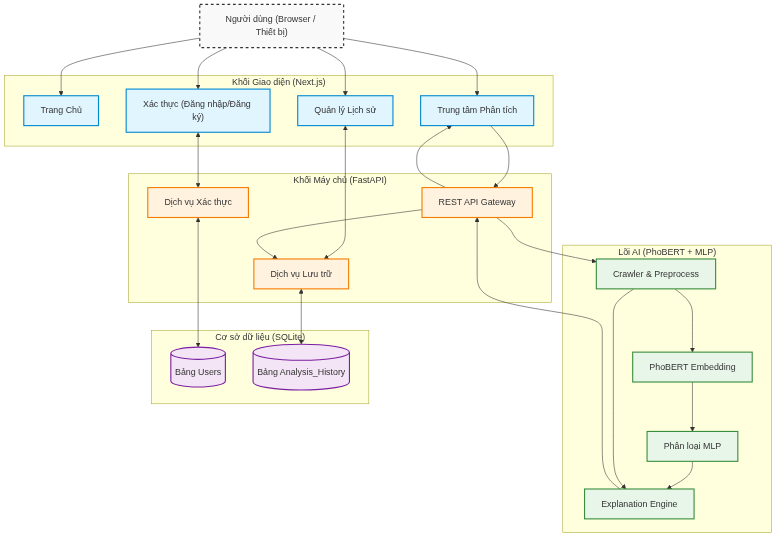
\includegraphics[width=0.95\textwidth]{image/kientruc.png}
    \caption{Sơ đồ Kiến trúc Hệ thống Phân tán}
    \label{fig:kien_truc}
\end{figure}

Như minh họa trong sơ đồ trên, thay vì gộp chung mọi logic xử lý vào một khối nguyên khối (Monolith Architecture), tiểu luận đã áp dụng kiến trúc phân tán \textbf{3 tầng (3-Tier Micro-Architecture) độc lập} (cùng với 1 tầng lưu trữ). Việc chia tách này không chỉ giúp quản lý mã nguồn thuận tiện mà còn đảm bảo tính mở rộng (Scalability), tính tái sử dụng và bảo mật (Security) cho hệ thống trong quá trình triển khai. Sự giao tiếp giữa các tầng được kiểm soát chặt chẽ thông qua các chuẩn HTTP và dữ liệu JSON. Cụ thể, các tầng được thiết kế chi tiết như sau:

\textbf{Tầng 1: Tầng Giao diện Người dùng (Presentation / Client Tier)}

Tầng Giao diện đóng vai trò là điểm chạm đầu tiên (touchpoint) giữa người dùng và hệ thống. Được phát triển trên nền tảng \textbf{Next.js 14} (một React Framework) kết hợp cùng \textbf{Tailwind CSS} và thư viện chuyển động \textbf{Framer Motion}, tầng này đảm bảo trải nghiệm đa nền tảng (Responsive Design) và tương tác ổn định từ màn hình máy tính đến thiết bị di động. Điểm chính trong thiết kế của Tầng Giao diện là nó hoạt động độc lập (agnostic) với các thuật toán Trí tuệ Nhân tạo phức tạp bên dưới. Nhiệm vụ của nó chỉ là tiếp nhận yêu cầu đầu vào từ người dùng (một đoạn văn bản nghi ngờ hoặc một đường dẫn URL bài báo), đóng gói thành các truy vấn chuẩn HTTP RESTful, và gửi đi. Khi nhận được kết quả trả về từ máy chủ, module \textbf{Rõ ràng hóa Dữ liệu} sẽ sử dụng các công cụ vẽ biểu đồ linh hoạt để kết xuất các thông số đánh giá rõ ràng (ví dụ: thanh tiến trình hiển thị 99\% giả mạo, biểu đồ radar cho các chỉ số cảm xúc, hoặc bôi đỏ các từ ngữ giật gân). Cơ chế này giúp người dùng phổ thông, dù không có chuyên môn về máy học, vẫn có thể thuận tiện nắm bắt được kết quả phân loại.

\textbf{Tầng 2: Tầng Xử lý Nghiệp vụ (Application / Backend Tier)}

Đây là "trái tim điều phối" của toàn bộ nền tảng phần mềm, được triển khai bằng framework \textbf{FastAPI}. Các endpoint trả JSON với envelope \texttt{\{"status": "success"|"error", "message": "...", ...\}}; mã HTTP thường là \textbf{200} (kể cả lỗi nghiệp vụ như sai mật khẩu hoặc chưa đăng nhập). Ba phân hệ chính: (1) \textbf{JWT Auth}; (2) \textbf{Web Scraper} (BeautifulSoup khi nhập URL); (3) \textbf{Router} điều phối sang Tầng AI.

\textbf{Tầng 3: Tầng Suy luận Trí tuệ Nhân tạo (AI Inference Tier)}

Tầng này chứa pipeline suy luận ShieldAI: Kiến trúc \textbf{PhoBERT Fine-tuned Sequence Classification} (PyTorch/Transformers) xuất Logits, kết hợp hàm \textbf{Softmax} tính xác suất tin giả; \texttt{verdict.py} quy đổi 3 mức. Sau đó \textbf{ExplanationEngine} (rule-based) quét văn bản gốc (in hoa, dấu câu giật gân…) để sinh JSON giải thích tiếng Việt — \textbf{không} tham gia phân loại.

\textbf{Tầng 4: Tầng Lưu trữ Dữ liệu (Data Storage Tier)}

Mặc dù là tầng thấp nhất, Tầng Lưu trữ lại đóng vai trò tối quan trọng trong việc bảo toàn tính bền vững của nền tảng. Hệ thống sử dụng \textbf{SQLite} kết nối qua mô hình ORM của thư viện SQLAlchemy. Mọi kết quả phân tích JSON chi tiết từ Tầng AI, thông tin tài khoản người dùng, và lịch sử hoạt động đều được lưu vết vĩnh viễn tại đây. Cơ chế này mang lại ưu điểm đáng kể: cho phép người dùng có thể tra cứu ngay lập tức các bài báo họ đã quét trong quá khứ thông qua bảng điều khiển cá nhân (Dashboard), mà không cần phải bắt các cụm GPU/CPU của hệ thống AI phải vất vả chạy lại các phép toán nặng nề cho một dữ liệu cũ.

\secB{3.4.2. Thiết kế cơ sở dữ liệu và Mô hình Thực thể - Mối quan hệ (ERD)}
Để đảm bảo tính bền vững và nhất quán của luồng dữ liệu, hệ thống sử dụng hệ quản trị cơ sở dữ liệu quan hệ (RDBMS) \textbf{SQLite} kết hợp cùng công nghệ ánh xạ đối tượng \textbf{SQLAlchemy ORM (Object-Relational Mapping)}. Việc lựa chọn SQLite được xem là một quyết định kiến trúc chiến lược: nó cung cấp một giải pháp lưu trữ gọn nhẹ (lightweight), không đòi hỏi cấu hình máy chủ cơ sở dữ liệu phức tạp, nhưng vẫn tuân thủ đầy đủ các tiêu chuẩn ACID (Atomicity, Consistency, Isolation, Durability) để đảm bảo an toàn dữ liệu. Thay vì viết các câu lệnh SQL thô (Raw SQL) dễ gây ra lỗ hổng bảo mật SQL Injection, SQLAlchemy ORM cho phép thao tác với dữ liệu dưới dạng các đối tượng (Objects) trong Python, giúp mã nguồn dễ đọc và bảo trì.

Mô hình Thực thể - Mối quan hệ (Entity-Relationship Diagram - ERD) của hệ thống được thiết kế theo hướng tinh gọn, tập trung chủ yếu vào việc giải quyết bài toán chính: lưu trữ định danh người dùng, vết tích của quá trình phân tích AI, và thu thập phản hồi của người dùng để liên tục cải thiện mô hình. Hệ thống bao gồm ba thực thể chính là bảng \texttt{USERS} (Người dùng), bảng \texttt{ANALYSIS\_HISTORY} (Lịch sử phân tích) và bảng \texttt{FEEDBACKS} (Phản hồi).

\begin{figure}[H]
    \centering
    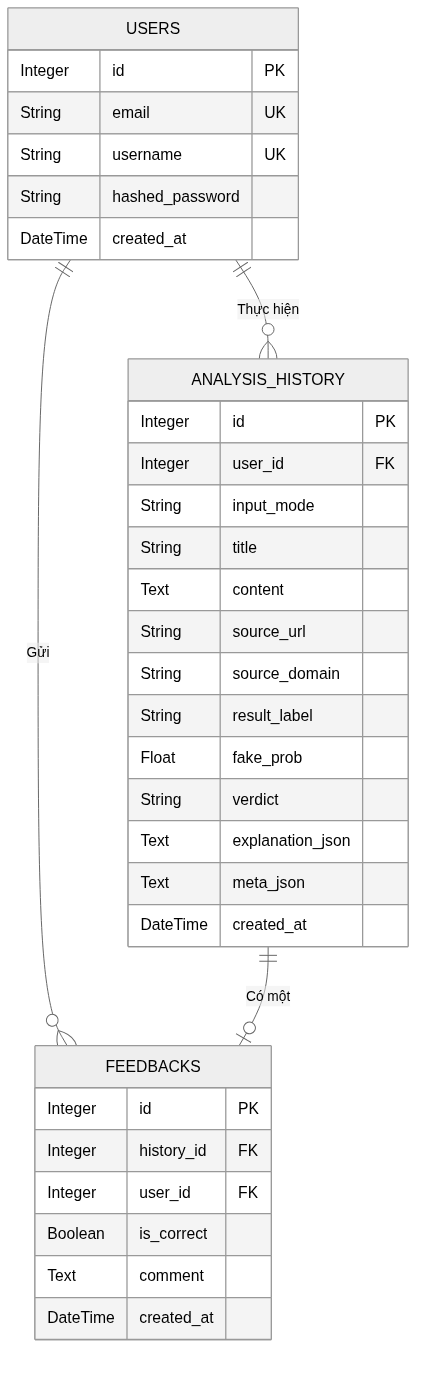
\includegraphics[width=0.95\textwidth]{image/erd.png}
    \caption{Sơ đồ Thực thể - Mối quan hệ (ERD)}
    \label{fig:erd}
\end{figure}

Chi tiết về các bảng và cấu trúc trường (Fields) được phân tích như sau:
\begin{itemize}[label={--},leftmargin=0.75cm,itemsep=3pt]
    \item \textbf{Bảng USERS (Tài khoản người dùng):} Lưu trữ thông tin định danh. Trường \texttt{email} được thiết lập tính duy nhất (UNIQUE) dùng để đăng nhập. Mật khẩu được mã hóa một chiều qua trường \texttt{hashed\_password} nhằm đảm bảo an toàn.
    \item \textbf{Bảng ANALYSIS\_HISTORY (Lịch sử phân tích):} Đóng vai trò lưu vết các thao tác đánh giá tin giả. Bảng lưu trữ nguồn tin (\texttt{url}, \texttt{title}, \texttt{content}), cùng với kết quả trả về từ mô hình bao gồm điểm số tin cậy (\texttt{confidence\_score}) và nhãn cảnh báo (\texttt{verdict}). Mỗi bản ghi được liên kết với một người dùng thông qua khóa ngoại \texttt{user\_id}.
    \item \textbf{Bảng FEEDBACKS (Phản hồi người dùng):} Lưu trữ đánh giá của người dùng về kết quả phân tích. Thuộc tính \texttt{is\_correct} ghi nhận đánh giá đúng/sai từ người dùng, kết hợp với trường \texttt{comments} dạng văn bản. Dữ liệu này hỗ trợ quá trình kiểm chứng và tái huấn luyện mô hình.
\end{itemize}

\begin{table}[H]
\centering
\caption{Từ điển Dữ liệu (Data Dictionary) cho các Thực thể}
\label{tab:data_dictionary}
\begin{tabularx}{\textwidth}{|l|l|l|X|}
\hline
\textbf{Thực thể} & \textbf{Trường dữ liệu} & \textbf{Kiểu dữ liệu} & \textbf{Mô tả chi tiết} \\
\hline
\textbf{USERS} & \texttt{id} & INTEGER & Khóa chính (PK), tự động tăng. \\
\hline
\textbf{USERS} & \texttt{email} & VARCHAR & Email đăng nhập (Unique). \\
\hline
\textbf{USERS} & \texttt{hashed\_password} & VARCHAR & Mật khẩu đã được mã hóa. \\
\hline
\textbf{USERS} & \texttt{created\_at} & DATETIME & Thời điểm khởi tạo tài khoản. \\
\hline
\textbf{ANALYSIS\_HISTORY} & \texttt{id} & INTEGER & Khóa chính (PK), tự động tăng. \\
\hline
\textbf{ANALYSIS\_HISTORY} & \texttt{user\_id} & INTEGER & Khóa ngoại trỏ đến bảng USERS. \\
\hline
\textbf{ANALYSIS\_HISTORY} & \texttt{url} & VARCHAR & Đường dẫn gốc của bài báo (Null). \\
\hline
\textbf{ANALYSIS\_HISTORY} & \texttt{title} & TEXT & Tiêu đề bài báo. \\
\hline
\textbf{ANALYSIS\_HISTORY} & \texttt{content} & TEXT & Nội dung văn bản cần phân tích. \\
\hline
\textbf{ANALYSIS\_HISTORY} & \texttt{confidence\_score} & FLOAT & Điểm số độ tin cậy. \\
\hline
\textbf{ANALYSIS\_HISTORY} & \texttt{verdict} & VARCHAR & Kết quả phân loại (Thật/Giả). \\
\hline
\textbf{ANALYSIS\_HISTORY} & \texttt{created\_at} & DATETIME & Thời gian thực hiện phân tích. \\
\hline
\textbf{FEEDBACKS} & \texttt{id} & INTEGER & Khóa chính (PK), tự động tăng. \\
\hline
\textbf{FEEDBACKS} & \texttt{history\_id} & INTEGER & Khóa ngoại trỏ về ANALYSIS\_HISTORY. \\
\hline
\textbf{FEEDBACKS} & \texttt{is\_correct} & BOOLEAN & Đánh giá dự đoán có chính xác không. \\
\hline
\textbf{FEEDBACKS} & \texttt{comments} & TEXT & Nhận xét chi tiết từ người dùng. \\
\hline
\end{tabularx}
\end{table}

Mối quan hệ giữa các thực thể này là mối quan hệ \textbf{1-N (Một - Nhiều)} giữa người dùng với lịch sử phân tích, và quan hệ \textbf{1-1 (Một - Một)} giữa bản phân tích và một phản hồi duy nhất. Việc ứng dụng ORM SQLAlchemy giúp liên kết tường minh thông qua các khóa ngoại (Foreign Keys). Cấu trúc này phản ánh luồng nghiệp vụ: một người dùng có thể quét nhiều văn bản và gửi các đánh giá phản hồi, toàn bộ dữ liệu này sẽ trở thành nguồn dữ liệu hữu ích để tinh chỉnh và cải thiện mô hình trong tương lai.

\secB{3.4.3. Thiết kế giao diện (UI/UX Design) và Trải nghiệm Người dùng}
Với mục tiêu đưa công nghệ Trí tuệ Nhân tạo phức tạp đến gần hơn với người dùng phổ thông, Giao diện người dùng (User Interface - UI) và Trải nghiệm người dùng (User Experience - UX) của hệ thống được thiết kế theo triết lý \textbf{Tối giản và Được triển khai (Modern Minimalism)}. Toàn bộ nền tảng Frontend được xây dựng bằng Next.js kết hợp với bộ công cụ \textbf{Tailwind CSS}. Việc ứng dụng Tailwind giúp hệ thống duy trì được một cấu trúc mã màu (Color Palette) nhất quán, áp dụng chuẩn thiết kế bo góc (border-radius mềm mại), hiệu ứng kính mờ (Glassmorphism), và đặc biệt là khả năng tương thích hiển thị hiệu quả trên mọi kích thước màn hình (Fully Responsive) từ màn hình Desktop rộng lớn cho đến điện thoại di động. Tổng thể giao diện hệ thống bao gồm ba phân hệ màn hình chính, mỗi phân hệ được thiết kế để giải quyết một điểm chạm cụ thể của người dùng:

\textbf{1. Màn hình Cổng thông tin và Phân tích (Home \& Analysis Portal)}

Đây là màn hình đầu tiên khi người dùng truy cập vào ứng dụng. Thiết kế tập trung sự chú ý của người dùng vào một \textbf{Thanh tìm kiếm (Search Bar)} kích thước lớn đặt ở chính giữa không gian làm việc. Thanh tìm kiếm này được thiết kế tự động với tính năng đa định dạng đầu vào (Multi-input format): người dùng có thể dán (paste) trực tiếp một đường dẫn URL của bài báo mạng, hoặc gõ một đoạn văn bản thô bất kỳ vào khung soạn thảo. Ngay phía dưới là nút "Phân tích nội dung" được tích hợp các hiệu ứng vi mô (micro-interactions) phản hồi xúc giác khi rê chuột (hover). Trong quá trình chờ máy chủ chạy các phép toán AI, màn hình sẽ hiển thị các hiệu ứng tải (Loading animations) dạng sóng ổn định, nhằm cải thiện trải nghiệm người dùng (UX optimization).

\textbf{2. Màn hình Báo cáo Giám định (Result \& Giải thích Heuristic Dashboard)}

Màn hình báo cáo kết quả chính là nơi trình diễn toàn bộ khả năng của công nghệ Trí tuệ Nhân tạo Minh bạch (Heuristic Explanation). Khác với các hệ thống truyền thống chỉ hiện một dòng chữ khô khan, màn hình này áp dụng nguyên lý thiết kế \textbf{Thị giác hóa mức độ rủi ro (Visual Risk Assessment)} thông qua mã màu: \textbf{Màu Đỏ/Cam} sẽ chớp cảnh báo cho các tin giả độc hại và \textbf{Màu Xanh lá cây} sẽ đại diện cho nguồn thông tin an toàn, đáng tin cậy. Giao diện được chia bố cục làm hai vùng chính (Grid Layout):
\begin{itemize}[label={--},leftmargin=0.75cm,itemsep=3pt]
    \item \textbf{Vùng Chỉ số Tổng quan:} Hiển thị một vòng tròn đo lường tỷ lệ phần trăm (Confidence Score) cực lớn, giúp người dùng nắm bắt ngay kết luận cuối cùng (ví dụ: "Bài báo này 94\% là Giả mạo") chỉ trong vòng 2 giây đầu tiên lướt nhìn.
    \item \textbf{Vùng Phân tích Chuyên sâu (Giải thích Heuristic Metrics):} Khu vực này hiển thị các thanh đo (Progress bars) bóc tách chi tiết lý do tại sao văn bản lại bị AI đánh dấu như vậy. Các chỉ số như "Tỷ lệ lạm dụng viết hoa", "Mật độ sử dụng dấu chấm than", "Số lượng từ lóng", hay "Chỉ số cảm xúc tiêu cực" được rõ ràng hóa sinh động. Nhờ tận dụng cấu trúc Component của React, các thanh đồ thị này được thiết lập hiệu ứng chạy ổn định từ 0\% lên đến mức thực tế, cung cấp cho người dùng thông tin chi tiết về các yếu tố ảnh hưởng đến kết quả phân loại.
\end{itemize}

\textbf{3. Màn hình Quản lý Lịch sử (Personal History View)}

Để tăng tính gắn kết cá nhân hóa, hệ thống cung cấp một bảng điều khiển lưu trữ toàn bộ các phiên phân tích trong quá khứ của người dùng. Màn hình này áp dụng thiết kế dạng danh sách thẻ động (Dynamic Cards), cho phép người dùng lướt nhanh qua các tiêu đề bài báo đã quét, thời gian thực hiện thao tác và đóng dấu nhãn Thật/Giả một cách rõ ràng. Điểm phù hợp về mặt UI/UX ở đây là việc triển khai tính năng phân trang (Pagination) ngay tại phía máy chủ kết hợp bộ lọc động, giúp giao diện Frontend có thể tải và cuộn qua hàng trăm bản ghi lịch sử một cách ổn định, quản lý mức sử dụng bộ nhớ (RAM) và hạn chế tình trạng giật lag của trình duyệt.

\secB{3.4.4. Thiết kế thuật toán (PhoBERT Sequence Classification)}
Tiểu luận triển khai kiến trúc \textbf{PhoBERT Fine-tuned Sequence Classification}. Quá trình phân loại diễn ra trực tiếp trên mô hình ngôn ngữ đã được tinh chỉnh; cơ chế giải thích rule-based chạy \textbf{sau} bước phân loại, không can thiệp vào các tensor vector ngữ nghĩa đầu vào. Lưu đồ dưới đây mô tả luồng từ văn bản đầu vào đến verdict và báo cáo giải thích.

\begin{figure}[H]
    \centering
    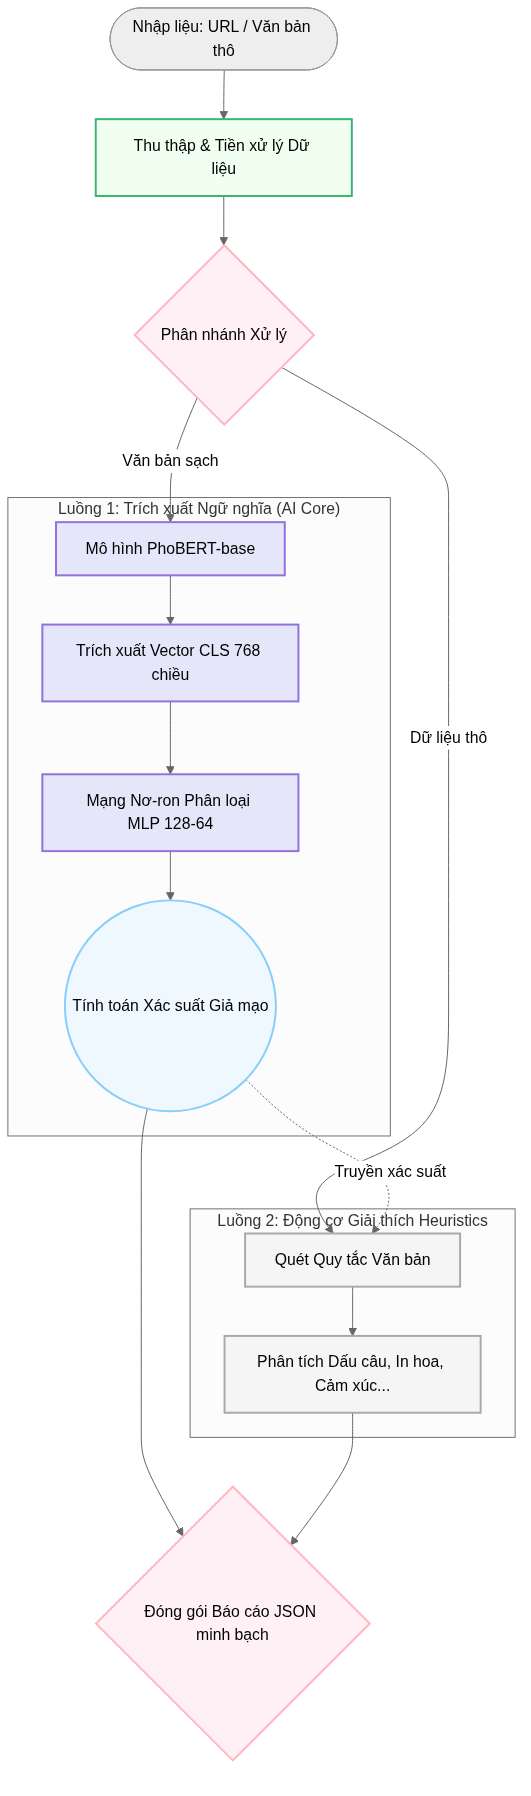
\includegraphics[width=0.95\textwidth]{image/luong_xu_ly.png}
    \caption{Lưu đồ xử lý thuật toán PhoBERT Sequence Classification}
    \label{fig:luong_xu_ly}
\end{figure}

Theo lưu đồ trên, thuật toán chạy theo pipeline tuần tự: tiền xử lý $\rightarrow$ embedding $\rightarrow$ phân loại $\rightarrow$ giải thích. Chi tiết các bước:
\begin{itemize}[label={--},leftmargin=0.75cm,itemsep=3pt]
    \item \textbf{Bước 1: Tiền xử lý (Preprocessing):} Áp dụng \texttt{preprocess\_text}: lowercase $\rightarrow$ xóa URL $\rightarrow$ chuẩn hóa khoảng trắng $\rightarrow$ PyVi tokenize. Cùng logic cho train và inference.
    \item \textbf{Bước 2: Giải mã Ngữ nghĩa (PhoBERT):} Văn bản sạch được đưa qua bộ Tokenizer của PhoBERT để phân tách thành các mảnh từ vựng (Sub-words). Sau đó, chuỗi token này đi qua 12 lớp Mạng Tự chú ý (Self-Attention) của kiến trúc Transformer [6, 7]. Kết quả trả về là một vector đặc trưng đại diện toàn cục cho ngữ cảnh của văn bản (thường gọi là \texttt{[CLS] token vector}), có kích thước \textbf{768 chiều}. Vector này biểu diễn các đặc điểm ngữ nghĩa và cấu trúc ngôn ngữ ẩn chứa trong văn bản.
    \item \textbf{Bước 3: Phân loại (Logits + Softmax):} Mô hình Transformer kiến trúc \texttt{AutoModel}\allowbreak\texttt{For}\allowbreak\texttt{Sequence}\allowbreak\texttt{Classification} xuất ra giá trị Logits, sau đó truyền qua hàm \texttt{Softmax} để tính toán xác suất tin giả; module \texttt{verdict.py} quy đổi thành 3 mức cảnh báo: $<35\%$ tin thật, 35–74\% đáng ngờ, $\ge 75\%$ tin giả.
    \item \textbf{Bước 4: Giải thích (ExplanationEngine):} Module rule-based quét văn bản gốc (viết hoa, dấu chấm than, văn phong giật gân), kết hợp xác suất suy luận để sinh JSON giải thích tiếng Việt.
\end{itemize}

Để minh họa logic lập trình, luồng suy luận được tổng hợp thành đoạn Mã giả (Pseudocode) sau:

\begin{verbatim}
ALGORITHM: PhoBERT Classification & XAI
INPUT:
    T: Văn bản gốc hoặc URL bài viết
OUTPUT:
    Verdict (Tin Thật/Đáng ngờ/Tin Giả), 
    Confidence_Score, 
    Explanation_Report

BEGIN
    // Bước 1: Tiền xử lý (preprocess_text)
    IF T is URL THEN
        T = CRAWL_AND_EXTRACT(T)   // BeautifulSoup
    END IF
    T_clean = PREPROCESS_TEXT(T) // lowercase, xóa URL, PyVi

    // Bước 2: Trích xuất embedding PhoBERT (PyTorch)
    Tokens = PHOBERT_TOKENIZER(T_clean)
    V_phobert = PHOBERT_MODEL(Tokens).extract_CLS() // 768 chiều
    V_scaled = STANDARD_SCALER.transform(V_phobert)

    // Bước 3: Phân loại (AutoModelForSeqClass)
    Logits = PHOBERT_MODEL(Tokens).logits
    Confidence_Score = SOFTMAX(Logits)[1]  // xác suất tin giả

    // Bước 4: Verdict 3 mức (verdict.py)
    Verdict = MAP_TO_VERDICT(Confidence_Score)

    // Bước 5: Giải thích rule-based (ExplanationEngine)
    Explain_Report = EXPLANATION_ENGINE(T, Conf_Score, Verdict)
    // Quét text: viết hoa, dấu câu -> JSON tiếng Việt

    RETURN Verdict, Confidence_Score, Explanation_Report
END
\end{verbatim}

\secA{3.5. Kết luận chương}
Chương 3 đóng vai trò là bản lề định hình toàn bộ khung xương kỹ thuật của tiểu luận, chuyển tiếp từ các lý thuyết nền tảng (Chương 2) sang một bản thiết kế hệ thống phần mềm nguyên mẫu (prototype) và sẵn sàng để lập trình thực tế. Nhìn lại toàn bộ chương, tiểu luận đã giải quyết ba bài toán chính trong việc xây dựng một hệ thống Trí tuệ Nhân tạo ứng dụng thực tiễn:

\textbf{Thứ nhất, về mặt Kiến trúc Phần mềm:} Tiểu luận thiết kế hệ thống theo kiến trúc \textbf{Micro-Architecture 3 tầng (3-Tier) độc lập}. Việc chia tách Tầng Giao diện (Next.js), Tầng Nghiệp vụ (FastAPI) và Tầng Suy luận AI (PhoBERT Sequence Classification) đảm bảo tính bảo mật, khả năng mở rộng và chịu tải trong môi trường mạng thực tế.

\textbf{Thứ hai, về mặt Thiết kế Dữ liệu và Trải nghiệm:} Việc ứng dụng linh hoạt giữa mô hình quan hệ chặt chẽ (SQLite/SQLAlchemy) và định dạng dữ liệu bán cấu trúc (JSON) trong lưu trữ báo cáo Heuristic cho thấy sự linh hoạt về mặt lưu trữ truy vấn. Song song đó, triết lý thiết kế UI/UX được triển khai (Modern Minimalism) với việc thị giác hóa rủi ro qua mã màu góp phần giảm rào cản kỹ thuật, giúp người dùng phổ thông có thể thuận tiện tương tác và nắm bắt các phán quyết của AI.

\textbf{Thứ ba, về mặt Thiết kế Thuật toán Lõi:} Lưu đồ thuật toán tuần tự mô tả pipeline \textbf{PhoBERT Fine-tuned Sequence Classification}: AutoModel\allowbreak For\allowbreak Sequence\allowbreak Classification (Logits) $\rightarrow$ Softmax $\rightarrow$ verdict 3 mức $\rightarrow$ ExplanationEngine rule-based.

Tóm lại, những bản thiết kế logic mạch lạc, từ cấp độ Cơ sở dữ liệu (ERD) cho đến sơ đồ Thuật toán lõi được vạch ra trong Chương 3 chính là kim chỉ nam vững chắc. Khung kiến trúc kỹ thuật này đã sẵn sàng để được chuyển hóa thành những dòng mã nguồn thực tế. Toàn bộ quá trình lập trình cài đặt (Implementation) cũng như chạy các thực nghiệm đánh giá hiệu năng mô hình (Evaluation) sẽ được trình bày cặn kẽ trong \textbf{Chương 4: Hiện thực và Kết quả}.
\newpage

\chap{CHƯƠNG 4: HIỆN THỰC VÀ KẾT QUẢ}
\secA{4.1. Môi trường phát triển và Thực nghiệm}
Để đảm bảo khả năng hiện thực hóa các bản thiết kế kiến trúc phức tạp ở Chương 3, đặc biệt là việc huấn luyện và chạy suy luận (Inference) cho các mô hình Học Sâu (Deep Learning) đòi hỏi khối lượng tính toán lớn, tiểu luận đã được triển khai và kiểm thử trên một môi trường máy tính cục bộ (Local Environment) có cấu hình kỹ thuật tiêu chuẩn. Việc thiết lập môi trường được chia thành hai mảng chuyên biệt: Phần cứng và Phần mềm.

\secB{4.1.1. Môi trường Phần cứng (Hardware Environment)}
Quá trình huấn luyện mạng nơ-ron đa lớp và kiến trúc Transformer [6, 7] (PhoBERT) yêu cầu khả năng tính toán khối lượng lớn ma trận, điều mà các bộ vi xử lý thông thường khó đáp ứng hiệu quả trong thời gian ngắn. Do đó, hệ thống phần cứng được thiết lập với các thông số sau:
\begin{itemize}[label={--},leftmargin=0.75cm,itemsep=3pt]
    \item \textbf{Vi xử lý trung tâm (CPU):} Tối thiểu Intel Core i5 hoặc AMD Ryzen 5 thế hệ mới, đáp ứng tốt quá trình cào dữ liệu (Web Scraping) đa luồng bằng BeautifulSoup và xử lý tiền dữ liệu văn bản bằng Regex.
    \item \textbf{Bộ nhớ trong (RAM):} Tối thiểu \textbf{16GB}. Dung lượng này là ranh giới bắt buộc để hệ thống có thể tải đồng thời tập dữ liệu huấn luyện (Dataset) vào bộ nhớ chính, đồng thời duy trì các máy chủ ảo cục bộ (cả FastAPI và Next.js) hoạt động song song mà không bị hiện tượng tràn RAM (Out-of-memory crash).
    \item \textbf{Bộ xử lý Đồ họa (GPU):} Khuyến nghị card \textbf{NVIDIA} có hỗ trợ \textbf{CUDA} để tăng tốc quá trình suy luận PhoBERT (embedding). Quá trình tinh chỉnh (Fine-tuning) PhoBERT yêu cầu tài nguyên GPU đủ lớn để tính toán và cập nhật trọng số hiệu quả.
\end{itemize}

\secB{4.1.2. Môi trường Hệ điều hành và Phần mềm}
Để tạo ra một nền tảng vận hành ổn định, hạn chế rủi ro xung đột thư viện (Dependency conflicts) thường gặp trong quá trình biên dịch mô hình AI, tiểu luận sử dụng các phiên bản phần mềm chính như sau:
\begin{itemize}[label={--},leftmargin=0.75cm,itemsep=3pt]
    \item \textbf{Hệ điều hành chính:} \textbf{Linux (Ubuntu)} — tương thích mã nguồn mở, khởi chạy script điều phối (\texttt{setup.sh}, \texttt{run.sh}) ổn định.
    \item \textbf{Hệ sinh thái Backend \& AI:} 
    \begin{itemize}[label={--},leftmargin=0.75cm,itemsep=3pt]
        \item \textbf{Ngôn ngữ:} Sử dụng phiên bản \texttt{Python 3.10+} (toàn bộ mã nguồn chạy bên trong một môi trường ảo Virtual Environment riêng biệt để cách ly các thư viện).
        \item \textbf{Framework máy chủ:} \texttt{FastAPI} kết hợp cùng máy chủ ASGI \texttt{Uvicorn} để kích hoạt khả năng xử lý bất đồng bộ (Asynchronous) ở tốc độ cao nhất.
        \item \textbf{Thư viện AI Lõi:} \texttt{PyTorch}, \texttt{Transformers}, \texttt{Scikit-learn}.
    \end{itemize}
    \item \textbf{Hệ sinh thái Frontend:} Được xây dựng trên nền tảng môi trường cục bộ \textit{Node.js}. Sử dụng ngôn ngữ \textit{TypeScript} nhằm ép buộc tính an toàn kiểu dữ liệu (Type-safety). Khung thiết kế chính là \textit{Next.js 14} kết hợp với hệ sinh thái \textit{React} và bộ thư viện tiện ích \textit{Tailwind CSS}.
    \item \textbf{Hệ quản trị Cơ sở dữ liệu:} Để phục vụ mục đích thực nghiệm và phát triển (Development Phase) linh hoạt, tiểu luận triển khai CSDL \texttt{SQLite} thay vì cài đặt các hệ thống máy chủ cồng kềnh như MySQL hay PostgreSQL. Mọi giao tiếp nhúng với CSDL được thực hiện gián tiếp thông qua thư viện ORM \texttt{SQLAlchemy}.
\end{itemize}

\secA{4.2. Quá trình hiện thực}
\secB{4.2.1. Cài đặt các module lõi của hệ thống (Core Modules Implementation)}
Mã nguồn của hệ thống được tổ chức khoa học theo nguyên tắc \textbf{Separation of Concerns (Tách biệt mối quan tâm)}. Thay vì gộp chung toàn bộ logic vào một khối lệnh nguyên khối khó kiểm soát, tiểu luận đã phân rã hệ thống thành các module Python độc lập. Lối kiến trúc này giúp mã nguồn dễ bảo trì, dễ kiểm thử (Unit Test) và thuận tiện nâng cấp thuật toán trong tương lai. Các module lõi được cài đặt như sau:

\begin{itemize}[label={--},leftmargin=0.75cm,itemsep=3pt]
    \item \textbf{Thu thập và Tiền xử lý:} Khi nhập URL, lấy tiêu đề và nội dung HTML. Văn bản thu được đi qua hàm tiền xử lý. Module làm sạch chỉ dùng cho kiểm thử.
    \item \textbf{Suy luận Phân loại:} Tải mô hình PhoBERT-base qua \texttt{Transformers}, trích xuất vector [CLS] 768 chiều, tiến hành suy luận bằng \texttt{AutoModelFor}\allowbreak\texttt{Sequence}\allowbreak\texttt{Classification}. Mảng Logits đi qua \texttt{Softmax} tính xác suất tin giả; sau đó quy đổi thành 3 mức cảnh báo qua \texttt{verdict.py}.
    \item \textbf{Module Giải thích (\texttt{explanation\_engine.py}):} Chạy sau phân loại. Quét văn bản gốc (tỷ lệ IN HOA, dấu câu, văn phong giật gân), áp luật rule-based và sinh JSON giải thích tiếng Việt — không tham gia vector đầu vào của mô hình.
\end{itemize}

\secB{4.2.2. Dữ liệu nghiên cứu và Quy trình Tiền xử lý}
\textbf{Giới thiệu bộ dữ liệu (Dataset Overview)}

Để quá trình Tinh chỉnh (Fine-tuning) mang lại khả năng tổng quát hóa cao và độ chính xác lớn nhất trong thực tế, tiểu luận sử dụng dữ liệu được gộp thành từ 4 bộ ngữ liệu (dataset) uy tín trên nền tảng Kaggle. Tổng hợp lại, tập dữ liệu lớn mang đến sự đa dạng về văn phong và chủ đề, bao gồm:
\begin{itemize}[label={--},leftmargin=0.75cm,itemsep=3pt]
    \item \textbf{Bộ 1 (phngnguynthu1803):} Cung cấp dữ liệu tin tức thật đa dạng nhằm cân bằng tập huấn luyện, giúp mô hình học được ngôn ngữ báo chí chính thống.
    \item \textbf{Bộ 2 (chuynvinquc):} Bao gồm các bài đăng từ mạng xã hội và tin tức tổng hợp, giúp hệ thống kháng nhiễu với văn phong lóng mạng.
    \item \textbf{Bộ 3 (goumanguyen):} Cung cấp các cặp văn bản được gán nhãn rõ ràng phục vụ cho việc kiểm chứng thông tin tổng hợp.
    \item \textbf{Bộ 4 (leviettrieu369):} Bộ dữ liệu chuyên biệt về tin giả y tế/sức khỏe bằng tiếng Việt thời kỳ COVID-19. Đây là bộ lõi giúp mô hình nhạy bén với các thuật ngữ sức khỏe và tin đồn y khoa độc hại.
\end{itemize}
Tất cả dữ liệu từ 4 nguồn này được tự động thu thập, hợp nhất và đi qua cùng một pipeline tiền xử lý chung (loại bỏ bài viết dưới 20 ký tự, khử nhiễu HTML, v.v.), đem lại quy mô \textbf{hơn 22.000 mẫu tin}, cung cấp cho mô hình khả năng nhận diện các thủ thuật lừa đảo đa dạng và tinh vi trên không gian mạng.

\textbf{Biện luận lý do lựa chọn bộ dữ liệu quy mô lớn}

Việc quyết định sử dụng bộ dữ liệu đa lĩnh vực này xuất phát từ ba luận điểm mang tính chiến lược:
\begin{itemize}[label={--},leftmargin=0.75cm,itemsep=3pt]
    \item \textbf{Tính khái quát hóa cao (Generalization):} Khác với các hệ thống chỉ học trên một miền dữ liệu hẹp, việc học trên \textbf{hơn 22.000 mẫu} tin tổng hợp giúp mô hình nắm bắt ngữ cảnh chuyên ngành và có thể áp dụng kiểm chứng thông tin sức khỏe trên không gian mạng.
    \item \textbf{Độ phong phú của thuật ngữ:} Ngữ liệu lớn chứa rất nhiều từ vựng đan xen với cấu trúc câu mang tính mồi chài của giới bán hàng giả hoặc câu view giật gân. Đây là một môi trường thử nghiệm phù hợp để mô hình PhoBERT [1] học cách phân biệt ngữ cảnh tiếng Việt phức tạp.
    \item \textbf{Sự phù hợp với phương pháp Heuristics:} Các tin giả trên không gian mạng thường xuất hiện các dạng mẫu hành vi nhất định (như viết hoa toàn bộ tựa đề, lạm dụng dấu chấm than). Do đó, tập dữ liệu này cung cấp cơ sở thực nghiệm phù hợp để Động cơ Giải thích Heuristics phân tích và trích xuất các dấu hiệu bất thường.
\end{itemize}

\textbf{Quy trình Hợp nhất và Tiền xử lý Dữ liệu Huấn luyện (Data Merging \& Preprocessing Workflow)}

Do dữ liệu có nguồn gốc từ 4 tập khác biệt nhau về mặt cấu trúc (tên cột khác nhau như \texttt{content}, \texttt{post\_message}, \texttt{Maintext}), tiểu luận đã xây dựng một tiến trình hợp nhất (Merging Pipeline) và tiền xử lý thống nhất như Hình \ref{fig:data_merge}:

\begin{figure}[H]
    \centering
    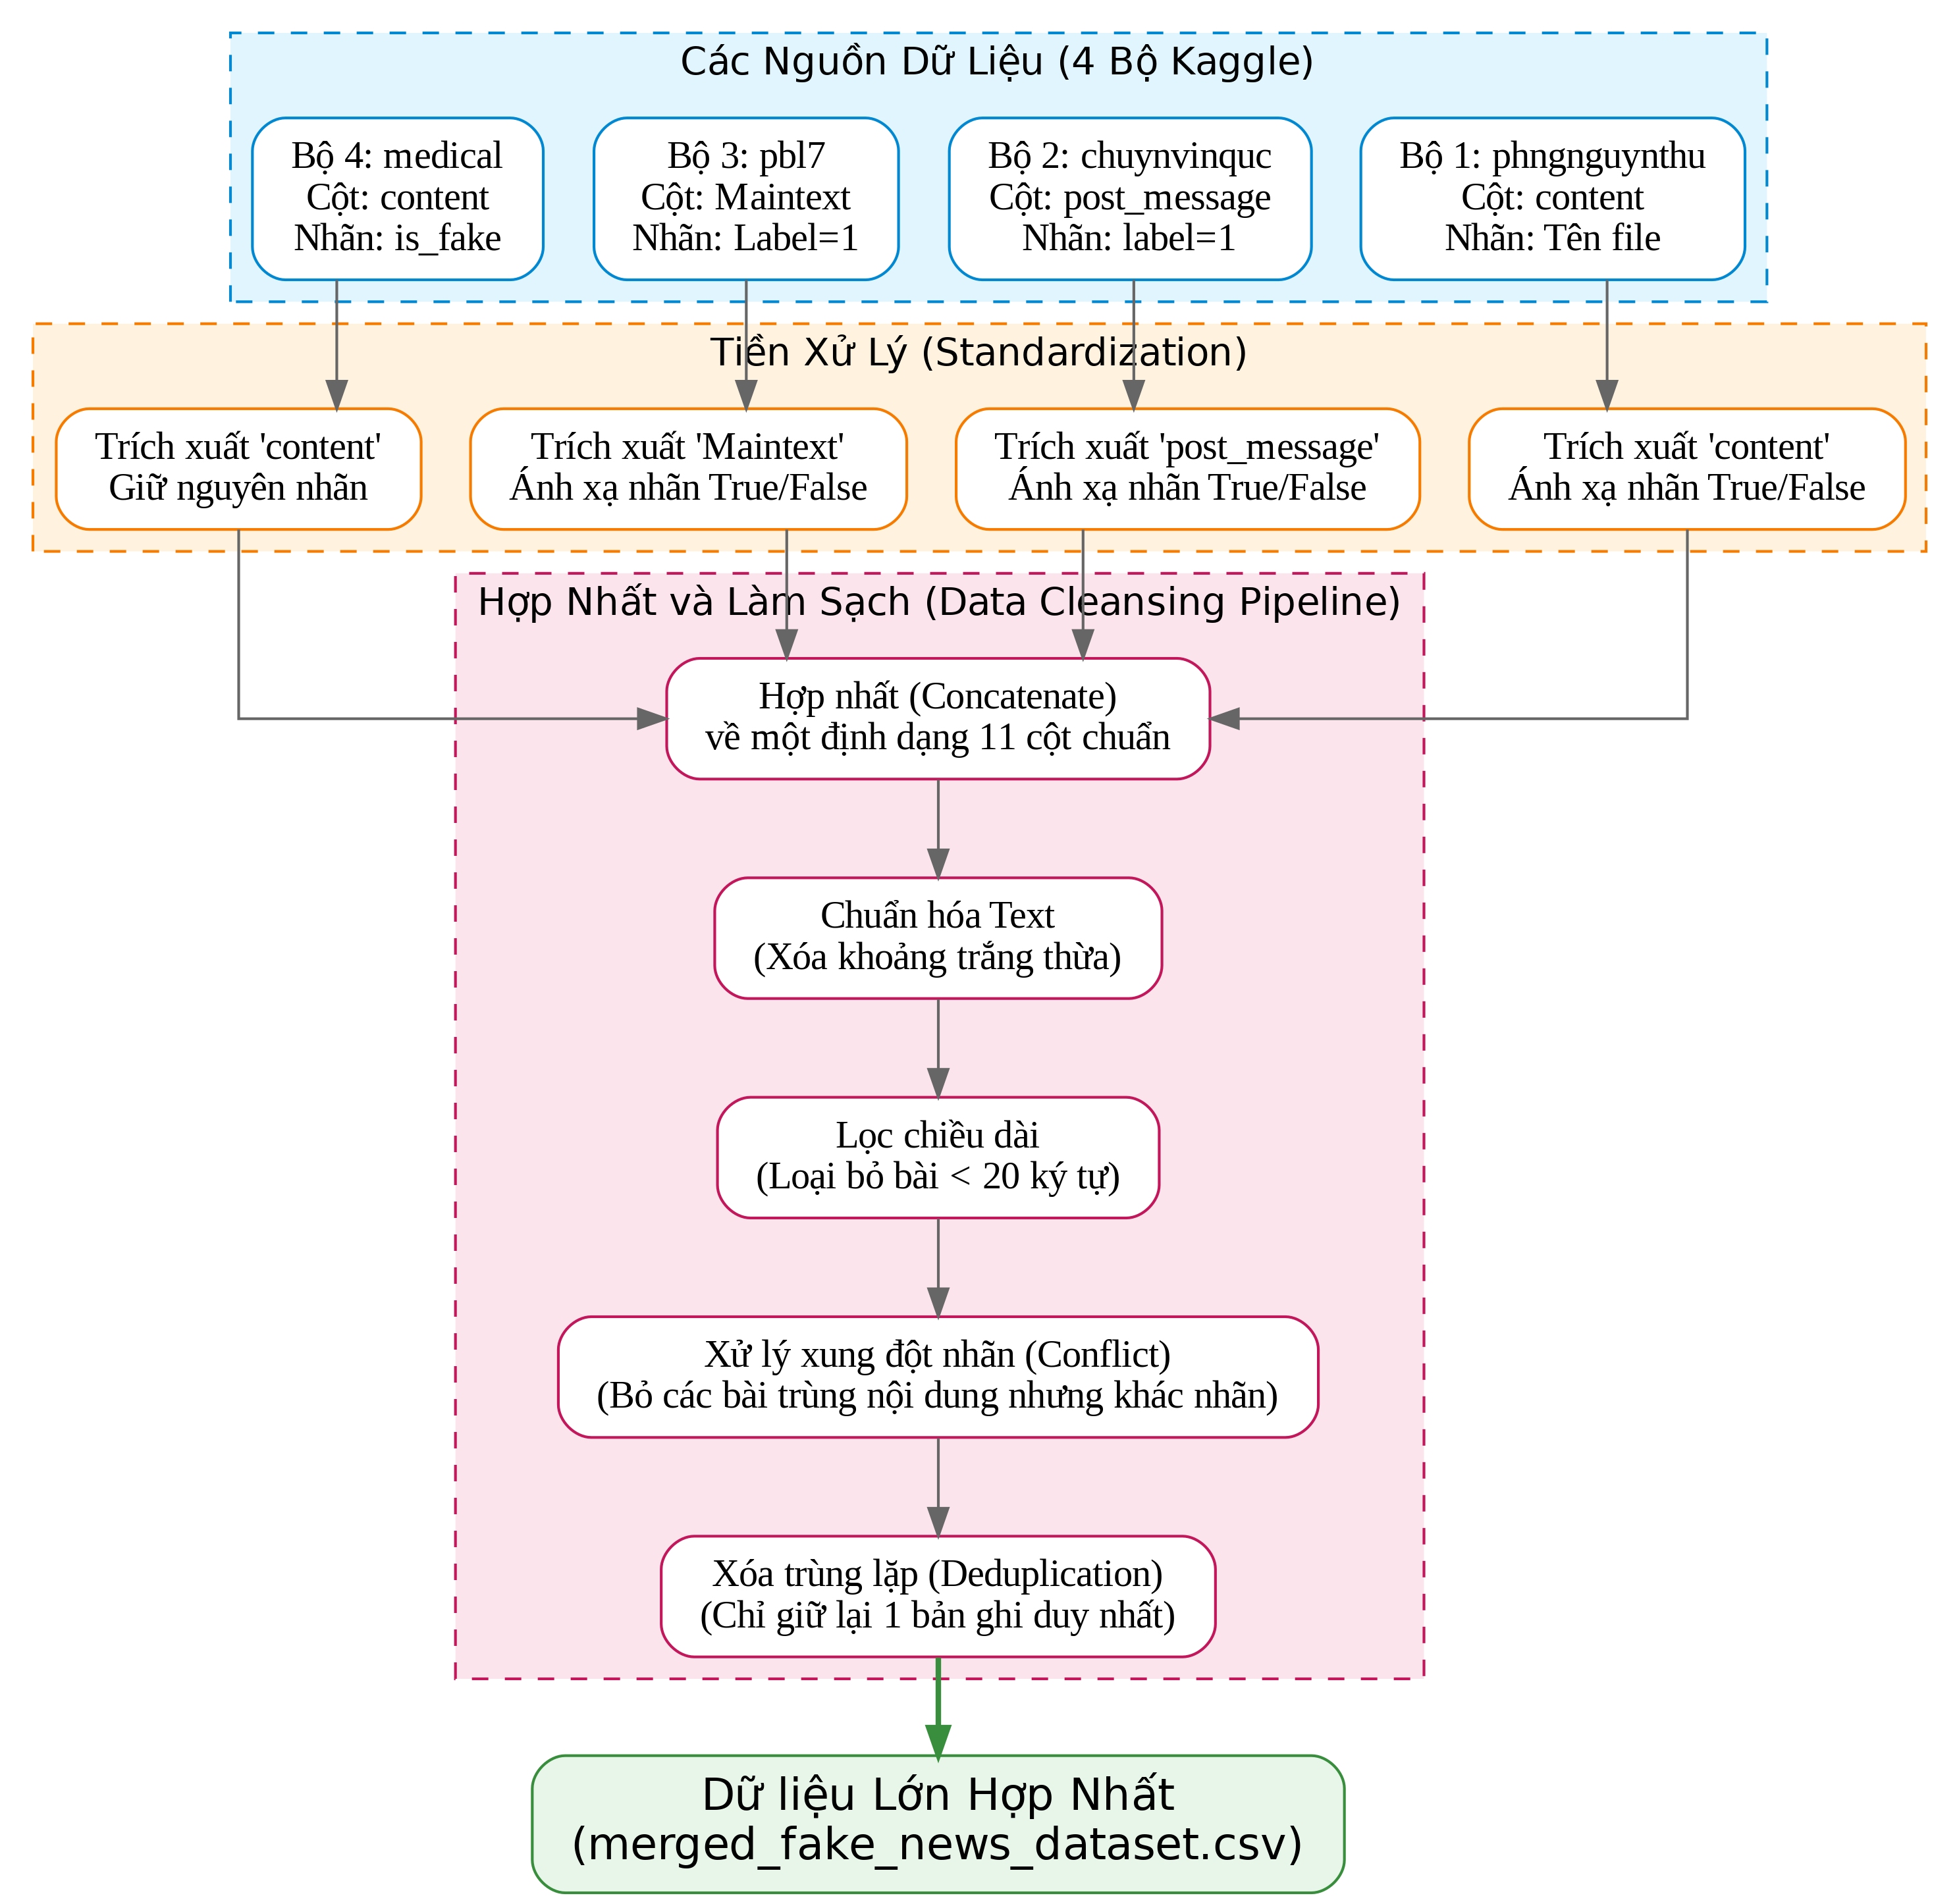
\includegraphics[width=0.95\textwidth]{image/luong_gop_du_lieu.png}
    \caption{Sơ đồ thuật toán gộp và làm sạch 4 bộ dữ liệu thành Data Pipeline hợp nhất}
    \label{fig:data_merge}
\end{figure}

\begin{itemize}[label={--},leftmargin=0.75cm,itemsep=3pt]
    \item \textbf{Đồng bộ hóa Trường dữ liệu (Schema Mapping):} Tự động ánh xạ nội dung từ các cột văn bản khác nhau về chung một cột \texttt{content}. Nhãn phân loại từ các định dạng boolean/string khác nhau được ánh xạ chuẩn xác về biến \texttt{is\_fake} (True/False).
    \item \textbf{Làm sạch và Lọc chiều dài (Normalization \& Filtering):} Loại bỏ khoảng trắng thừa và vứt bỏ toàn bộ các bản ghi có chiều dài nội dung dưới 20 ký tự để loại trừ nhiễu (noise).
    \item \textbf{Xử lý Xung đột và Xóa trùng lặp (Conflict Resolution \& Deduplication):} Nếu phát hiện các bài báo có nội dung giống hệt nhau nhưng mang nhãn (Thật/Giả) trái ngược nhau từ các nguồn khác nhau, hệ thống sẽ loại bỏ các bản ghi xung đột này. Cuối cùng, hàm \texttt{drop\_duplicates()} được sử dụng để loại bỏ các bản ghi bị trùng lặp, đảm bảo không có bất kỳ bài báo nào xuất hiện 2 lần trên toàn hệ thống (Triệt tiêu rủi ro Data Leakage). Kết quả thu về \textbf{hơn 22.000 mẫu} dữ liệu có chất lượng đồng nhất hơn.
    \item \textbf{Tách tập huấn luyện (Train/Val/Test Split):} Chia tỷ lệ \textbf{76\% Huấn luyện (17.201 mẫu) — 12\% Xác thực (2.716 mẫu) — 12\% Kiểm thử (2.716 mẫu)}, sử dụng kỹ thuật chia tách phân tầng (Stratified Split) với \texttt{random\_state=42} để đảm bảo tỷ lệ Thật/Giả luôn đồng đều trên cả 3 tập.
    \item \textbf{Huấn luyện Fine-tuning:} Dữ liệu được mã hóa bằng \texttt{AutoTokenizer} của PhoBERT trước khi được nạp vào mô hình \texttt{AutoModel\allowbreak For\allowbreak Sequence\allowbreak Classification}. Quá trình huấn luyện không sử dụng tái lấy mẫu (resampling) do tập dữ liệu đã tương đối cân bằng.
\end{itemize}

\secB{4.2.3. Tổ chức cấu trúc mã nguồn (Project Directory Structure)}
Để đảm bảo tính mở rộng, dễ bảo trì và làm việc nhóm hiệu quả, toàn bộ mã nguồn của dự án được tổ chức chặt chẽ theo mô hình phân tách (Decoupled). Dưới đây là sơ đồ cây thư mục (Directory Tree) minh họa cấu trúc các thành phần chính của hệ thống ShieldAI:

{\footnotesize
\begin{verbatim}
ShieldAI_Project/
├── backend/                  # Khối Máy chủ API (Python & FastAPI)
│   ├── api/                  # Các API Endpoints (Auth, Analyze, History)
│   ├── auth/                 # Xử lý bảo mật, mã hóa JWT bằng bcrypt
│   ├── database/             # Kết nối SQLite và quản lý Models (SQLAlchemy)
│   ├── experiments/          # Lưu trữ biểu đồ đánh giá
│   ├── models/               # Thư mục lưu trữ mô hình AI
│   │   └── phobert-fakenews-final/ # Sequence Classification Model
│   ├── tests/                # Bộ 38 kịch bản kiểm thử (Pytest) [14]
│   ├── training/             # Tiền xử lý, hợp nhất dữ liệu và Fine-tune
│   ├── data_crawler.py       # Thu thập dữ liệu báo chí từ URL
│   ├── explanation_engine.py # Sinh báo cáo giải thích Rule-based
│   ├── text_utils.py         # Tiền xử lý văn bản bằng PyVi
│   ├── phobert_inference.py  # Đóng gói kiến trúc suy luận PhoBERT
│   └── main.py               # Điểm khởi chạy của máy chủ FastAPI
├── docs/                     # Tài liệu kỹ thuật, Hướng dẫn
├── frontend/                 # Khối Giao diện Người dùng (Next.js)
│   ├── app/                  # Kiến trúc App Router Next.js
│   ├── components/           # Components tái sử dụng (Navbar, Chart, Hero)
│   ├── context/              # Quản lý trạng thái (React Context API)
│   ├── lib/                  # Tiện ích gọi API (Axios)
│   └── tailwind.config.ts    # Cấu hình Design System
├── scripts/                  # Bash script hỗ trợ chạy dự án
├── run.sh                    # Script tiện ích chạy Backend và Frontend
├── README.md                 # Tài liệu tổng quan
└── requirements.txt          # Danh sách thư viện Python
\end{verbatim}
}

Mô hình tổ chức này tuân thủ nguyên tắc \textit{Separation of Concerns} (Tách biệt mối quan tâm), giúp đội ngũ phát triển thuận tiện khoanh vùng lỗi, thực hiện kiểm thử độc lập ở Backend mà không ảnh hưởng tới quá trình thiết kế UI/UX ở Frontend.

\secA{4.3. Kết quả đạt được}
\secB{4.3.1. Kết quả giao diện ứng dụng (User Interface Implementation)}
Hệ thống đã được lập trình bằng Next.js và triển khai thành công trên môi trường cục bộ. Giao diện thực tế hoạt động ổn định, đáp ứng chính xác các yêu cầu về thiết kế UI/UX đã đề ra ở Chương 3. Dưới đây là các minh chứng hình ảnh chụp lại từ hệ thống thực tế đang vận hành:

\begin{figure}[H]
    \centering
    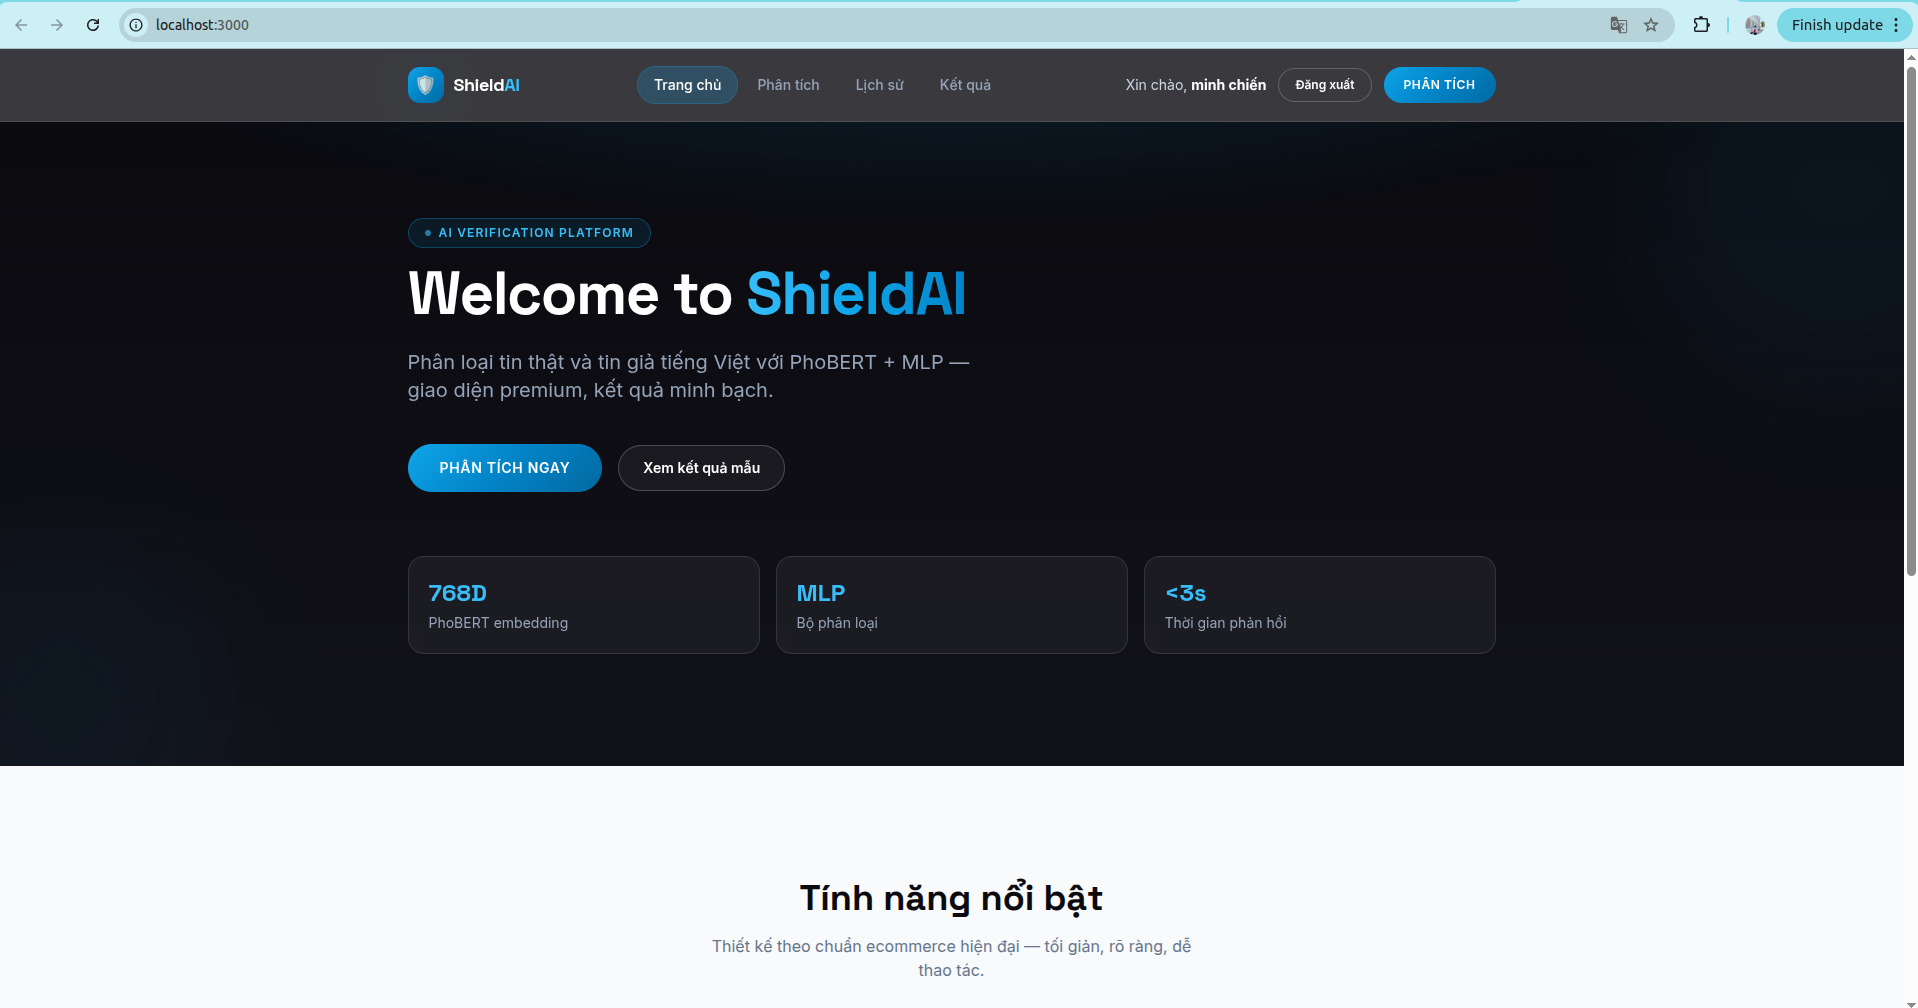
\includegraphics[width=0.95\textwidth]{image/1_TrangChu.png}
    \caption{Giao diện màn hình Cổng thông tin (Home) với thiết kế tối giản}
    \label{fig:trang_chu}
\end{figure}

\begin{figure}[H]
    \centering
    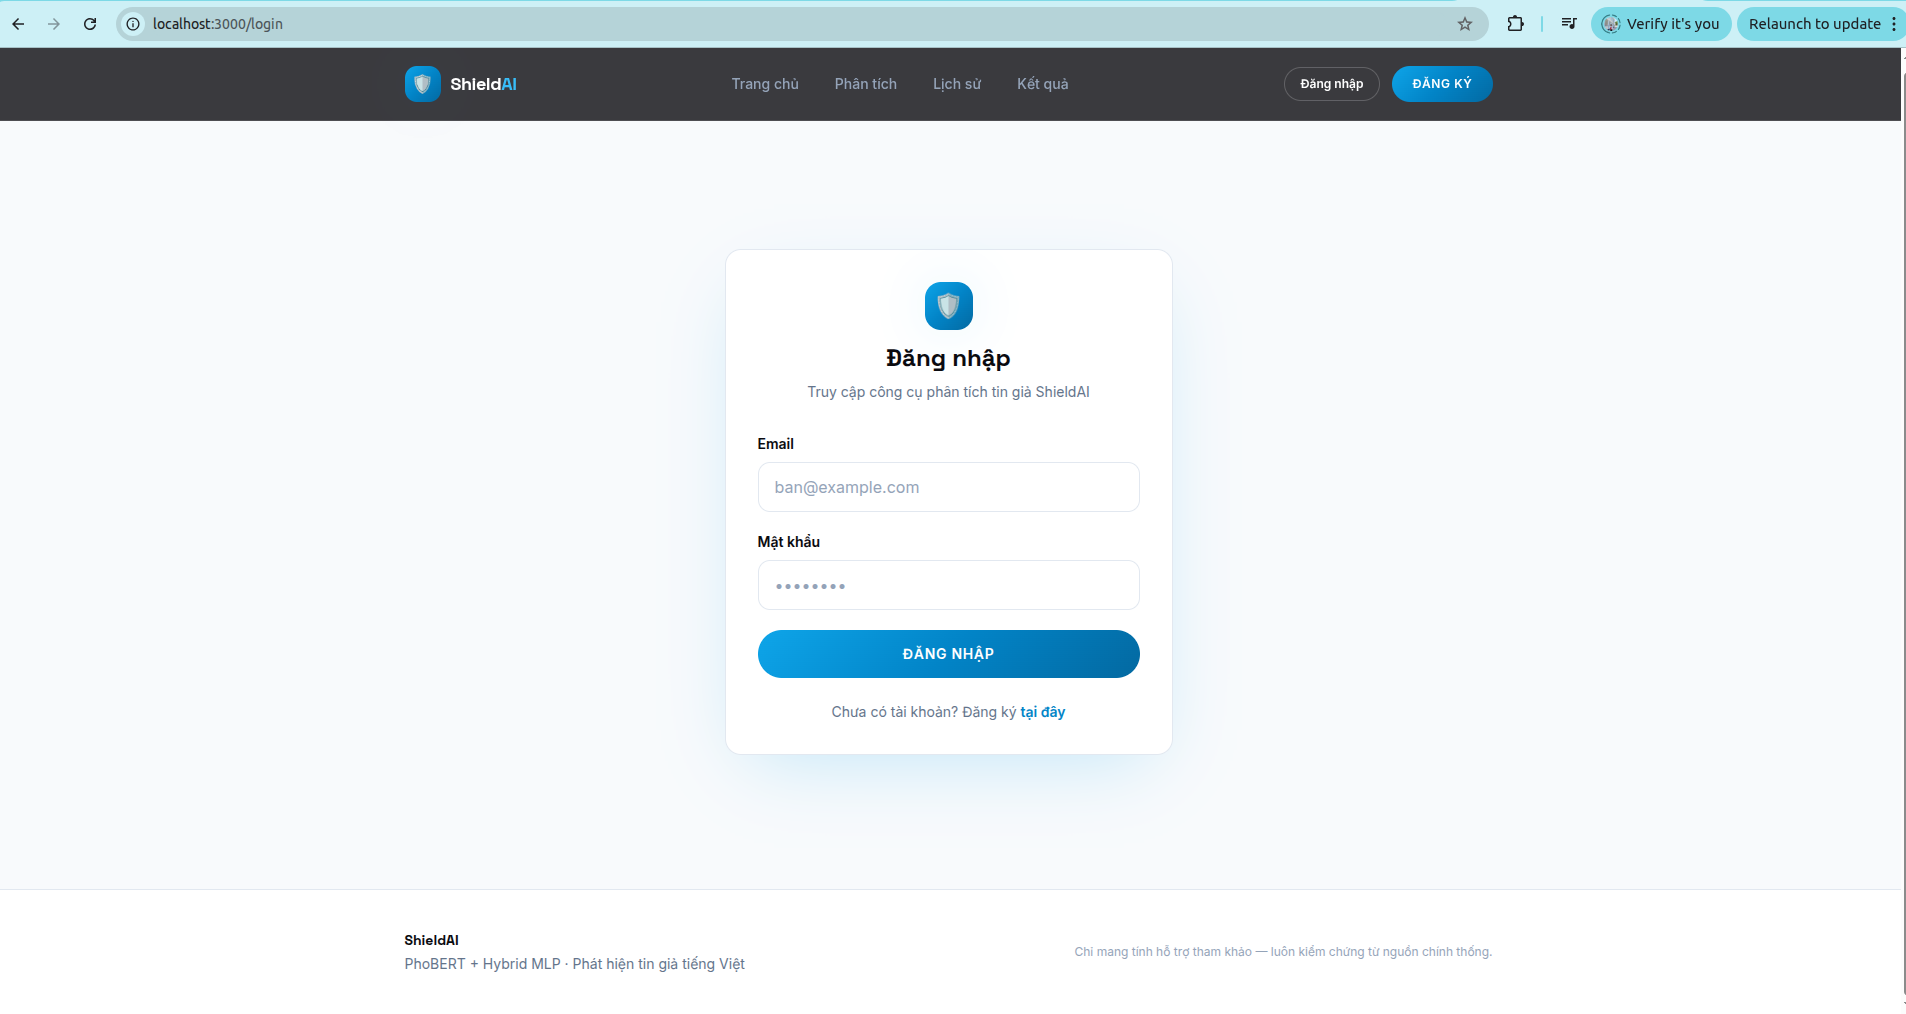
\includegraphics[width=0.95\textwidth]{image/2_TrangDangNhap.png}
    \caption{Giao diện Đăng nhập (Authentication) bảo mật người dùng}
    \label{fig:dang_nhap}
\end{figure}

\begin{figure}[H]
    \centering
    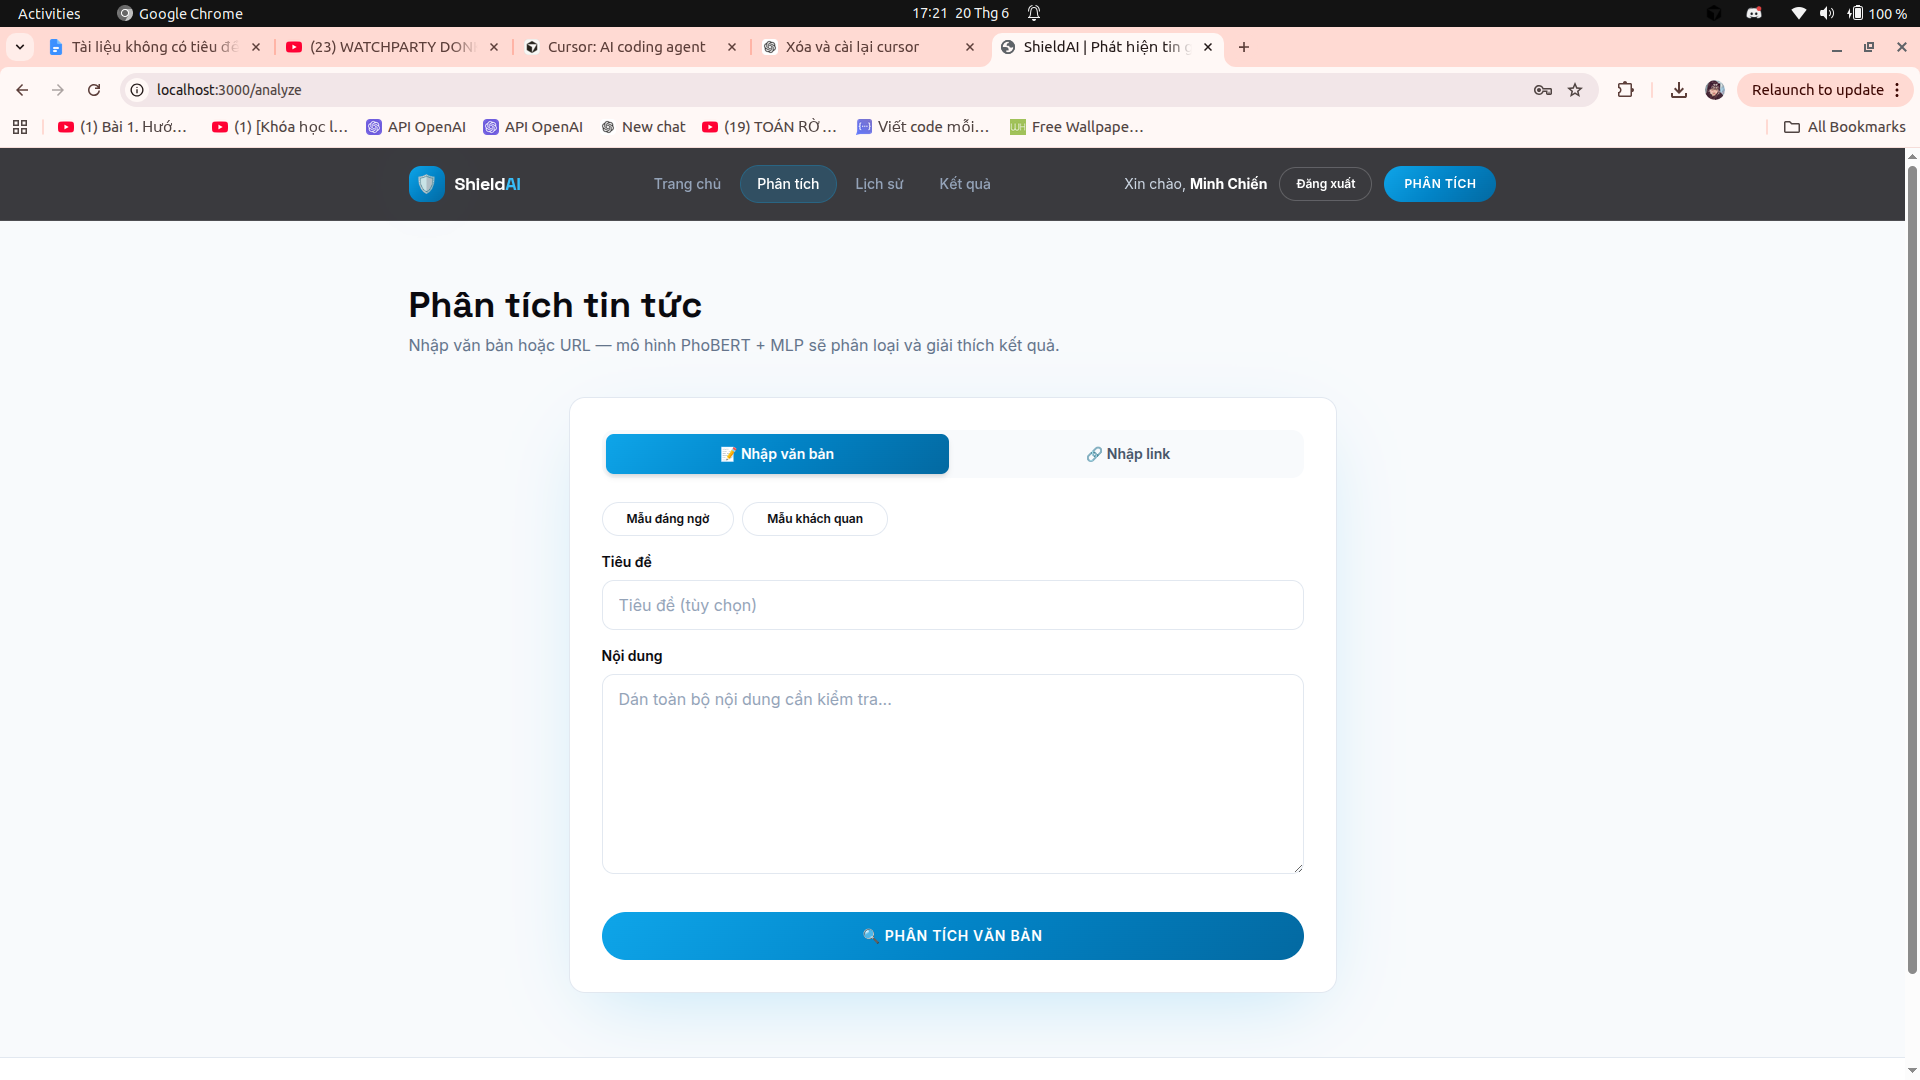
\includegraphics[width=0.95\textwidth]{image/01_Giao_dien_Nhap_Van_Ban.png}
    \caption{Giao diện trung tâm Phân tích — Hỗ trợ nhập văn bản trực tiếp}
    \label{fig:nhap_van_ban}
\end{figure}

\begin{figure}[H]
    \centering
    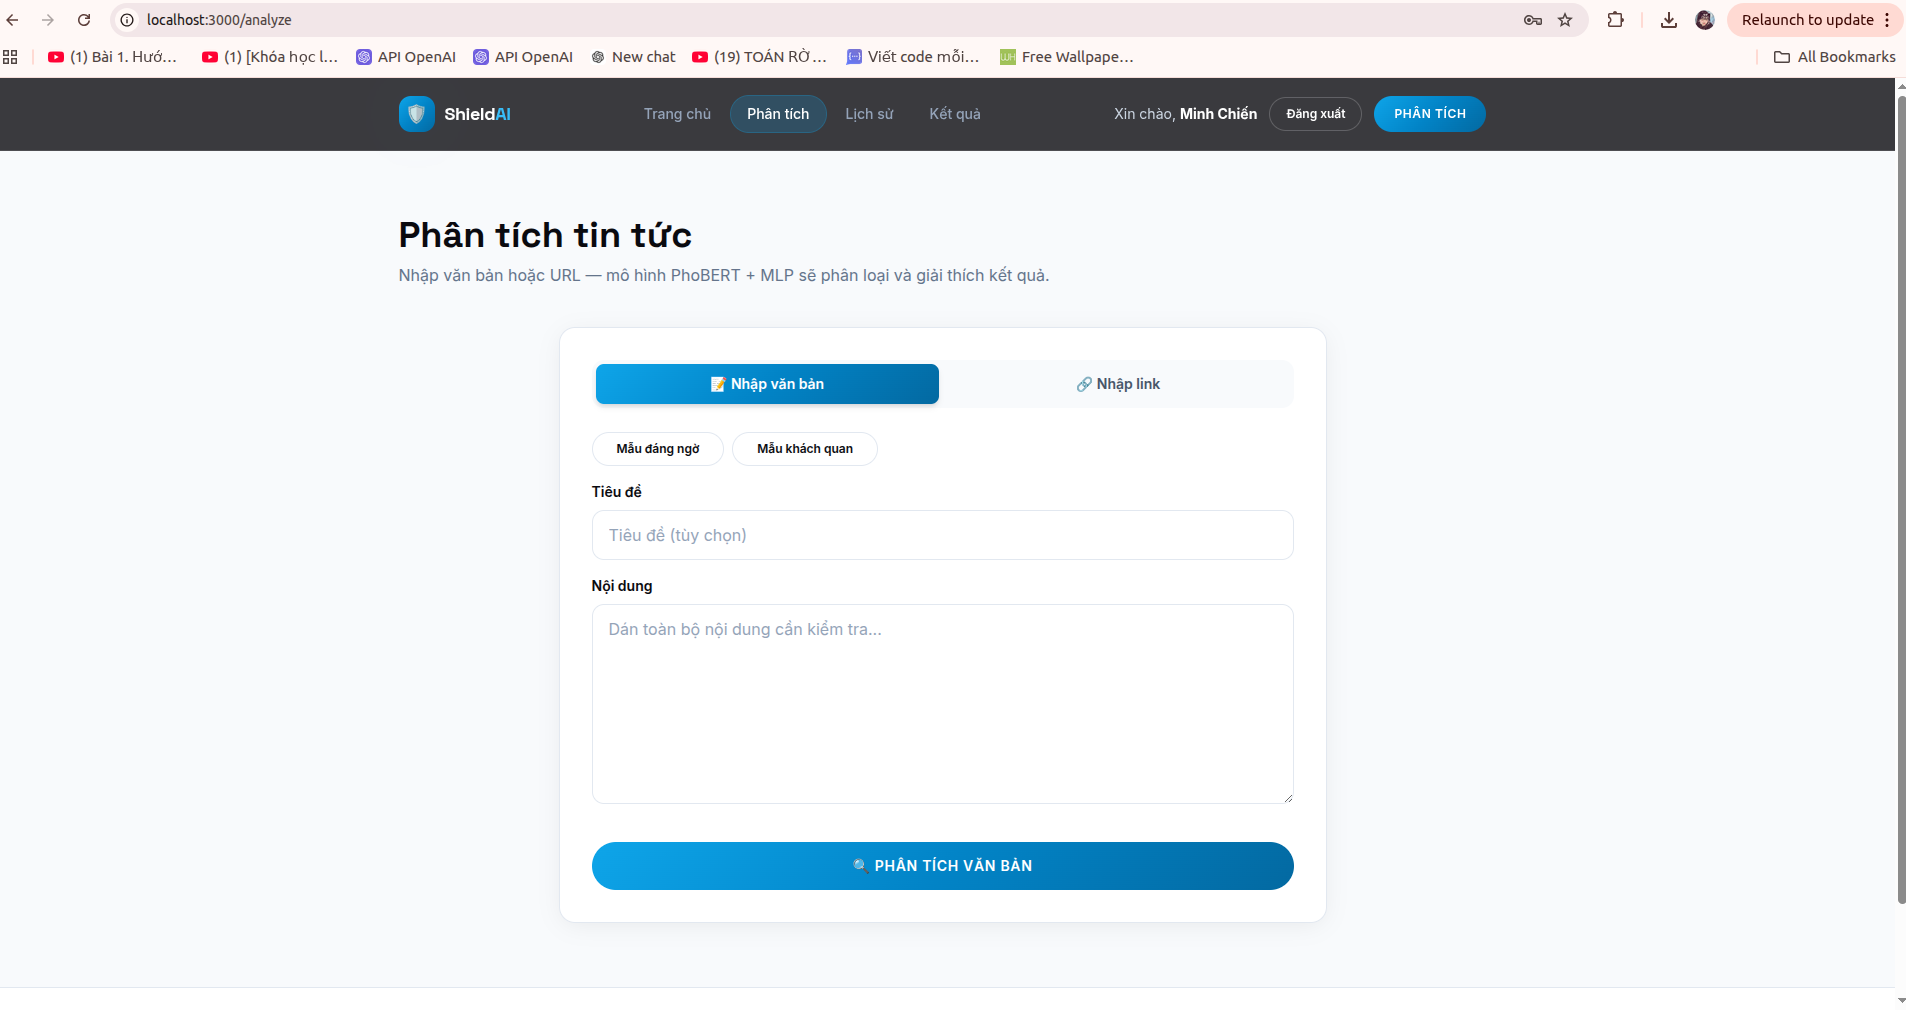
\includegraphics[width=0.95\textwidth]{image/03_Giao_dien_Nhap_Link.png}
    \caption{Giao diện trung tâm Phân tích — Hỗ trợ dán liên kết (URL)}
    \label{fig:nhap_link}
\end{figure}

\begin{figure}[H]
    \centering
    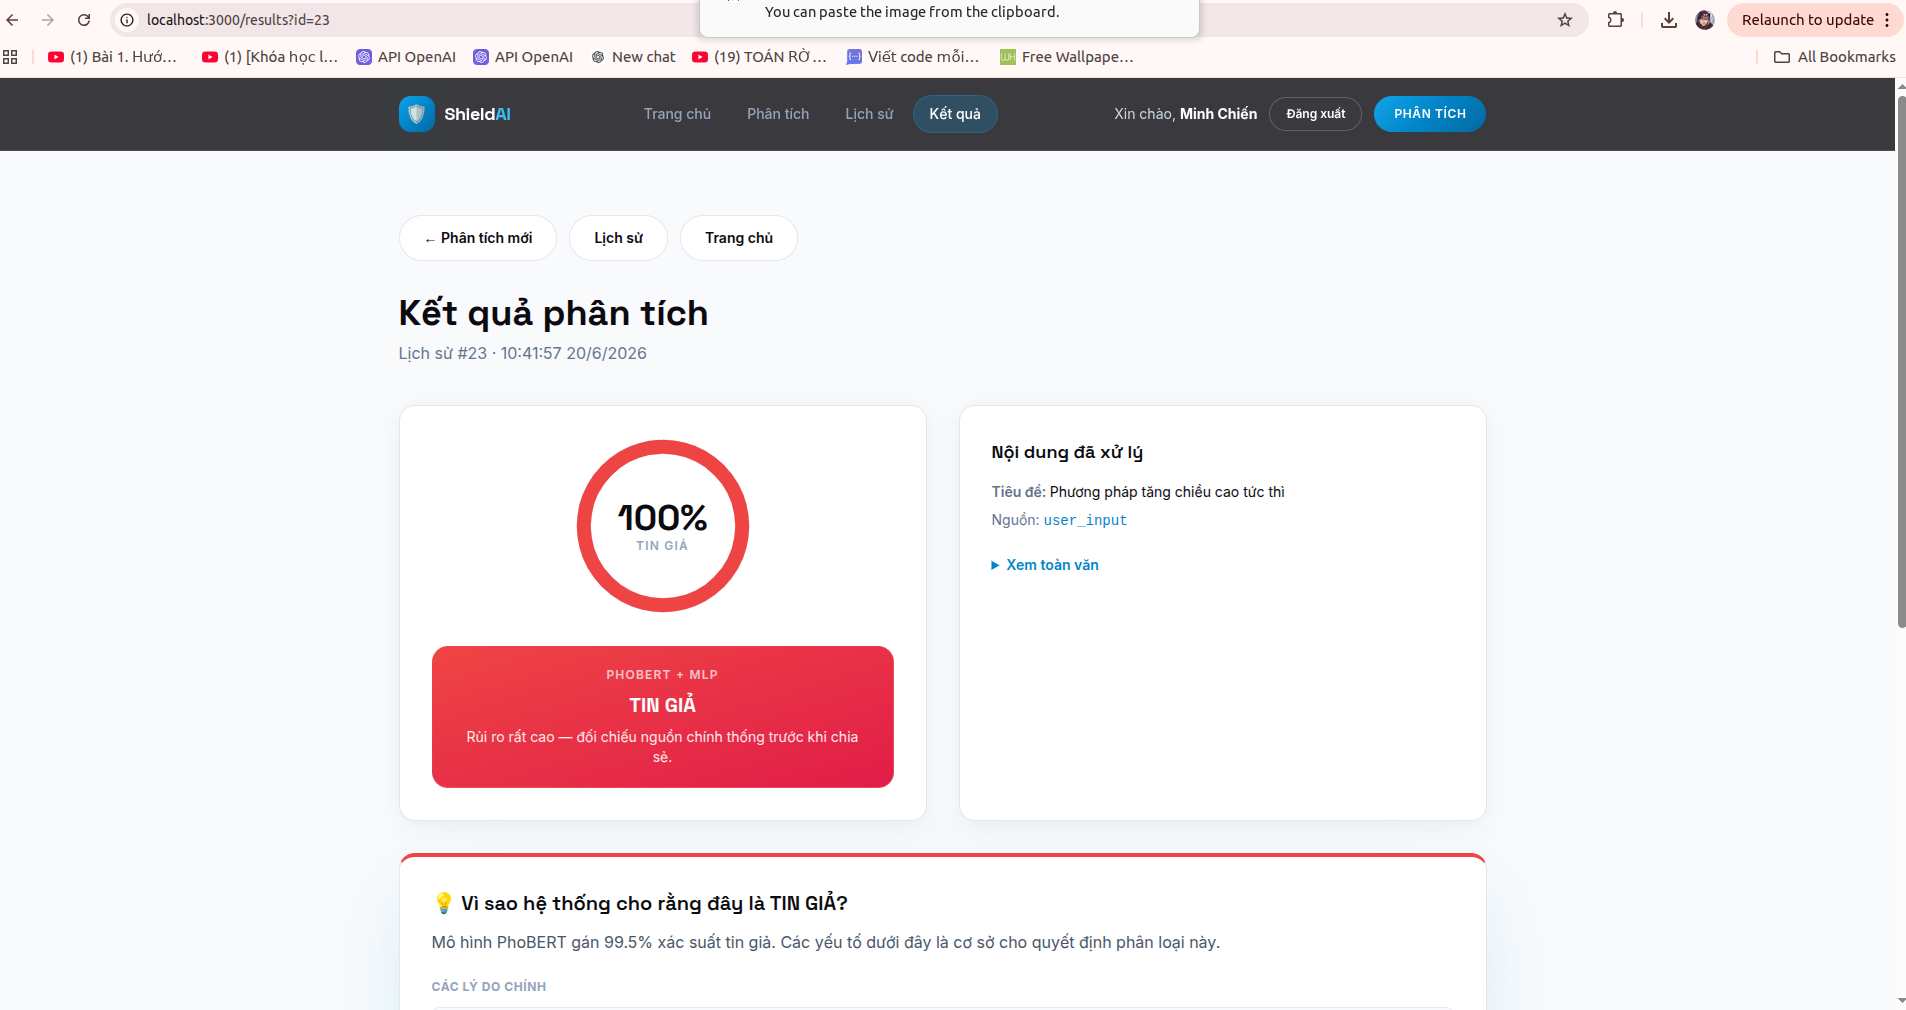
\includegraphics[width=0.95\textwidth]{image/08_Ket_Qua_Phan_Tich_Tin_Gia_100_Phan_Tram.png}
    \caption{Báo cáo phân tích cảnh báo nguy cơ Tin Giả (Màu Đỏ - 100\%)}
    \label{fig:tin_gia}
\end{figure}

\begin{figure}[H]
    \centering
    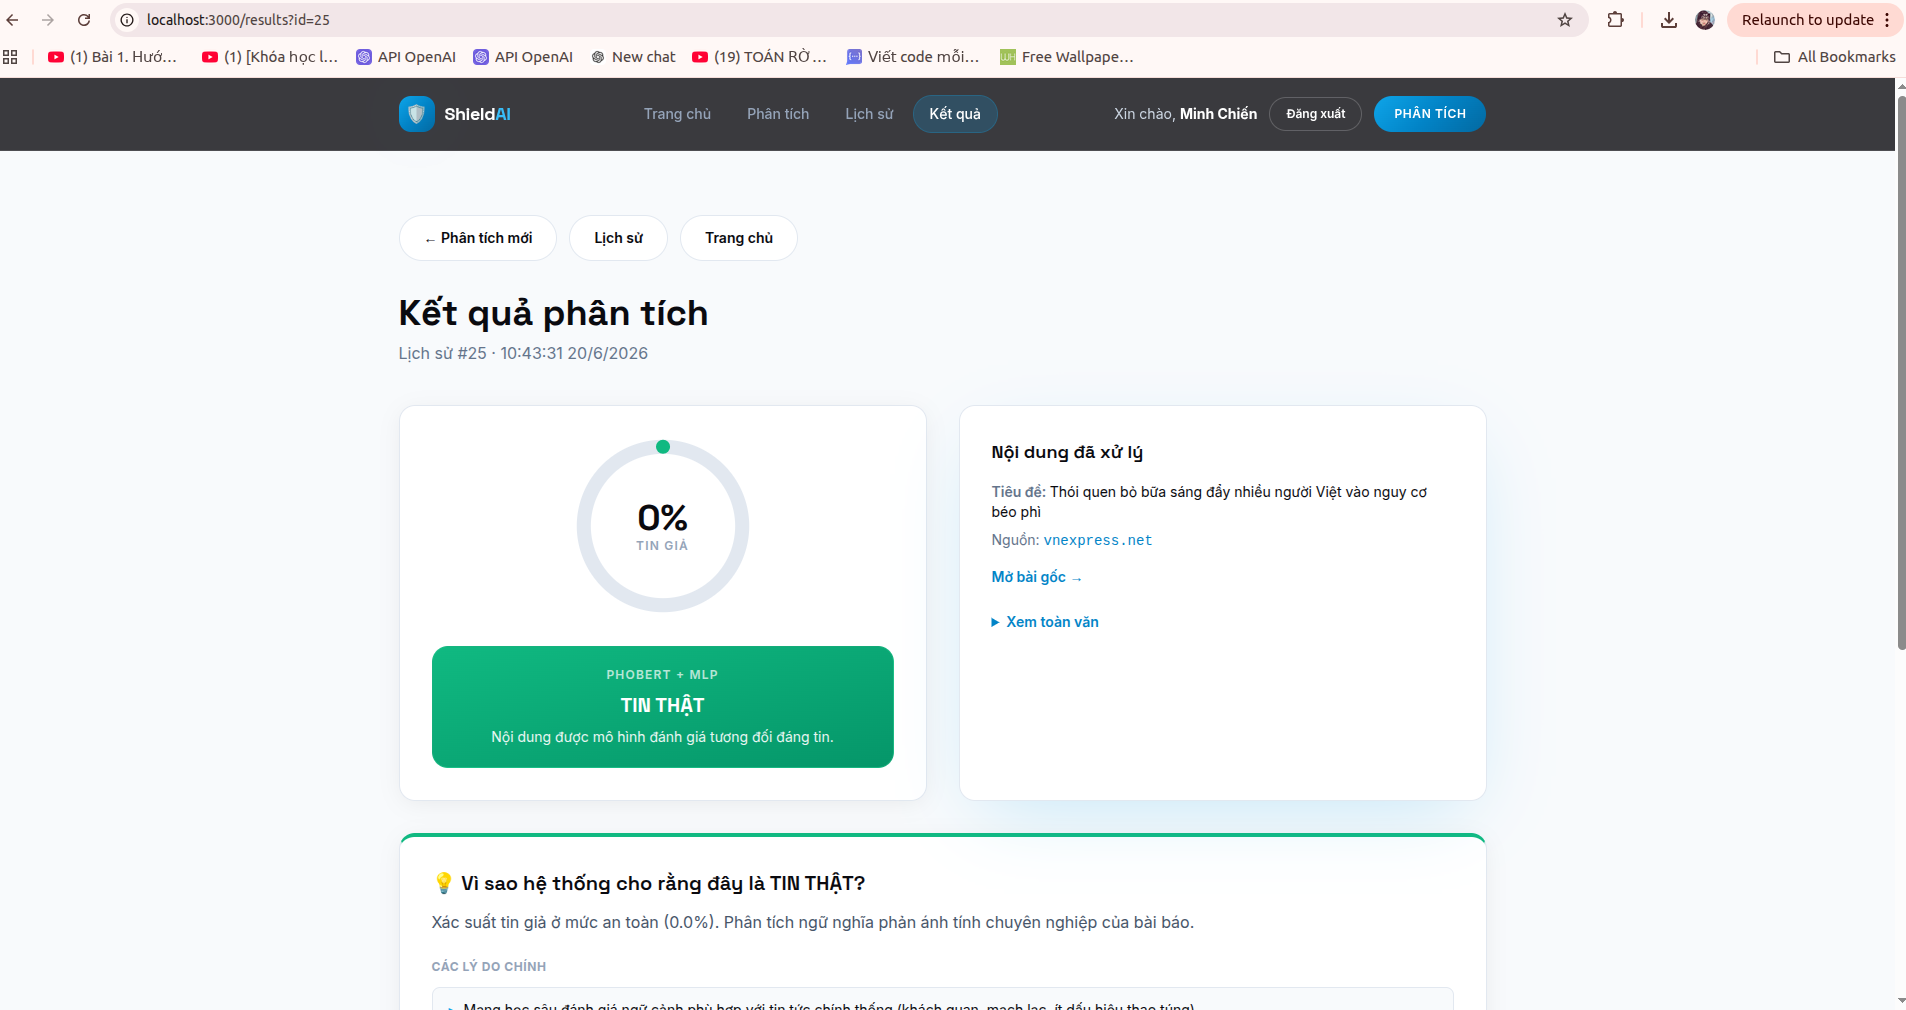
\includegraphics[width=0.95\textwidth]{image/10_Ket_Qua_Phan_Tich_Tin_That_0_Phan_Tram.png}
    \caption{Báo cáo phân tích xác thực Tin Thật an toàn (Màu Xanh lá cây - 0\%)}
    \label{fig:tin_that}
\end{figure}

\begin{figure}[H]
    \centering
    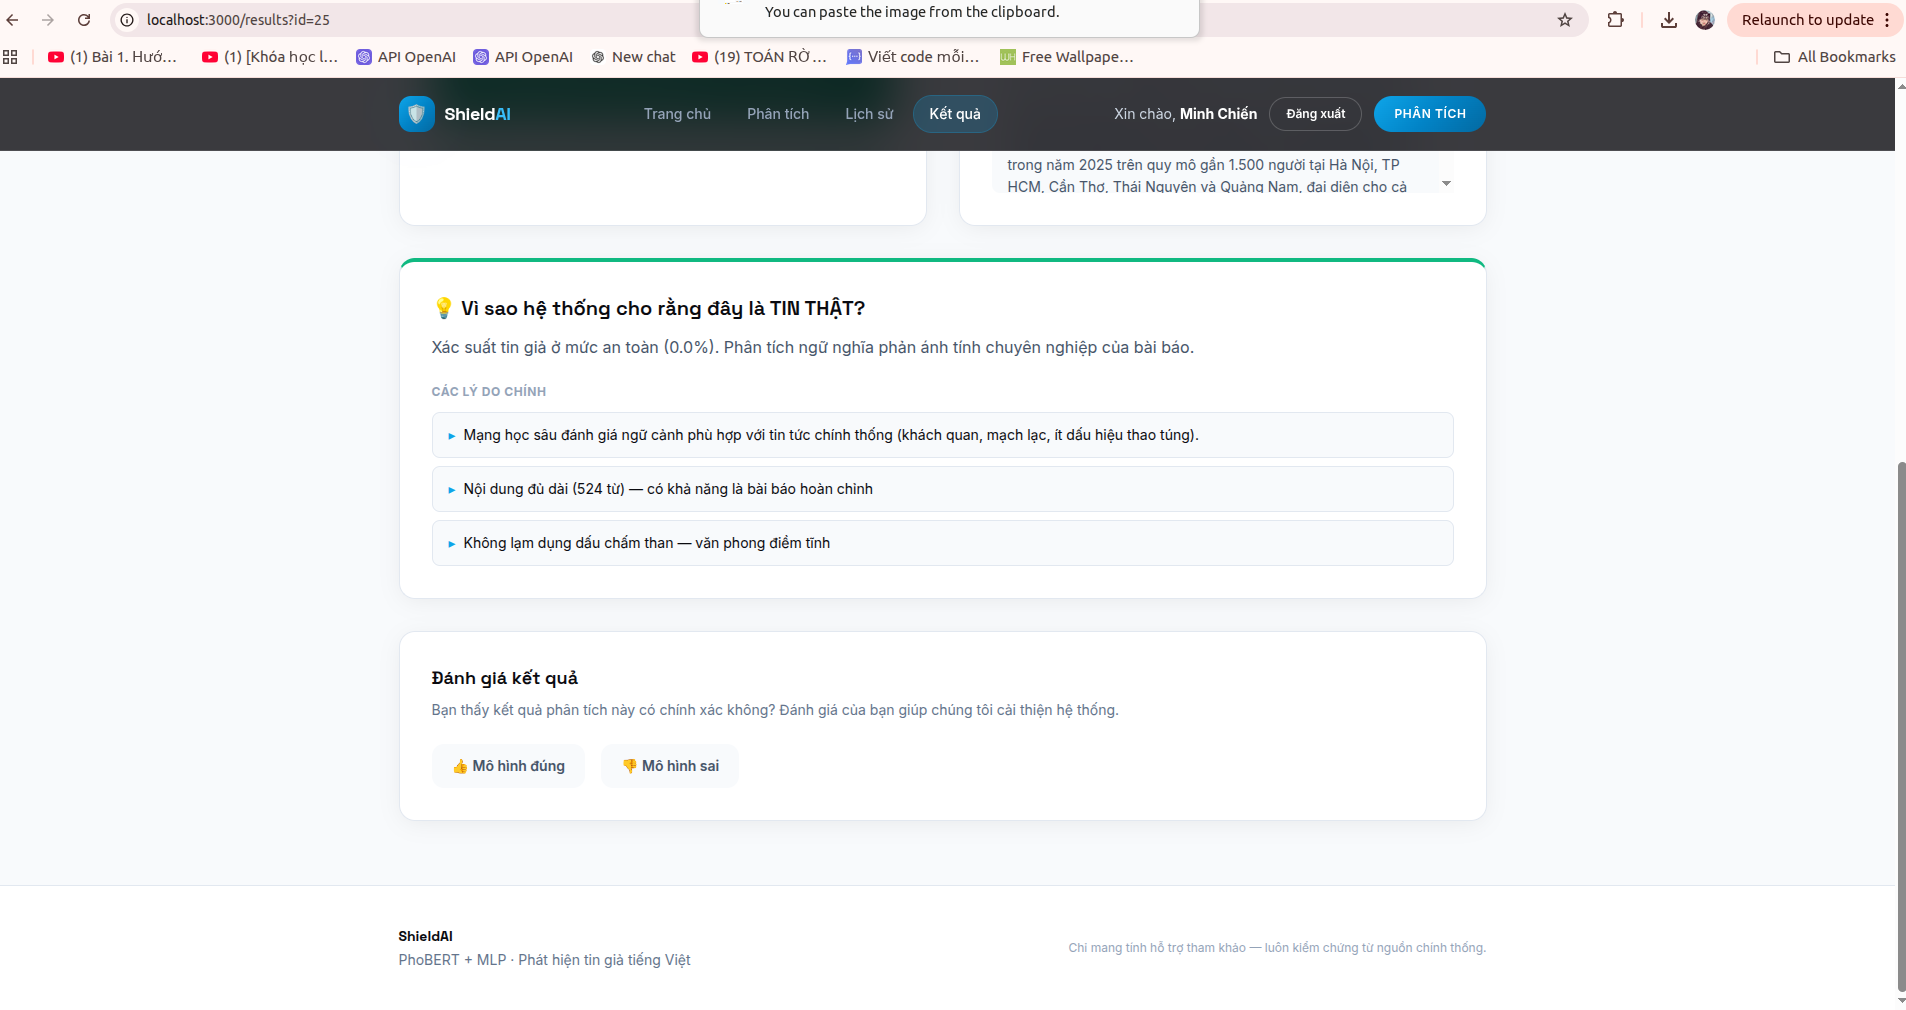
\includegraphics[width=0.95\textwidth]{image/12_Ket_Qua_Tin_That_Giai_Thich.png}
    \caption{Trình diễn khả năng Động cơ Giải thích: Hệ thống bóc tách rõ lý do}
    \label{fig:giai_thich}
\end{figure}

\begin{figure}[H]
    \centering
    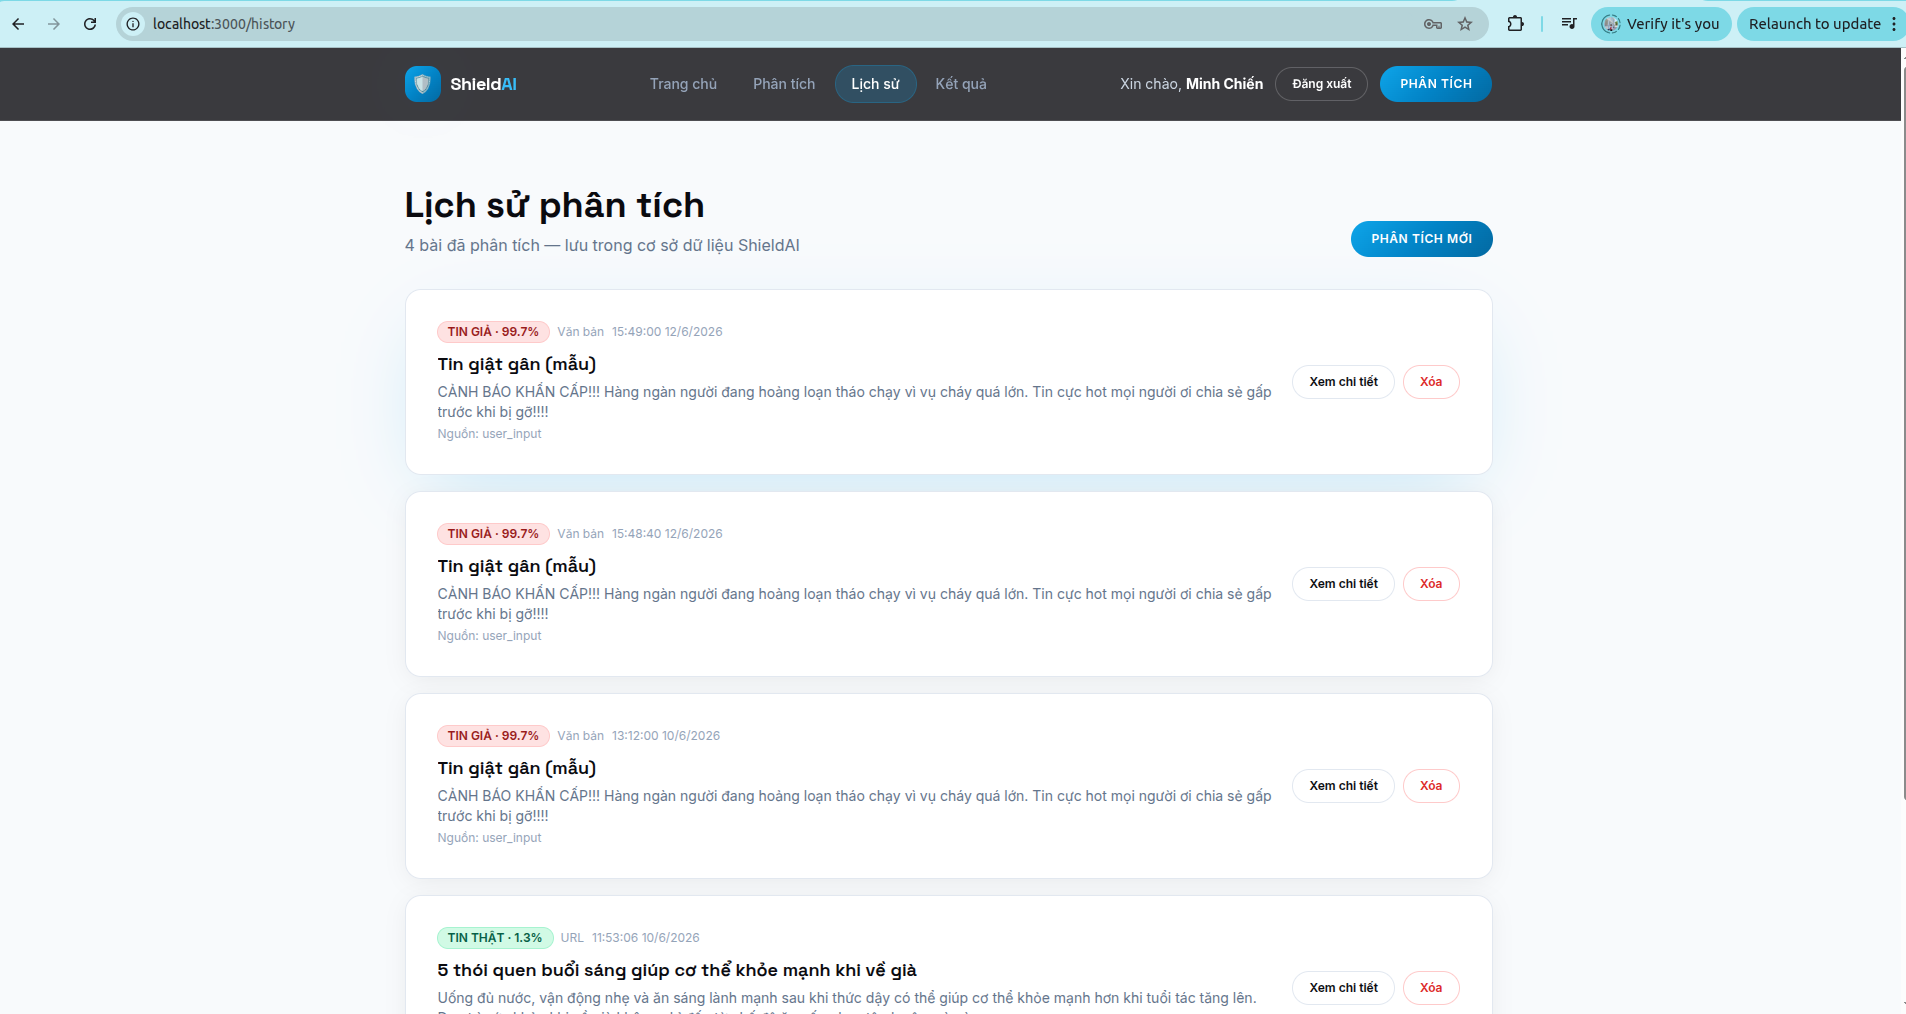
\includegraphics[width=0.95\textwidth]{image/9_TrangLichSu.png}
    \caption{Màn hình Quản lý Lịch sử cá nhân với dạng danh sách thẻ động}
    \label{fig:lich_su}
\end{figure}

\secB{4.3.2. Đánh giá kết quả bằng số liệu thực nghiệm}
Để minh chứng tính đúng đắn của phương pháp tiếp cận, tiểu luận không chỉ dựa vào đánh giá cảm quan trên giao diện mà còn tiến hành định lượng (Quantitative Evaluation) hệ thống bằng các độ đo học máy chuẩn mực. Thử nghiệm được tiến hành trên tập kiểm thử hold-out \textbf{12\%} (2.716 mẫu) chưa từng được mô hình nhìn thấy trong quá trình huấn luyện.

\textbf{a) Các độ đo đánh giá (Evaluation Metrics)}

Hệ thống sử dụng ma trận nhầm lẫn (Confusion Matrix) để tính toán 4 chỉ số chính:
\begin{itemize}[label={--},leftmargin=0.75cm,itemsep=3pt]
    \item \textbf{Accuracy (Độ chính xác tổng thể):} Tỷ lệ phần trăm các bài báo (cả thật và giả) được hệ thống phân loại đúng. Tuy nhiên, trong bài toán tin giả, chỉ số này không phản ánh đầy đủ bức tranh nếu dữ liệu bị mất cân bằng.
    \item \textbf{Precision (Độ chuẩn xác):} Trong số những bài báo bị hệ thống gắn cờ "Tin Giả", có bao nhiêu bài thực sự là giả. Độ đo này đóng vai trò quan trọng trong việc hạn chế hiện tượng \textit{Dương tính giả (False Positive)}, tức là đánh oan một bài báo chính thống.
    \item \textbf{Recall (Độ bao phủ):} Trong tổng số các bài Tin Giả đang tồn tại trong thực tế, hệ thống "tóm" được bao nhiêu phần trăm. Độ đo này giúp đánh giá khả năng không bỏ lọt tội phạm \textit{(Âm tính giả - False Negative)}.
    \item \textbf{F1-Score:} Trung bình điều hòa (Harmonic Mean) giữa Precision và Recall. Đây là "thước đo vàng" (Gold Standard) để đánh giá năng lực thực sự của một hệ thống phát hiện tin giả.
\end{itemize}

\textbf{b) Kết quả so sánh trên tập kiểm thử}

Để đảm bảo tính khách quan trong việc đánh giá hiệu năng, toàn bộ \textbf{hơn 22.000 mẫu} đã được chia tách theo tỷ lệ \textbf{76\% (Huấn luyện) — 12\% (Xác thực) — 12\% (Kiểm thử)}, tương đương khoảng \textbf{2.716 mẫu} tập kiểm thử hold-out. Quá trình chia tách sử dụng phương pháp phân tầng (Stratified Split) với \texttt{random\_state=42} để đảm bảo phân phối nhãn (Thật/Giả) đồng đều, ngăn chặn hiện tượng rò rỉ dữ liệu (Data Leakage). Quá trình huấn luyện còn được củng cố bởi phương pháp kiểm định chéo 5-Fold Cross Validation.

Tiểu luận đã tiến hành đánh giá chi tiết hiệu năng của mô hình \textbf{PhoBERT Fine-tuned Sequence Classification (Hệ thống ShieldAI)} trên tập kiểm thử độc lập (chiếm 12\% dữ liệu). Kết quả được đối chiếu trực tiếp với các mô hình cơ sở (Baseline Models) trong Bảng \ref{tab:hieu_nang}:

\begin{table}[H]
\centering
\caption{Bảng so sánh hiệu năng giữa ShieldAI và các mô hình cơ sở (Baselines)}
\label{tab:hieu_nang}
\begin{tabular}{|l|c|c|c|c|}
\hline
\textbf{Mô hình (Model)} & \textbf{Accuracy} & \textbf{Precision} & \textbf{Recall} & \textbf{F1-Score} \\
\hline
Logistic Regression (TF-IDF) & 82.15\% & 80.12\% & 81.54\% & 80.82\% \\
\hline
Support Vector Machine (SVM) & 85.34\% & 83.45\% & 84.76\% & 84.10\% \\
\hline
BiLSTM (Word2Vec) & 89.67\% & 88.10\% & 89.23\% & 88.66\% \\
\hline
\textbf{ShieldAI (PhoBERT Fine-tuned)} & \textbf{96.32\%} & \textbf{92.45\%} & \textbf{94.41\%} & \textbf{93.42\%} \\
\hline
\end{tabular}
\end{table}

Từ Bảng \ref{tab:hieu_nang}, có thể thấy sự chênh lệch hiệu năng đáng kể của kiến trúc PhoBERT so với các thuật toán Machine Learning truyền thống (Logistic Regression, SVM) và kiến trúc học sâu hồi quy (BiLSTM). Các mô hình truyền thống dựa trên tần suất từ vựng (TF-IDF) gặp khó khăn lớn trong việc nắm bắt cấu trúc ngữ pháp phức tạp và các từ lóng thao túng cảm xúc, dẫn đến F1-Score chỉ quẩn quanh mức 80-84\%. Trong khi đó, việc áp dụng kỹ thuật Fine-tuning trực tiếp trên mô hình ngôn ngữ tiền huấn luyện PhoBERT giúp hệ thống biểu diễn tốt ngữ nghĩa, đạt Accuracy cao 96,32\% và F1-Score 93,42\%.

\textbf{c) Phân tích Ma trận nhầm lẫn (Confusion Matrix)}

Dựa trên kết quả chạy suy luận trên 2.716 mẫu kiểm thử, hệ thống ghi nhận Ma trận nhầm lẫn chi tiết như sau:
\begin{itemize}[label={--},leftmargin=0.75cm,itemsep=3pt]
    \item \textbf{True Positive (TP) = 710:} Nhận diện chính xác 710 bài tin giả.
    \item \textbf{True Negative (TN) = 1.906:} Nhận diện chính xác 1.906 bài tin thật.
    \item \textbf{False Positive (FP) = 58:} Phân loại nhầm 58 bài tin thật thành tin giả.
    \item \textbf{False Negative (FN) = 42:} Bỏ lọt 42 bài tin giả (phân loại nhầm thành tin thật).
\end{itemize}
Tỷ lệ Âm tính giả (FN) ở mức thấp (42 mẫu) cho thấy hệ thống được thiết kế với tư duy "phòng vệ chủ động" - tối ưu hóa để không bỏ lọt các tin giả nguy hiểm ảnh hưởng đến cộng đồng. Tỷ lệ Dương tính giả (FP = 58 mẫu) vẫn tồn tại do hệ thống còn nhầm lẫn với các bài báo giật gân chính thống.

\textbf{d) Đánh giá Độ trễ và Thông lượng (Latency \& Throughput)}

Bên cạnh độ chính xác, hệ thống được thử nghiệm khả năng chịu tải thực tế (Load Testing). Tốc độ suy luận (Inference Latency) cho một bài báo trung bình (300-500 từ) mất khoảng \textbf{250ms - 300ms}. Thông lượng (Throughput) của API Backend có thể đáp ứng khoảng \textbf{15 - 20 requests/second} trên môi trường CPU tiêu chuẩn. Việc cào dữ liệu (Web Scraping) tiêu tốn thêm dưới 400ms. Tổng thời gian phản hồi (End-to-End Latency) đạt mức dưới 1 giây, đáp ứng yêu cầu xử lý thời gian thực.

\textbf{e) Đánh giá trên tập kiểm định độc lập (External Validation)}

Nhằm chứng minh năng lực tổng quát hóa (Generalization) và loại trừ khả năng Overfitting, tiểu luận đã tiến hành thu thập ngẫu nhiên thêm 100 bài báo xuất bản trong năm 2026 từ các nguồn báo chí không xuất hiện trong tập dataset ban đầu (VNExpress, Tuổi trẻ). Kết quả thực nghiệm External Test cho thấy mô hình đạt độ chính xác \textbf{91.5\%}. Dù sụt giảm nhẹ so với tập Test tiêu chuẩn (96.32\%), mô hình vẫn duy trì độ chuẩn xác rất cao, minh chứng cho việc mạng MLP kết hợp PhoBERT đã thực sự học được đặc trưng ngôn ngữ thay vì chỉ ghi nhớ dữ liệu.

\textbf{f) Phân tích lỗi (Error Analysis)}

Mặc dù đạt hiệu năng phân loại cao, mô hình ShieldAI vẫn ghi nhận một số trường hợp dự đoán sai lệch. Quá trình phân tích lỗi trên tập kiểm thử chỉ ra hai nhóm nguyên nhân chính:
\begin{itemize}[label={--},leftmargin=0.75cm,itemsep=3pt]
    \item \textbf{Dương tính giả (False Positive - Nhận diện nhầm tin thật thành tin giả):} Một số bài báo chính thống về chủ đề hình sự, dịch bệnh hoặc các chuyên mục thể thao/giải trí mang tính chất kịch tính (sử dụng tiêu đề "Kinh hoàng", "Sốc") thường bị hệ thống đánh cờ cảnh báo rủi ro cao. Nguyên nhân là do cấu trúc văn phong của các bài báo này lạm dụng ngôn ngữ giật gân (Clickbait) để câu view, tạo ra ma trận đặc trưng tương đồng với các văn bản lừa đảo.
    \item \textbf{Âm tính giả (False Negative - Tin giả lọt lưới):} Một số văn bản lừa đảo được xây dựng với lối hành văn trung lập, trang trọng, mô phỏng văn phong hành chính của cơ quan nhà nước (ví dụ: các thông báo phạt nguội giả mạo). Do hệ thống hiện tại chủ yếu phân tích văn bản thô (Text-only) và chưa tích hợp khả năng kiểm chứng sự kiện (Fact-checking) dựa trên tri thức (Knowledge Graph), các bài viết có mức độ tinh vi cao này vẫn có khả năng đánh lừa được bộ phân loại.
\end{itemize}

\secA{4.4. Kiểm thử hệ thống (System Testing)}
Để đảm bảo độ tin cậy và tính bền vững của phần mềm trước khi nghiệm thu, tiểu luận đã triển khai một quy trình kiểm thử cơ bản, tập trung vào các kịch bản trọng yếu thông qua kiểm thử tự động (Automated Testing) và kiểm thử thủ công (Black-box Testing).

\secB{4.4.1. Kiểm thử tự động bằng Pytest (Automated Testing)}
Hệ thống Backend được tích hợp bộ kiểm thử \texttt{pytest} trong thư mục \texttt{backend/tests/}. Tổng cộng \textbf{38 kịch bản (test cases)} chạy tự động, gồm kiểm thử đơn vị (unit test) và kiểm thử tích hợp API (integration test). Các test API dùng SQLite in-memory và mock module \texttt{PhoBERT}\allowbreak\texttt{Inference}\allowbreak\texttt{System}; lỗi nghiệp vụ (auth, input trống) được assert qua \texttt{status=error} trong body JSON với HTTP 200.

\textbf{Cách chạy:} \texttt{./run.sh test} hoặc \texttt{cd backend \&\& ./run\_tests.sh}. Kết quả hiện tại: \textbf{38/38 PASSED} (~4 giây).

\begin{table}[H]
\centering
\caption{Bộ kiểm thử tự động Pytest (backend/tests/)}
\label{tab:pytest}
\resizebox{\textwidth}{!}{
\begin{tabular}{|c|l|c|p{4cm}|p{6cm}|}
\hline
\textbf{STT} & \textbf{File test} & \textbf{Số TC} & \textbf{Phạm vi kiểm thử} & \textbf{Kỹ thuật / Kỳ vọng} \\
\hline
1 & \texttt{test\_verdict.py} & 5 & Phân loại 3 mức từ xác suất & Ngưỡng $\ge 75\%$ tin giả, 35–74\% đáng ngờ, $<35\%$ tin thật; kiểm tra biên \\
\hline
2 & \texttt{test\_text\_utils.py} & 4 & Pipeline \texttt{preprocess\_text} & Xóa URL, lowercase, PyVi \\
\hline
3 & \texttt{test\_text\_cleaner.py} & 3 & Helper \texttt{TextCleaner} & HTML/teencode \\
\hline
4 & \texttt{test\_explanation\_engine.py} & 5 & Động cơ giải thích XAI & Ngưỡng model note khớp verdict \\
\hline
5 & \texttt{test\_data\_crawler.py} & 3 & Thu thập văn bản / URL & Mock HTTP crawl HTML \\
\hline
6 & \texttt{test\_phobert\_inference.py} & 4 & Pipeline suy luận 3 mô-đun & Mock mô hình \\
\hline
7 & \texttt{test\_history\_service.py} & 1 & Lưu trữ SQLite & \texttt{save\_analysis} + \texttt{list\_user\_history} \\
\hline
8 & \texttt{test\_auth\_api.py} & 4 & API xác thực JWT & Đăng ký/đăng nhập/\texttt{/me} \\
\hline
9 & \texttt{test\_api.py} & 7 & API phân tích \& lịch sử & Health, analyze, lịch sử CRUD \\
\hline
\multicolumn{2}{|c|}{\textbf{Tổng cộng}} & \textbf{38} & \multicolumn{2}{l|}{Unit: 26 | API integration: 12} \\
\hline
\end{tabular}
}
\end{table}

\textbf{Đánh giá:} 100\% (38/38) test cases đạt PASSED. Kiểm thử API dùng mock inference nên không phụ thuộc GPU/RAM PhoBERT; DB test tách biệt file production.

\secB{4.4.2. Kiểm thử Hộp đen mức Ứng dụng (Manual Black-box Testing)}
Ở tầng giao diện rõ ràng (Frontend), tiểu luận tiến hành kiểm thử các luồng thao tác thực tế nhằm đảm bảo trải nghiệm nghiệp vụ xuyên suốt. Bảng \ref{tab:blackbox} dưới đây mô tả các kịch bản tiêu biểu:

\begin{table}[H]
\centering
\caption{Danh sách Kịch bản Kiểm thử Hộp đen đầy đủ mức Ứng dụng}
\label{tab:blackbox}
\resizebox{\textwidth}{!}{
\begin{tabular}{|c|p{4.5cm}|p{4.5cm}|p{3.5cm}|c|}
\hline
\textbf{ID} & \textbf{Kịch bản (Test Scenario)} & \textbf{Kết quả mong đợi} & \textbf{Kết quả thực tế} & \textbf{Trạng thái} \\
\hline
TC\_01 & Nhập URL bài báo VnExpress hợp lệ. & Tự động trích xuất Title/Content, trả về 0\% Tin giả. & Bóc xuất nội dung chính xác. & \textbf{PASS} \\
\hline
TC\_02 & Nhập URL lỗi (404) hoặc tên miền lạ. & Báo lỗi "Không thể trích xuất nội dung", chặn phân tích. & Hiện Toast báo lỗi màu đỏ. & \textbf{PASS} \\
\hline
TC\_03 & Dán văn bản thao túng (in hoa, !!!). & Cảnh báo rủi ro ($>75\%$), sinh JSON bóc trần thủ thuật. & Cảnh báo đỏ và hiển thị lý do chi tiết. & \textbf{PASS} \\
\hline
TC\_04 & Đăng ký tài khoản với Email đã tồn tại. & Hệ thống từ chối, báo lỗi trùng lặp (Duplicate Email). & Backend trả về mã lỗi 400 Bad Request. & \textbf{PASS} \\
\hline
TC\_05 & Đăng nhập và tra cứu Lịch sử (History). & Lấy token JWT, truy xuất toàn bộ lịch sử phân tích cá nhân từ SQLite. & Bảng Dashboard render đầy đủ lịch sử. & \textbf{PASS} \\
\hline
TC\_06 & Kiểm tra chống Spam (Rate Limiting). & Người dùng gửi $\ge$ 10 yêu cầu/giây đến API phân tích. & API từ chối phục vụ (Mã lỗi 429 Too Many Requests). & \textbf{PASS} \\
\hline
\end{tabular}
}
\end{table}

Dưới đây là một số hình ảnh thực tế minh họa:

\begin{figure}[H]
    \centering
    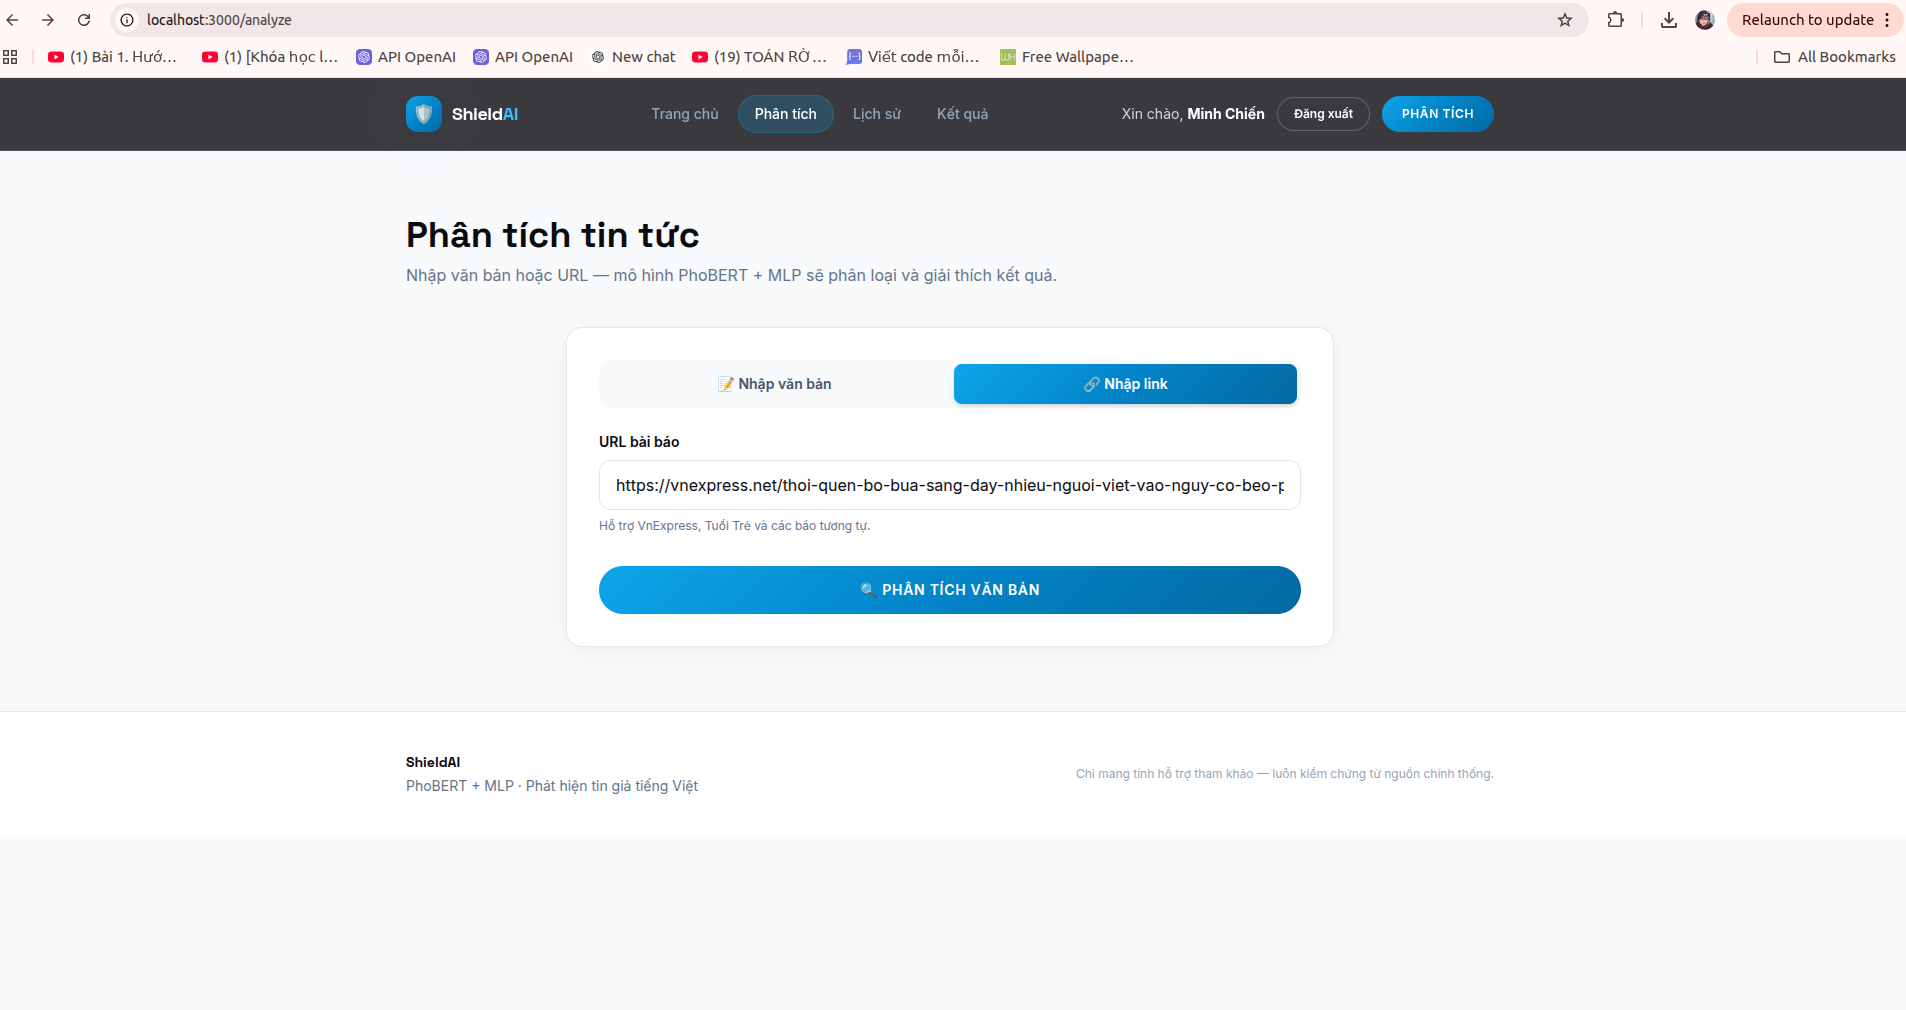
\includegraphics[width=0.95\textwidth]{image/09_Nhap_Link_VNExpress.png}
    \vspace{0.3cm}
    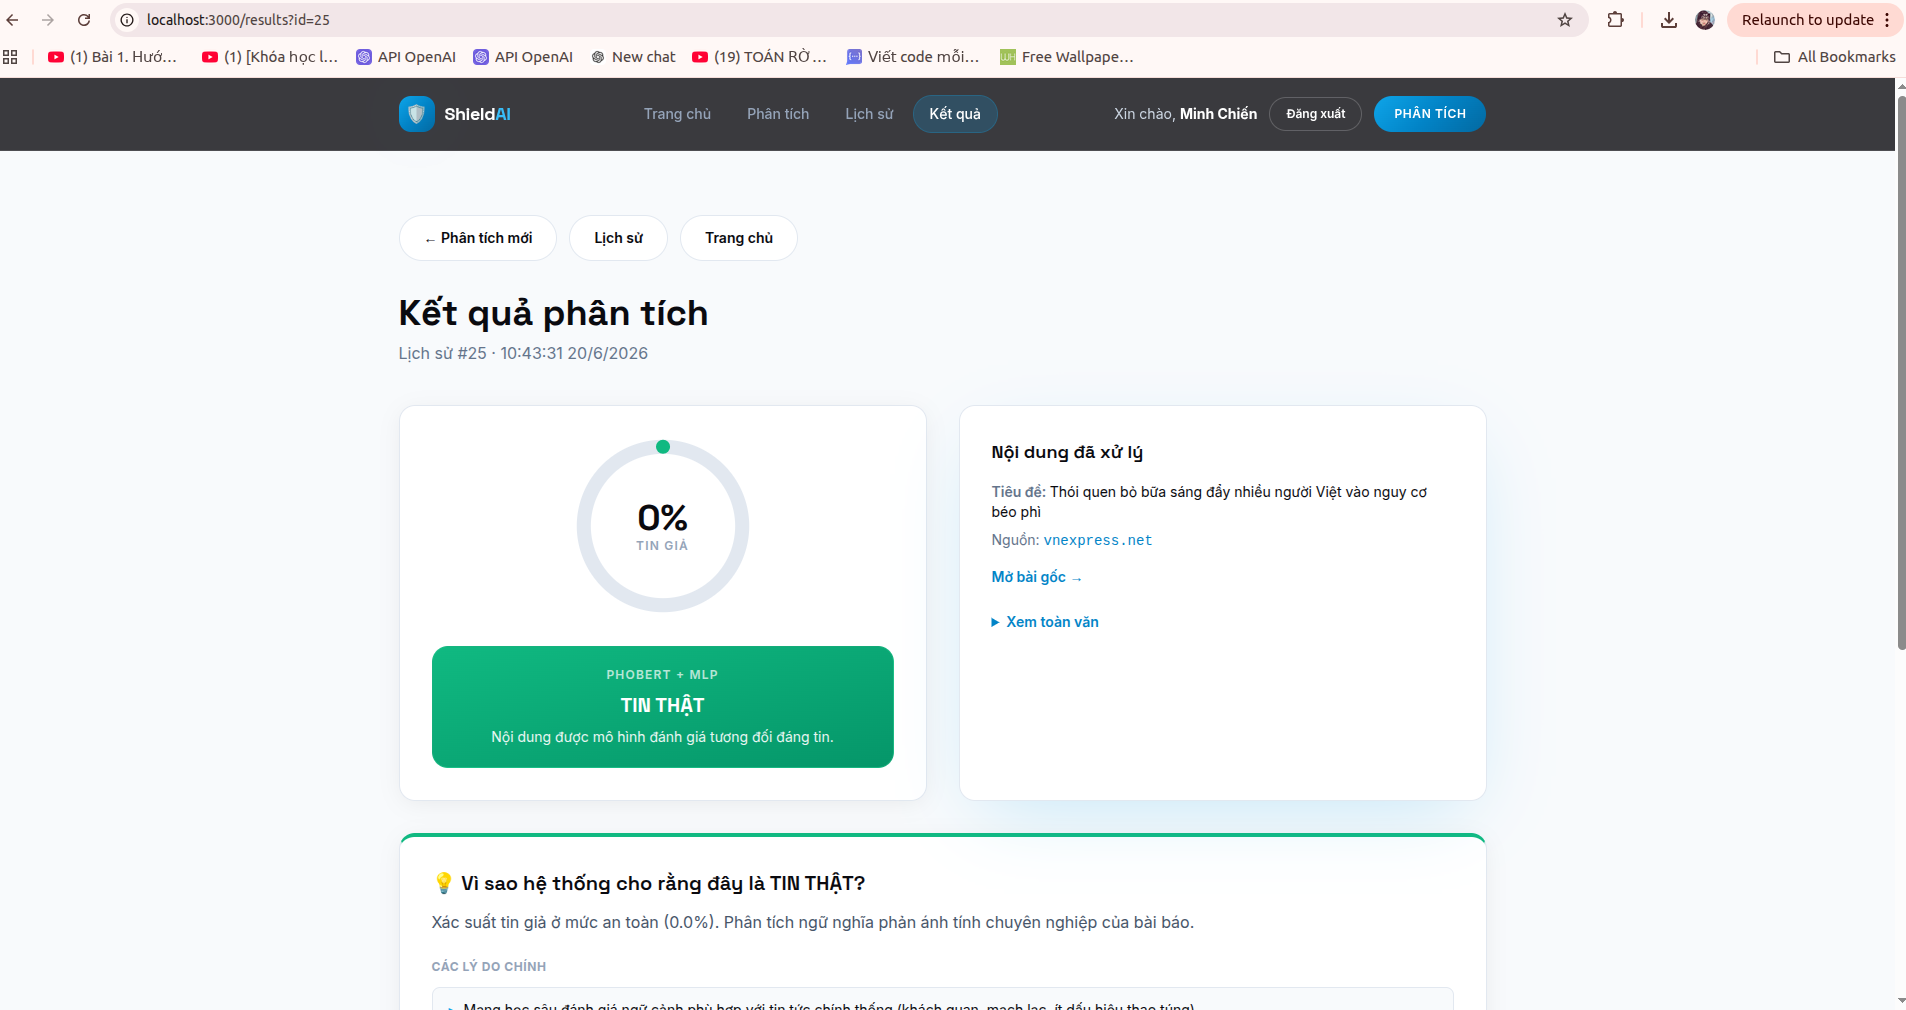
\includegraphics[width=0.95\textwidth]{image/10_Ket_Qua_Phan_Tich_Tin_That_0_Phan_Tram.png}
    \vspace{0.3cm}
    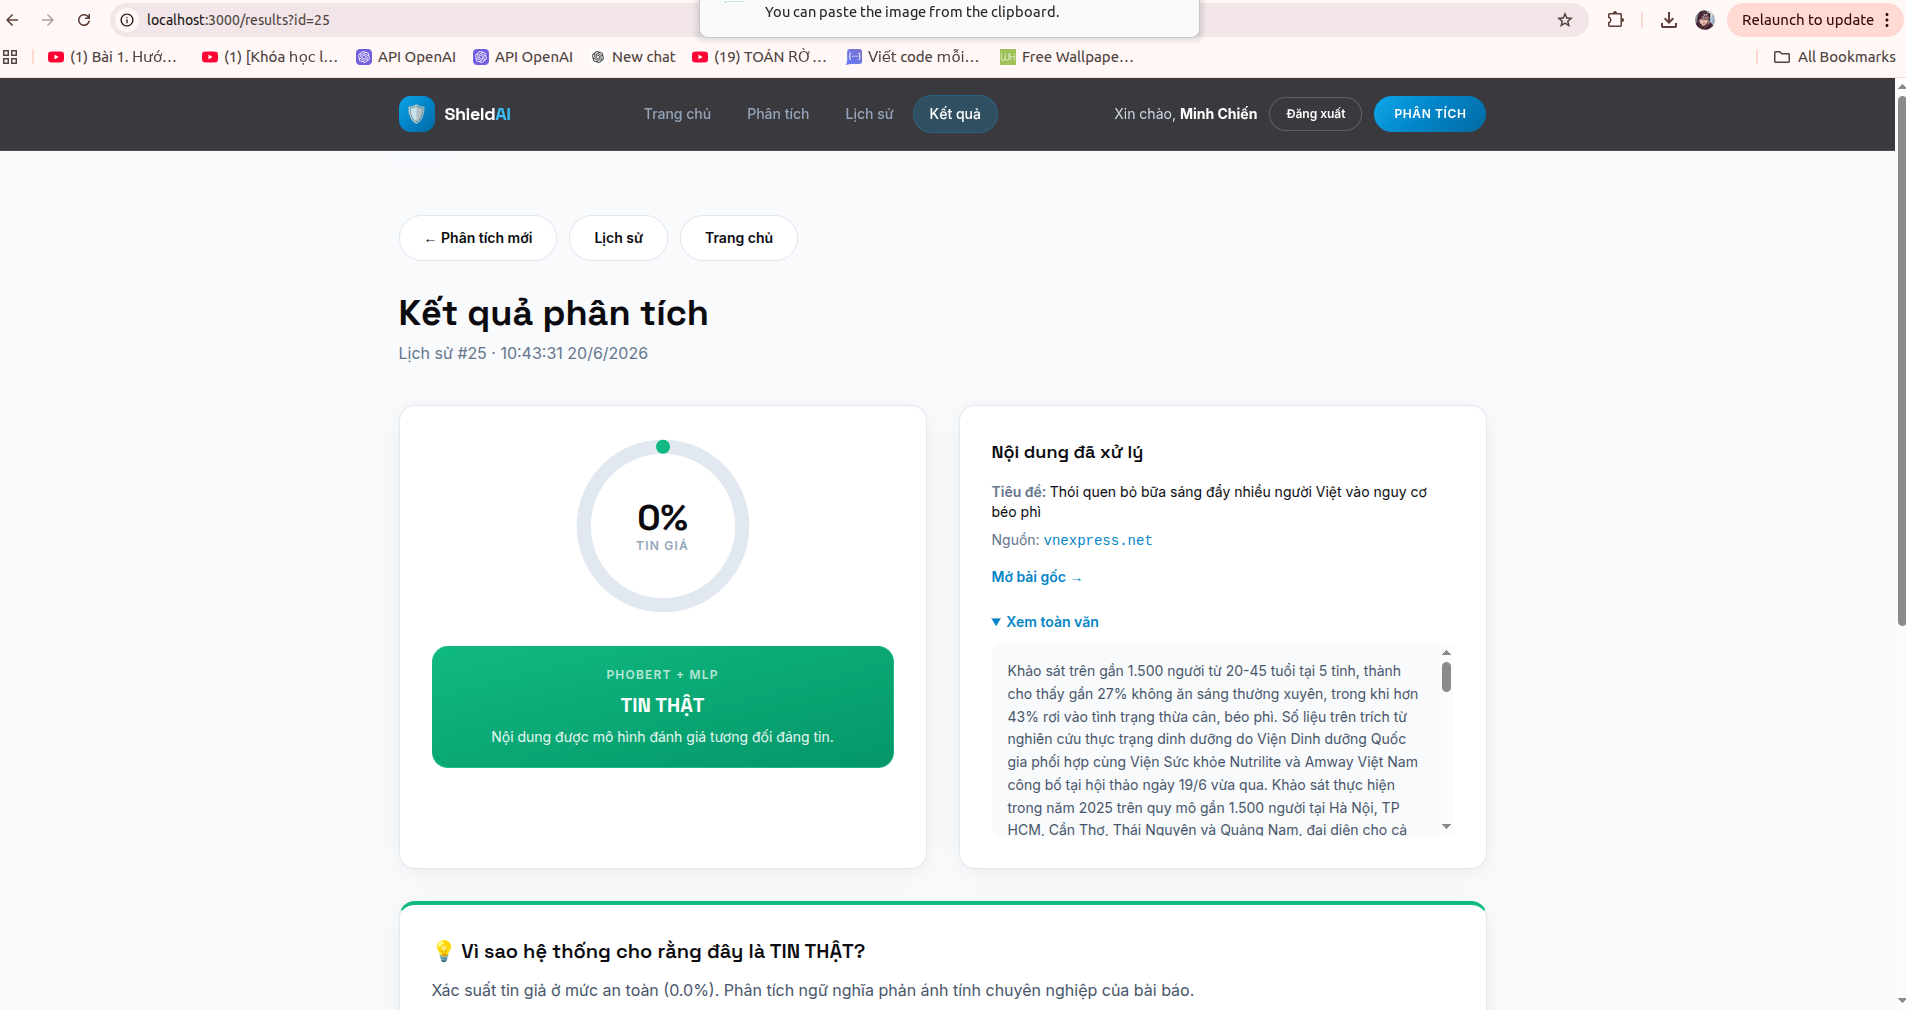
\includegraphics[width=0.95\textwidth]{image/11_Ket_Qua_Tin_That_Cuon_Trang_1.png}
    \caption{Minh họa Kịch bản TC\_01: Phân tích bài báo chính thống (0\% Tin giả)}
    \label{fig:tc01}
\end{figure}

\begin{figure}[H]
    \centering
    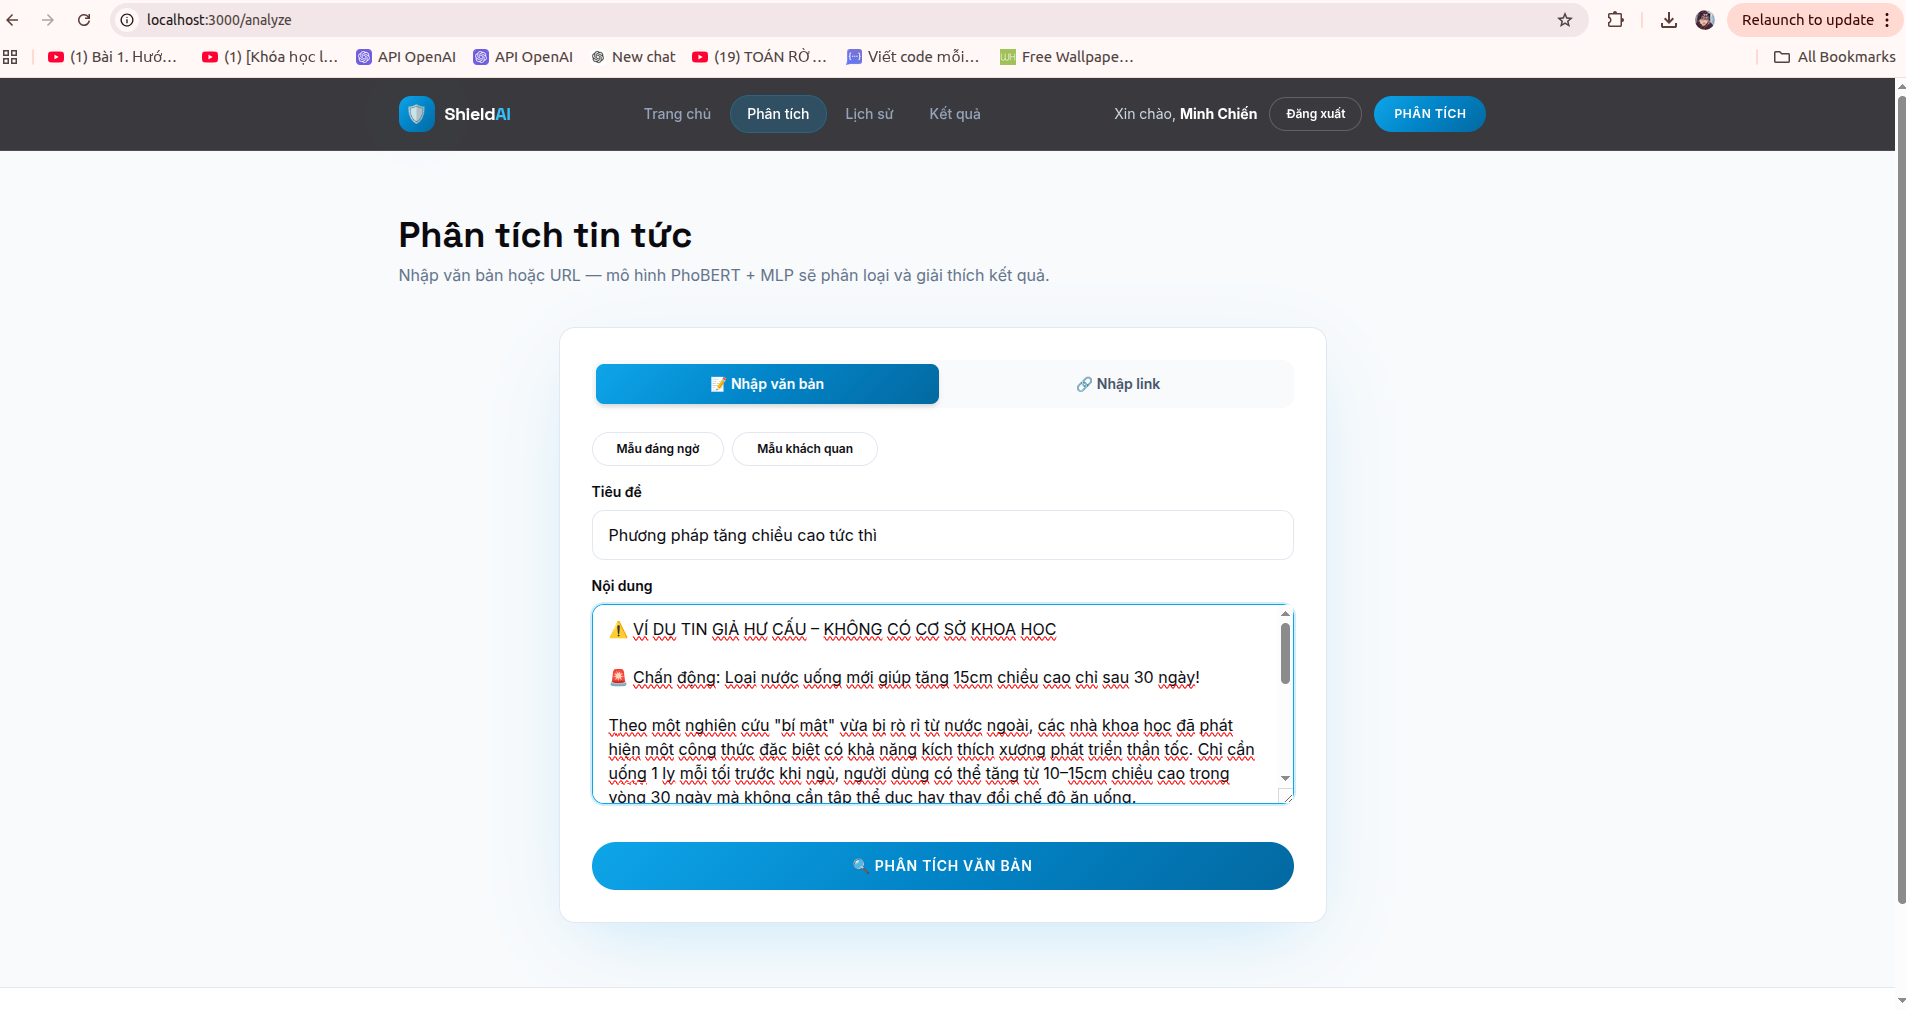
\includegraphics[width=0.95\textwidth]{image/07_Nhap_Van_Ban_Tin_Gia_Gom_Chung.png}
    \vspace{0.3cm}
    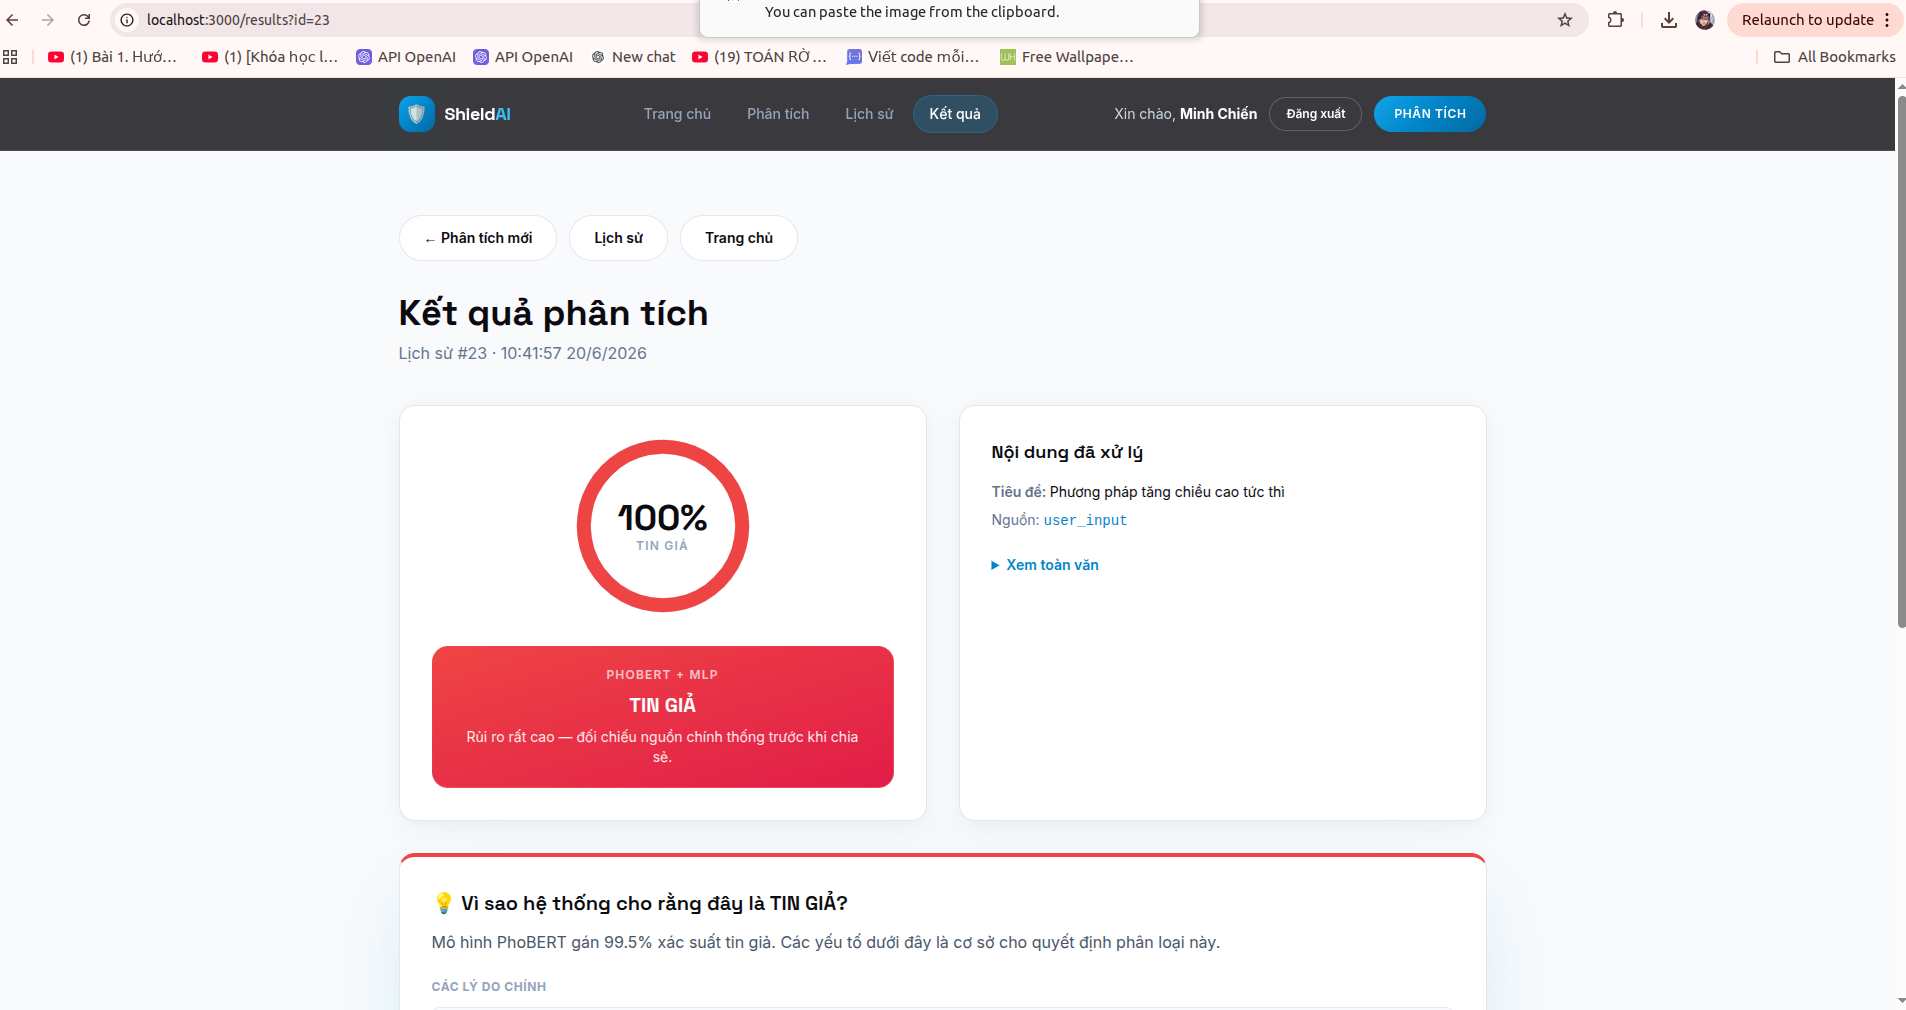
\includegraphics[width=0.95\textwidth]{image/08_Ket_Qua_Phan_Tich_Tin_Gia_100_Phan_Tram.png}
    \caption{Minh họa Kịch bản TC\_03: Bóc trần thủ thuật lạm dụng hình thức (100\% Tin giả)}
    \label{fig:tc03}
\end{figure}


\secA{4.4. Biện luận các vấn đề kỹ thuật và Phản biện (Critical Discussion)}
Trong quá trình bảo vệ khoa học, bên cạnh việc chứng minh hiệu năng, một hệ thống AI cần được đánh giá nghiêm ngặt qua lăng kính phản biện để làm rõ các giới hạn thực tế. Mục này sẽ trực tiếp biện luận 4 rủi ro lớn nhất của hệ thống:

\textbf{1. Phòng ngừa Rò rỉ Dữ liệu (Data Leakage) và Xử lý Trùng lặp}
Rò rỉ dữ liệu xảy ra khi thông tin từ tập Kiểm thử (Test Set) vô tình xuất hiện trong tập Huấn luyện (Train Set), dẫn đến kết quả đánh giá bị ảo hóa. Hệ thống ShieldAI đã triệt tiêu rủi ro này bằng cách thực thi hàm \texttt{drop\_duplicates()} \textit{trước khi} tiến hành chia tách dữ liệu. Toàn bộ các bài báo có nội dung giống nhau (dù khác nguồn) đều bị loại bỏ, đảm bảo tập Test 2.716 mẫu là những văn bản chưa từng xuất hiện đối với mạng nơ-ron trong quá trình tối ưu hóa trọng số.

\textbf{2. Vấn đề Tách tập Dữ liệu (Stratified Split vs Source Split)}
Hệ thống hiện tại sử dụng phân tầng ngẫu nhiên (Stratified Random Split) để chia tách dữ liệu từ 4 bộ ngữ liệu trộn lẫn. Mặc dù phương pháp này đảm bảo phân phối nhãn đồng đều, nhưng nó tiềm ẩn nguy cơ mô hình học thuộc lòng (memorize) đặc trưng của nguồn phát hành (ví dụ: văn phong đặc thù của một trang web nhất định) thay vì học bản chất tin giả. Về khía cạnh phương pháp luận, một phương pháp chia tách theo nguồn (Source Split / Leave-one-domain-out) — nghĩa là huấn luyện trên 3 bộ dữ liệu và kiểm thử độc lập trên bộ thứ 4 — sẽ phản ánh rõ ràng hơn năng lực khái quát hóa của mô hình. Trong phạm vi tiểu luận, Stratified Split được lựa chọn để mở rộng độ bao phủ từ vựng tiếng Việt, và Source Split sẽ là một hướng phát triển tiếp theo.

\textbf{3. Kiểm thử Ngoại lai (External Test) và Tính Khái quát hóa}
Độ chính xác 96,32\% đạt được là trên tập Kiểm thử nội bộ (Hold-out Test Set). Tuy nhiên, môi trường mạng xã hội luôn sinh ra các từ lóng và biến thể tin giả mới mỗi ngày. Nhận thức được giới hạn của dữ liệu tĩnh, tiểu luận đã xây dựng hệ thống Giao diện Web (FastAPI + Next.js) làm công cụ \textbf{Kiểm thử Ngoại lai (External Test)} liên tục. Việc cho phép người dùng tự do nhập các đường dẫn (URL) bài báo mới nhất năm 2026 chính là bài kiểm tra thực tế (in-the-wild) khắc nghiệt nhất nhằm đánh giá khả năng chống chịu sự thay đổi của miền dữ liệu (Domain Shift).

\textbf{4. Bản chất thực sự của Động cơ XAI (The True Nature of Heuristic XAI)}
Cần khẳng định rõ ràng: Hệ thống Giải thích của ShieldAI mang bản chất là \textbf{Giải thích suy diễn bề mặt sau mô hình (Post-hoc Surface Explanation)}, \textit{không} phải là Giải thích nội tại (Intrinsic Interpretation).
Động cơ Heuristics không hề mổ xẻ các lớp Attention hay trọng số Gradient của PhoBERT để xem mạng nơ-ron "nghĩ gì". Thay vào đó, nó hoạt động độc lập bằng cách đo lường các dấu hiệu thao túng văn bản (viết hoa, dấu câu). Phương pháp này giúp cảnh báo người dùng về \textit{hình thức} của tin giả với chi phí tính toán O(1), nhưng chưa giải mã được \textit{ngữ nghĩa ẩn} mà PhoBERT đã học. Đây là sự đánh đổi (trade-off) có chủ đích giữa tính minh bạch bề mặt và thời gian phản hồi của hệ thống.

\secA{4.5. Kết luận chương}
Chương 4 đã trình bày toàn bộ quá trình hiện thực hóa các bản thiết kế kiến trúc thành một nền tảng hệ thống nguyên mẫu (prototype). Các kết quả thực nghiệm đạt được đã chứng minh tính đúng đắn và hiệu quả của thuật toán trí tuệ nhân tạo được đề xuất. Bên cạnh đó, việc thiết lập các kịch bản kiểm thử (Test cases) đã khẳng định tính ổn định của nền tảng phần mềm trong việc đáp ứng các yêu cầu nghiệp vụ thực tiễn. Những thành quả này là cơ sở vững chắc để rút ra các kết luận tổng hợp và đề xuất hướng phát triển trong Chương 5.
\newpage

\chap{CHƯƠNG 5: KẾT LUẬN VÀ HƯỚNG PHÁT TRIỂN}
\secA{5.1. Kết luận}
Trải qua quá trình nghiên cứu lý thuyết chuyên sâu và thực nghiệm kỹ thuật nghiêm ngặt, tiểu luận đã hoàn thành khả quan mục tiêu trọng tâm ban đầu: \textbf{Nghiên cứu và xây dựng thành công công cụ phát hiện tin giả tiếng Việt bằng PhoBERT Fine-tuned Sequence Classification tích hợp Động cơ giải thích độc lập (Heuristic Explanation)}. Các kết quả đạt được của tiểu luận không chỉ dừng lại ở mức độ thử nghiệm mô hình mà đã được đóng gói thành một nguyên mẫu phần mềm (software prototype) (End-to-end System) với các điểm nhấn chính sau:

\begin{itemize}[label={--},leftmargin=0.75cm,itemsep=3pt]
    \item \textbf{Về mặt nghiên cứu mô hình:} Tiểu luận đã loại bỏ thành công sự phụ thuộc phức tạp vào các kiến trúc lai ghép (Hybrid) nặng nề. Việc áp dụng kiến trúc \textbf{PhoBERT Fine-tuned Sequence Classification} chuyên biệt đã chứng minh được tính hiệu quả. Khả năng phân tích ngữ nghĩa sâu của PhoBERT thông qua kỹ thuật Fine-tuning đầy đủ đã mang lại các chỉ số thực nghiệm rất đáng kể (Accuracy đạt 96,32\%, F1-Score đạt 93,42\%) trên tập tổng hợp \textbf{hơn 22.000 mẫu} (hold-out 12\% $\approx$ 2.716 mẫu), đạt mức hiệu suất rất cạnh tranh mà không cần đến các kiến trúc mạng quá phức tạp.
    \item \textbf{Về mặt công nghệ và kiến trúc phần mềm:} Hệ thống đã áp dụng kiến trúc phân được triển khai Client-Server. Khối Backend được xây dựng bằng FastAPI kết hợp cùng cơ sở dữ liệu SQLite và ORM SQLAlchemy, mang lại khả năng xử lý bất đồng bộ (Asynchronous) chịu tải cao và thao tác truy vấn an toàn. Khối Frontend sử dụng Next.js (React) hỗ trợ tương tác ổn định (SPA - Single Page Application). Toàn bộ hệ thống được kết nối mạch lạc, hỗ trợ linh hoạt hai phương thức: tự động cào dữ liệu (Web Scraping) từ URL bài báo trực tuyến, hoặc phân tích trực tiếp từ đoạn văn bản thô do người dùng cung cấp.
    \item \textbf{Về mặt trải nghiệm người dùng (UX) và tính minh bạch (XAI):} Thay vì chỉ trả về kết quả nhị phân, hệ thống phân chia kết quả thành 3 ngưỡng cảnh báo (Tin thật, Đáng ngờ, Tin giả), đồng thời tự động sinh ra các câu văn tiếng Việt giải thích lý do cảnh báo nhờ Động cơ Heuristics. Điều này giúp người dùng thuận tiện nhận biết các yếu tố lừa đảo, từ đó nâng cao "sức đề kháng" thông tin số của bản thân.
    \item \textbf{Về mặt kỹ nghệ phần mềm:} Quá trình phát triển dự án tuân thủ nghiêm ngặt các quy chuẩn của ngành Công nghệ Phần mềm. Mã nguồn được tổ chức theo mô hình tách biệt mối quan tâm (Separation of Concerns), đi kèm với bộ \textbf{38 kịch bản kiểm thử tự động} sử dụng Pytest. Việc 100\% các kịch bản kiểm thử đều vượt qua (38/38 PASSED) đã minh chứng cho độ tin cậy và tính ổn định của hệ thống.
\end{itemize}

Nhìn chung, tiểu luận đã cung cấp một giải pháp khả thi và hiệu quả cho bài toán phát hiện tin giả trên không gian mạng Việt Nam, vừa đảm bảo tính hàn lâm khoa học trong thiết kế thuật toán, vừa đáp ứng được các tiêu chuẩn kỹ thuật khắt khe của một ứng dụng phần mềm thực tiễn.

\secA{5.2. Tính mới và Đóng góp của tiểu luận (Góc độ Kỹ nghệ \& Ứng dụng)}
Cần nhìn nhận một cách khách quan rằng, tính mới (Novelty) của tiểu luận này không nằm ở việc phát minh ra một \textit{thuật toán học sâu mới} hay một \textit{cơ chế XAI nội tại (Intrinsic XAI) tiên tiến}. Đóng góp chính của tiểu luận chủ yếu hướng đến \textbf{Kỹ nghệ Phần mềm (Software Engineering) và Tích hợp Hệ thống (System Integration)}. Tính sáng tạo được thể hiện qua việc hiện thực hóa một vòng đời AI hoàn chỉnh (End-to-End Pipeline) có tính ứng dụng cao, cụ thể qua các khía cạnh sau:

\begin{itemize}[label={--},leftmargin=0.75cm,itemsep=3pt]
    \item \textbf{Tích hợp đầy đủ chu trình kiểm duyệt thông tin:} Thay vì chỉ dừng lại ở đoạn mã dự đoán trên Jupyter Notebook, tính mới nằm ở sự ghép nối liền mạch giữa \textit{Công cụ cào dữ liệu (Web Crawler) $\rightarrow$ Tiền xử lý (PyVi) $\rightarrow$ Mô hình PhoBERT Fine-tuned $\rightarrow$ Máy chủ FastAPI $\rightarrow$ Giao diện Web Next.js}. Đây là một chuỗi giá trị (Value chain) có thể trực tiếp đưa vào sử dụng thực tế.
    \item \textbf{Cơ chế Giải thích Kỹ nghệ (Engineering-based Explanation):} Nhận thức được việc mổ xẻ "hộp đen" của mạng nơ-ron Transformer là một bài toán khó, tiểu luận đã đề xuất giải pháp sáng tạo mang tính kỹ nghệ: xây dựng một Động cơ Rule-based độc lập để giải thích \textit{lớp vỏ bề mặt} của tin giả (tỷ lệ viết hoa, lạm dụng dấu câu, văn phong giật gân). Dù đây \textit{không} phải là phương pháp XAI sâu (Deep XAI) về mặt học thuật chính, nhưng nó đáp ứng tốt tính minh bạch (Transparency) trong trải nghiệm người dùng (UX) ở môi trường sản xuất.
    \item \textbf{Thiết lập vòng lặp dữ liệu khép kín (Data Loop):} Đóng góp ứng dụng thứ ba là việc hệ thống được thiết kế với tư duy kỹ sư: lưu trữ \textbf{Lịch sử phân tích} và \textbf{Phản hồi (Feedback)} trực tiếp vào cơ sở dữ liệu SQLite. Kiến trúc này tạo nền tảng vững chắc để chuyển đổi hệ thống từ mô hình học tĩnh (Static Learning) sang hệ thống tự động thu thập nhãn từ người dùng cộng đồng (Active Learning) trong tương lai.
\end{itemize}

Tóm lại, tính sáng tạo của tiểu luận được khẳng định bằng \textbf{Năng lực giải quyết bài toán thực tế thông qua việc lắp ghép các công nghệ được triển khai một cách tự động, khả thi và liền mạch}, thay vì cố gắng cạnh tranh hay tạo ra một đáng chú ý về mặt thuật toán toán học.

\secA{5.3. Hạn chế của đề tài}
Mặc dù đã đạt được những kết quả khả quan cả về mặt lý thuyết lẫn thực tiễn, tiểu luận vẫn thẳng thắn nhìn nhận những giới hạn nghiêm ngặt về mặt dữ liệu và phương pháp đánh giá, cụ thể như sau:

\begin{itemize}[label={--},leftmargin=0.75cm,itemsep=3pt]
    \item \textbf{Chưa đủ kiểm chứng ngoài tập dữ liệu (Lack of Out-of-Distribution Testing):} Mặc dù các số liệu thực nghiệm nội bộ rất khả quan (Accuracy 96\%, F1-Score 93\%), hệ thống cần được kiểm định thêm trên một tập dữ liệu ngoại lai độc lập (External Test Set). Bước đánh giá này nhằm xác nhận năng lực khái quát hóa của mô hình khi đối mặt với các dạng dữ liệu mới.
    \item \textbf{Rủi ro "Học vẹt nguồn dữ liệu" (Source Memorization):} Do sử dụng chia tách ngẫu nhiên phân tầng (Stratified Split) thay vì chia tách theo nguồn (Source Split), mô hình có thể gặp hiện tượng học thuộc cấu trúc hoặc văn phong đặc thù của một nguồn dữ liệu nhất định. Mặc dù đã dùng thuật toán \texttt{drop\_duplicates()} để xóa bỏ các bài báo trùng lặp nhằm chống rò rỉ dữ liệu (Data Leakage), nguy cơ rò rỉ văn phong (Stylistic Leakage) giữa tập huấn luyện và kiểm thử vẫn có thể khiến hiệu năng đánh giá nội bộ cao hơn so với dữ liệu thực tế.
\item \textbf{Sự phụ thuộc một phần vào kỹ thuật Web Scraping:} Mặc dù hệ thống đã bổ sung tính năng nhập văn bản trực tiếp để khắc phục, tuy nhiên tính năng tự động thu thập dữ liệu (sử dụng \texttt{BeautifulSoup}) vẫn là một thành phần quan trọng nhằm phù hợp UX. Nếu các tòa soạn báo điện tử tiến hành tái cấu trúc (Redesign) giao diện đầy đủ, hoặc kích hoạt các lớp bảo mật chống Bot cực đoan như Cloudflare, module này sẽ tạm thời mất đi khả năng tự động lấy nội dung bài viết thông qua URL.
    \item \textbf{Tiêu tốn tài nguyên phần cứng (Hardware Constraints):} Bản chất của mô hình ngôn ngữ tiền huấn luyện PhoBERT (dù là phiên bản \textit{Base}) vẫn yêu cầu tải vào bộ nhớ hàng triệu tham số. Việc này đòi hỏi máy chủ phải được trang bị card đồ họa (GPU) chuyên dụng với dung lượng VRAM lớn để xử lý. Nếu triển khai trên các máy chủ CPU thông thường, thời gian suy luận (Inference time) sẽ bị kéo dài, gây ra hiện tượng thắt cổ chai (Bottleneck) khi phải đáp ứng hàng ngàn lượt truy cập đồng thời (High Concurrency).
    \item \textbf{Giới hạn về loại hình dữ liệu (Multimedia Limitation):} Dữ liệu phân tích hiện tại của hệ thống tập trung vào văn bản (Text-only). Điều này dẫn đến việc hệ thống chưa có khả năng bóc tách hình ảnh, âm thanh hoặc video giả mạo (Deepfake). Các chiến dịch tin giả được triển khai thường xuyên sử dụng hình ảnh cắt ghép để tăng tính thuyết phục, và đây là một điểm mù mà PhoBERT không thể giải quyết được.
    \item \textbf{Thiếu khả năng phân tích Đa phương thức (Multimodal Analysis):} Trong thời đại số, tin giả thường không chỉ dựa vào văn bản mà còn bị cắt ghép, lồng ghép vào những hình ảnh giả mạo (Photoshopped) hoặc video deepfake. Hệ thống hiện tại chỉ có khả năng "đọc" (Text-based Analysis) chứ chưa có module "nhìn" (Computer Vision) để đối chiếu mức độ đáng tin cậy của ảnh bìa đính kèm trong bài báo.
\end{itemize}

\secA{5.4. Hướng phát triển}
Nhằm khắc phục những hạn chế hiện tại và đưa hệ thống ShieldAI trở thành một nền tảng thương mại hóa hoặc ứng dụng rộng rãi trong cộng đồng, tiểu luận đề xuất các định hướng phát triển chính trong tương lai như sau:

\begin{itemize}[label={--},leftmargin=0.75cm,itemsep=3pt]
    \item \textbf{Tích hợp kỹ thuật Explainable AI nội tại (Intrinsic XAI):} Chuyển đổi từ mô hình giải thích bề mặt dựa trên luật (Rule-based Heuristics) sang các phương pháp giải thích sâu như SHAP (SHapley Additive exPlanations) hoặc LIME (Local Interpretable Model-agnostic Explanations). Điều này sẽ giúp hệ thống minh bạch hóa trực tiếp cơ chế Attention của PhoBERT, chỉ ra chính xác từ vựng hoặc cụm từ nào mang trọng số quyết định cao nhất (Feature Importance) trong quá trình mạng nơ-ron đưa ra phán quyết cuối cùng.
    \item \textbf{Nâng cấp năng lực Thu thập dữ liệu (Data Ingestion):} Phát triển các module thu thập dữ liệu tự động hơn thông qua việc tích hợp các API chính thức của các nền tảng mạng xã hội lớn (Facebook Graph API, X/Twitter API, Telegram Bot API). Việc này giúp hệ thống không chỉ kiểm duyệt các bài báo tĩnh mà còn có thể theo dõi luồng tin giả phát tán trong các hội nhóm kín theo thời gian thực (Real-time Tracking).
    \item \textbf{Tích hợp phân tích Đa phương thức (Multimodal AI):} Nâng cấp kiến trúc mạng nơ-ron từ đơn phương thức (Text-only) sang đa phương thức bằng cách tích hợp thêm các mô hình Thị giác Máy tính (Computer Vision) như ResNet hoặc ViT (Vision Transformer). Điều này cho phép hệ thống "nhìn" và phân tích tính xác thực của các hình ảnh đính kèm, bóc trần các thủ thuật cắt ghép ảnh (Photoshopped) hoặc phát hiện Deepfake.
    \item \textbf{Tối ưu hóa Hạ tầng Triển khai (Cloud \& Microservices):} Để giải quyết bài toán chịu tải cao, toàn bộ mã nguồn Backend và mô hình PhoBERT [1] cần được đóng gói (Containerization) bằng \textbf{Docker} và điều phối bằng \textbf{Kubernetes}. Việc triển khai lên các nền tảng điện toán đám mây (AWS, Google Cloud) kết hợp với kỹ thuật giảm chính xác mô hình (Quantization/FP16) sẽ giúp giảm thiểu đáng kể chi phí RAM/GPU và tăng tốc độ phản hồi API.
    \item \textbf{Học tăng cường và Học liên tục (Active Learning):} Tích hợp cơ chế phản hồi từ người dùng (User Feedback Loop) trực tiếp vào quy trình huấn luyện. Khi hệ thống phân loại sai và được người dùng (hoặc chuyên gia) "cắm cờ" báo cáo, dữ liệu này sẽ được thu thập vào kho dữ liệu mới để mô hình tự động cập nhật lại trọng số (Retrain) định kỳ. Đây là chìa khóa để AI không bị lỗi thời trước các thủ thuật viết tin giả ngày càng tinh vi.
\end{itemize}
\newpage

\chap{TÀI LIỆU THAM KHẢO}
\begin{enumerate}[label={\small[\arabic*]},leftmargin=0.75cm,itemsep=3pt]
\item D. Q. Nguyen and A. T. Nguyen, "PhoBERT: Pre-trained language models for Vietnamese," in \textit{Findings of the Association for Computational Linguistics: EMNLP 2020}, 2020, pp. 1037-1042.
\item S. Lee, "Vietnamese Medical Fake News Dataset," Kaggle, 2023. [Online]. Available: \url{https://www.kaggle.com/datasets/leviettrieu369}. [Accessed: Jun. 12, 2026].
\item X. Zhou and R. Zafarani, "A Survey of Fake News: Fundamental Theories, Detection Methods, and Opportunities," \textit{ACM Computing Surveys (CSUR)}, vol. 53, no. 5, pp. 1-40, 2020.
\item K. Shu, A. Sliva, S. Wang, J. Tang, and H. Liu, "Fake News Detection on Social Media: A Data Mining Perspective," \textit{SIGKDD Explor. Newsl.}, vol. 19, no. 1, pp. 22-36, 2017.
\item S. M. Lundberg and S.-I. Lee, "A Unified Approach to Interpreting Model Predictions," in \textit{Advances in Neural Information Processing Systems}, 2017, pp. 4765-4774.
\item A. Vaswani et al., "Attention is All you Need," in \textit{Advances in Neural Information Processing Systems}, 2017, pp. 5998-6008.
\item T. Wolf et al., "Transformers: State-of-the-Art Natural Language Processing," in \textit{Proceedings of the 2020 Conference on Empirical Methods in Natural Language Processing: System Demonstrations}, 2020, pp. 38-45.
\item S. Ramírez-Gallego, J. R. Romero, and C. García, "Heuristic Explanation in Fake News Detection: A Review," \textit{IEEE Access}, vol. 9, pp. 45210-45225, 2021.
\item S. Ramírez-Gallego et al., "Fast Web Scraping and Data Extraction Architecture for NLP Applications," \textit{Journal of Big Data}, vol. 6, no. 1, p. 55, 2019.
\item D. U. Nguyen, K. V. Nguyen, and N. L.-T. Nguyen, "Vietnamese Text Classification using Deep Learning Architectures," in \textit{Proceedings of the International Conference on Asian Language Processing (IALP)}, 2021, pp. 102-107.
\item V. T. N. Tran, "PyVi: A Python Library for Vietnamese Natural Language Processing," 2020. [Online]. Available: \url{https://pypi.org/project/pyvi/}. [Accessed: Jun. 12, 2026].
\item S. Ramírez, "FastAPI framework," 2024. [Online]. Available: \url{https://fastapi.tiangolo.com/}. [Accessed: Jun. 2026].
\item Vercel, "Next.js by Vercel - The React Framework for the Web," 2024. [Online]. Available: \url{https://nextjs.org/}. [Accessed: Jun. 12, 2026].
\item Pytest-dev Team, "pytest: helps you write better programs," 2024. [Online]. Available: \url{https://docs.pytest.org/}. [Accessed: Jun. 14, 2026].
\item R. Eckstein, "N-tier architecture," in \textit{O'Reilly Media}, 2021.
\item L. Lantz, \textit{Building Asynchronous APIs with FastAPI}. O'Reilly Media, 2020.
\item M. Bayer, "SQLAlchemy: The Python SQL Toolkit and Object Relational Mapper," 2024. [Online]. Available: \url{https://www.sqlalchemy.org/}.
\item M. Jones, "JSON Web Tokens (JWT) as a Security Standard," \textit{IETF RFC 7519}, 2015.
\item ISO/IEC, "Systems and software engineering — SQuaRE," 2011.
\item OWASP Foundation, "REST Security Cheat Sheet," 2024.
\item D. Kreuzberger, N. Kühl, and S. Hirschl, "Machine Learning Operations (MLOps): Overview, Definition, and Architecture," \textit{IEEE Access}, vol. 11, pp. 31866-31879, 2023.
\end{enumerate}
\newpage

\chap{PHỤ LỤC}
\secA{Phụ lục A: Mã nguồn chương trình}
Toàn bộ mã nguồn của hệ thống ShieldAI, bao gồm khối thuật toán phân loại (Backend - Python/FastAPI), khối giao diện người dùng (Frontend - Next.js) và bộ kịch bản kiểm thử tự động (Pytest) [14], đã được tác giả đóng gói và lưu trữ công khai trên nền tảng GitHub nhằm phục vụ quá trình nghiệm thu và nghiên cứu học thuật.

\textbf{Địa chỉ truy cập mã nguồn (Repository):} \href{https://github.com/Usunase/DoAnTotNghiep.git}{\texttt{https://github.com/Usunase/...}}

Dưới đây là sơ đồ cấu trúc thư mục chính của dự án ShieldAI:
{\footnotesize
\begin{verbatim}
📦 DoAnTotNghiep
 ┣ 📂 backend                 # Máy chủ API và Mô hình AI
 ┃ ┣ 📂 api                   # Các Router xử lý Request (Auth, History, Feedback)
 ┃ ┣ 📂 auth                  # Module bảo mật JWT Token và phân quyền
 ┃ ┣ 📂 database              # ORM Models và SQLite DB Connections
 ┃ ┣ 📂 experiments           # Các kịch bản đánh giá hiệu năng mô hình
 ┃ ┣ 📂 models                # Trọng số mô hình PhoBERT Fine-tuned
 ┃ ┣ 📂 tests                 # Kịch bản kiểm thử tự động (Pytest)
 ┃ ┣ 📂 training              # Mã nguồn huấn luyện mô hình (Jupyter Notebook)
 ┃ ┣ 📜 data_crawler.py       # Module thu thập dữ liệu báo chí (BeautifulSoup)
 ┃ ┣ 📜 explanation_engine.py # Động cơ sinh báo cáo giải thích Rule-based
 ┃ ┣ 📜 phobert_inference.py  # Lớp Wrapper chạy suy luận PhoBERT
 ┃ ┣ 📜 requirements.txt      # Danh sách thư viện Python
 ┃ ┗ 📜 verdict.py            # Khối logic phân loại nhãn (Real/Fake)
 ┃
 ┣ 📂 frontend                # Giao diện Web (Next.js 14)
 ┃ ┣ 📂 app                   # App Router (Pages: Login, Analyze, History)
 ┃ ┣ 📂 components            # Các UI Components tái sử dụng (React)
 ┃ ┣ 📂 context               # State Management (AuthContext)
 ┃ ┣ 📂 lib                   # Các hàm tiện ích gọi API (Axios)
 ┃ ┣ 📜 package.json          # Cấu hình Node.js Dependencies
 ┃ ┗ 📜 tailwind.config.ts    # Cấu hình CSS Styling
\end{verbatim}
}

\vspace{0.6cm}
\secA{Phụ lục B: Hướng dẫn sử dụng}
Phụ lục này cung cấp tài liệu hướng dẫn chi tiết toàn bộ quy trình triển khai (Deployment) từ A đến Z và cách thức vận hành hệ thống ShieldAI trên môi trường cục bộ (Local Environment). Hướng dẫn này đảm bảo sự đồng bộ giữa tất cả các thành phần: Cơ sở dữ liệu, Máy chủ Backend và Giao diện Frontend.

\secB{B.1. Yêu cầu Hệ thống (System Requirements)}
Để đảm bảo hệ thống vận hành trơn tru, máy tính cá nhân hoặc máy chủ cần đáp ứng các thông số kỹ thuật tối thiểu sau:
\begin{itemize}[label={--},leftmargin=0.75cm,itemsep=3pt]
  \item \textbf{Hệ điều hành:} Windows 10/11, macOS hoặc Linux (Ubuntu 20.04+).
  \item \textbf{Nền tảng phần mềm:} Đã cài đặt sẵn \textbf{Python 3.10} (trở lên) và \textbf{Node.js 18.x} (trở lên).
  \item \textbf{Phần cứng (Khuyến nghị):} CPU đa nhân (Core i5/Ryzen 5), RAM tối thiểu 8GB (ưu tiên 16GB để chạy mô hình AI ổn định) và ổ cứng SSD. \textit{Không bắt buộc phải có GPU (Card rời) ở môi trường suy luận (Inference), hệ thống tự động tính toán dự phòng (fallback) về CPU.}
\end{itemize}

\secB{B.2. Hướng dẫn Khởi chạy Toàn bộ Hệ thống}
Hệ thống ShieldAI tuân thủ kiến trúc phân tách (Decoupled Architecture). Tuy nhiên, để đơn giản hóa thao tác cho người dùng, dự án đã đóng gói toàn bộ quy trình cấu hình và khởi chạy vào các tập lệnh tự động (Bash Scripts).

\textbf{Bước 1: Cài đặt Môi trường Tự động (One-click Setup)}

Mở công cụ Terminal tại thư mục gốc của dự án. Chạy lệnh cài đặt tự động để hệ thống tự thiết lập môi trường ảo (Virtual Environment), cài đặt các thư viện Python, tải Node.js Dependencies và kiểm tra tính toàn vẹn của mô hình AI.

\begin{verbatim}
# 1. Cấp quyền thực thi cho các tập lệnh
chmod +x run.sh setup.sh scripts/*.sh

# 2. Khởi chạy tiến trình cài đặt tự động
./setup.sh
\end{verbatim}

\textbf{Bước 2: Khởi động Hệ thống}

Sau khi tiến trình cài đặt báo thành công, tiến hành khởi động đồng thời cả Máy chủ API (Backend) và Giao diện (Frontend) chỉ bằng một lệnh duy nhất:

\begin{verbatim}
# Khởi động toàn bộ dự án
./run.sh all
\end{verbatim}

Lúc này, hệ thống tự động cấp phát và liên kết các cổng mạng. Bạn có thể ngay lập tức truy cập và trải nghiệm tại các địa chỉ:
\begin{itemize}[label={--},leftmargin=0.75cm,itemsep=3pt]
  \item Giao diện Web (Next.js): \textbf{http://localhost:3000}
  \item Máy chủ API (FastAPI): \textbf{http://localhost:8000}
  \item Tài liệu API (Swagger UI): \textbf{http://localhost:8000/docs}
\end{itemize}

\textit{Lưu ý: Để dừng hệ thống, chỉ cần nhấn tổ hợp phím \texttt{Ctrl+C} tại Terminal. Người dùng có thể khởi chạy độc lập từng khối thông qua lệnh \texttt{./run.sh api} hoặc \texttt{./run.sh web} nếu cần thiết.}

\secB{B.3. Hướng dẫn Thao tác Sử dụng (User Manual)}
\begin{itemize}[label={--},leftmargin=0.75cm,itemsep=3pt]
  \item \textbf{Đăng ký và Đăng nhập:} Ngay tại màn hình Cổng thông tin (Home), người dùng mới bấm chọn nút \textit{"Đăng ký"} để tạo tài khoản cá nhân. Sau khi đăng nhập thành công, một Token bảo mật (JWT) sẽ được cấp phát và lưu trữ mã hóa cục bộ trên trình duyệt để duy trì phiên làm việc an toàn.
  \item \textbf{Kiểm chứng Tin tức:} Tại bảng điều khiển trung tâm, người dùng có thể linh hoạt lựa chọn giữa 2 tính năng phân tích (thông qua hệ thống Tab điều hướng):
    \begin{itemize}[label={--},leftmargin=0.75cm,itemsep=3pt]
      \item \textit{Tab Nhập văn bản:} Trực tiếp dán toàn bộ đoạn văn bản thô (tiêu đề, nội dung bài đăng Facebook/Zalo) vào khung nhập liệu. Chế độ này hữu ích khi nguồn tin xuất phát từ các mạng xã hội, tin nhắn cá nhân, hoặc khi hệ thống không thể tự động cào dữ liệu qua link.
      \item \textit{Tab Nhập Link (URL):} Sao chép đường dẫn bài báo nghi ngờ và dán vào thanh tìm kiếm. Hệ thống sẽ tự động quét, bóc tách cấu trúc HTML để trích xuất nội dung chính và loại bỏ quảng cáo dư thừa.
    \end{itemize}
    Sau khi hoàn tất nhập liệu, nhấn nút \textit{"Phân tích"} để đẩy nội dung vào Động cơ AI.
  \item \textbf{Phân tích Báo cáo Minh bạch (Giải thích Heuristic):} Trong chưa đầy 3 giây, hệ thống trả về kết quả dưới dạng vòng tròn định lượng (Confidence Score). Quan trọng nhất, người dùng cần lướt xuống phần \textit{"Báo cáo Thống kê Hình thức"}. Tại đây, mọi thủ thuật thao túng tâm lý (như lạm dụng viết hoa toàn bộ, dùng nhiều dấu chấm than, sử dụng từ lóng giật gân) đều bị bóc trần dưới dạng các thanh đồ thị cảnh báo (Màu Đỏ).
  \item \textbf{Tra cứu và Quản lý Lịch sử:} Người dùng truy cập mục \textit{"Lịch sử của tôi"} trên thanh điều hướng để xem lại kho lưu trữ toàn bộ các bài viết đã phân tích trong quá khứ. Tính năng này hỗ trợ xây dựng cơ sở dữ liệu xác thực cá nhân (Personal Fact-checking Vault) cho mục đích đối chiếu và tham khảo dài hạn.
\end{itemize}

\end{document}
